\documentclass%
%[handout]
{beamer}

% % % % % % % %
% % % % % % % %
% % % % % % % %
%IMPORTANT
%compiles with 
%pdflatex -shell-escape 
%IMPORTANT
% % % % % % % %
% % % % % % % %
% % % % % % % %


\usepackage{etex} %avoiding error: too many packages. This is a LaTeX bug (``feature'')


\mode<presentation>
{
\useinnertheme{rounded}
\useoutertheme{infolines}
\usecolortheme{orchid}
\usecolortheme{whale}
}

\usepackage[english]{babel}
\usepackage[latin1]{inputenc}
\usepackage[all,cmtip]{xy}
\usepackage{times}
\usepackage{auto-pst-pdf}
\usepackage{pstricks-add}
\usepackage{pst-plot}
\usepackage{pst-math}
\usepackage{pst-node}
\usepackage{cancel}

\usepackage[T1]{fontenc}
% Or whatever. Note that the encoding and the font should match. If T1
% does not look nice, try deleting the line with the fontenc.

\usepackage{../pstricks-commands}
\usepackage{../example-templates}
\graphicspath{{../../modules/}}

\setbeamertemplate{navigation symbols}{}

\includeonlylecture{2}

\newcommand{\diff}{\text{d}}
\newcommand{\lect}[3]{
  \date{#1}
  \lecture[#1]{#2}{#3}
}

\setbeamertemplate{footline}
{
  \leavevmode%
  \hbox{%
  \begin{beamercolorbox}[wd=.333333\paperwidth,ht=2.25ex,dp=1ex,center]{author in head/foot}%
    \usebeamerfont{author in head/foot}\insertshortauthor
  \end{beamercolorbox}%
  \begin{beamercolorbox}[wd=.333333\paperwidth,ht=2.25ex,dp=1ex,center]{title in head/foot}%
    \usebeamerfont{title in head/foot}\insertshorttitle
  \end{beamercolorbox}%
  \begin{beamercolorbox}[wd=.333333\paperwidth,ht=2.25ex,dp=1ex,center]{date in head/foot}%
    \usebeamerfont{date in head/foot}\insertshortdate{}
  \end{beamercolorbox}}%
  \vskip0pt%
}

% If you have a file called "university-logo-filename.xxx", where xxx
% is a graphic format that can be processed by latex or pdflatex,
% resp., then you can add a logo as follows:

%\pgfdeclareimage[height=0.8cm]{logo}{bluelogo}
%\logo{\pgfuseimage{logo}}

\begin{document}

\AtBeginLecture{%

\title[\insertlecture]{Algebraic Topology}
\subtitle{\insertlecture}
\author[Algebraic Topology]{Greg Maloney}
\institute{Newcastle University}
\date{\insertshortlecture}
\begin{frame}
  \titlepage
\end{frame}

\begin{frame}{Outline}
  \tableofcontents[pausesections]
\end{frame}
}%

% begin lecture
\lect{January 31, 2014}{Lecture  2}{2}
\section{The Chain Rule}
% begin module chain-rule-intro
\begin{frame}
\frametitle{(3.5) The Chain Rule}
\begin{itemize}
\item  What is the derivative of $F(x) = \sqrt{x^2 + 1}$?
\item<2->  The formulas we learned in 3.3 don't tell us how to solve this.
\item<3->  $F$ is a composite function $f\circ g$:
\item<3-| alert@4-5,9,11-12>  $y = f(u) = \uncover<5->{\sqrt{u}}$.
\item<3-| alert@6-8,13-14>  $u = g(x) = \uncover<7->{x^2+1}$.
\item<3->  Then $y = F(x) = f(\alert<handout:0| 8>{g(x)}) = \uncover<8->{\alert<handout:0| 9>{f(\alert<handout:0| 8>{x^2+1}) =}}  \uncover<9->{\alert<handout:0| 9>{\sqrt{x^2+1}}.}$
\item<10->  We know the derivatives of $f$ and $g$:
\item<10-| alert@11-12>  $f'(u) = \uncover<12->{\frac{1}{2}u^{-1/2}}$.
\item<10-| alert@13-14>  $g'(x) = \uncover<14->{2x}$.
\item<15->  It would be nice if we could find the derivative of $F$ in terms of the derivatives of $y$ and $u$.
\item<16->  It turns out that the derivative of the composition $f\circ g$ is the product of the derivative of $f$ and the derivative of $g$.
\item<17->  This important fact is called the Chain Rule.
\end{itemize}
\end{frame}
% end module chain-rule-intro

% begin module chain-rule-statement
\begin{frame}
The Chain Rule

If $g$ is differentiable at $x$ and $f$ is differentiable at $g(x)$, then the composite function $F = f\circ g$ defined by $F(x) = f(g(x))$ is differentiable at $x$ and $F'$ is given by the product
\[
F'(x) = f'(g(x))\cdot g'(x)
\]
In Leibniz notation, if $y = f(u)$ and $u = g(x)$ are both differentiable functions, then
\[
\frac{\diff y}{\diff x} = \frac{\diff y}{\diff u} \frac{\diff u}{\diff x}
\]

\uncover<2->{%
We will not prove this in class, but a proof can be found on p. 204 of the textbook.
}%
\end{frame}
% end module chain-rule-statement

% begin module chain-rule-ex1
\begin{frame}
\chainrulefofx{\sqrt{x^2+1}}{x^2+1}{\sqrt{x}}{\frac{1}{2\sqrt{UU}}}{2x}{\frac{x}{\sqrt{UU}}}{}
\end{frame}
% end module chain-rule-ex1

% begin module chain-rule-cos-poly.tex
\begin{frame}
\chainruley{\cos x^3}{x^3}{\cos u}{-\sin UU}{3x^2}{-3x^2 \sin UU}{0}
\end{frame}
% end module chain-rule-cos-poly.tex
% begin module chain-rule-poly-cos.tex
\begin{frame}
\chainruley{\cos^3 x}{\cos x}{u^3}{3 UU^2}{-\sin x}{-3\sin x (UU)^2}{0}
\end{frame}
% end module chain-rule-poly-cos.tex
% begin module chain-rule-power-rule
\begin{frame}
\begin{itemize}
\item  In the example $y = \cos^3 x$, the outer function was a power function: $y = u^3$.
\item<2->  The derivative was $\frac{\diff y}{\diff x} = 3u^2 \frac{\diff u}{\diff x} = (3\cos^2 x) (-\sin x)$.  
\item<3->  We can generalize this:
\end{itemize}

\uncover<3->{%
The Power Rule Combined with the Chain Rule

If $n$ is any real number and $u = h(x)$ is differentiable, then
\[
\frac{\diff}{\diff x} (u^n) = nu^{n-1} \frac{\diff u}{\diff x}
\]
Alternatively,
\[
\frac{\diff}{\diff x}[h(x)]^n = n [h(x)]^{n-1} \cdot h'(x)
\]
}%
\end{frame}
% end module chain-rule-power-rule

% begin module chain-rule-ex3
\begin{frame}
\[
\frac{\diff}{\diff x}(u^n) = nu^{n-1}\frac{\diff u}{\diff x}
\]
\chainruley{(x^3-1)^{100}}{x^3-1}{u^{100}}{100UU^{99}}{3x^2}{300x^2(UU)^{99}}{Example 3, p. 200}
\end{frame}
% end module chain-rule-ex3

% begin module chain-rule-ex4
\begin{frame}
\[
\frac{\diff}{\diff x}[g(x)]^n = n[g(x)]^{n-1}\cdot g'(x)
\]
\chainrulefofx{\frac{1}{\sqrt[3]{x^2+x+1}}}{x^2+x+1}{x^{-1/3}}{-\frac{1}{3}(UU)^{-4/3}}{2x+1}{-\frac{2x+1}{3}(UU)^{-4/3}}{Example 4, p. 159}
\end{frame}
% end module chain-rule-ex4

%% begin module chain-rule-ex5
\begin{frame}
\begin{example}[Example 5, p. 201]
Find the derivative of
\[
g(t) = \left( \frac{t-2}{2t+1}\right)^9.
\]
\abovedisplayskip=0pt
\belowdisplayskip=0pt
\abovedisplayshortskip=0pt
\belowdisplayshortskip=0pt
\begin{align*}
&  \uncover<2->{\text{Power Rule and Chain Rule:}}\\%
\uncover<2->{%
g'(t)%
}%
& \uncover<2->{ = } %
\uncover<2->{%
9\left( \frac{t-2}{2t+1}\right)^8 \alert<handout:0| 3-4>{\frac{\diff}{\diff t}\left( \frac{t-2}{2t+1}\right)}%
}\\%
&  \uncover<3->{\text{Quotient Rule:}}\\%
& \uncover<3->{ = } %
\uncover<3->{%
9\left( \frac{t-2}{2t+1}\right)^8 \alert<handout:0| 3-4>{\frac{(2t+1)\alert<handout:0| 5-6>{\frac{\diff}{\diff t}(t-2)}-(t-2)\alert<handout:0| 7-8>{\frac{\diff}{\diff t}(2t+1)}}{(2t+1)^2}}%
}\\%
& \uncover<5->{ = } %
\uncover<5->{%
9\left( \frac{t-2}{2t+1}\right)^8 \frac{(2t+1)\cdot \alert<handout:0| 5-6>{\uncover<6->{1}}-(t-2)\cdot \alert<handout:0| 7-8>{\uncover<8->{2}}}{(2t+1)^2}%
}\\%
& \uncover<9->{ = } %
\uncover<9->{%
9\left( \frac{t-2}{2t+1}\right)^8 \frac{2t+1-2t+4}{(2t+1)^2}%
}  \uncover<10->{ = } \uncover<10->{%
\frac{45(t-2)^8}{(2t+1)^{10}}%
}%
\end{align*}
\end{example}
\end{frame}
% end module chain-rule-ex5

%% begin module chain-rule-ex6
\begin{frame}
\begin{example}[Example 6, p. 201]
Find the derivative of $y = (2x+1)^5(x^3-x+1)^4$.
\abovedisplayskip=0pt
\belowdisplayskip=0pt
\abovedisplayshortskip=0pt
\belowdisplayshortskip=0pt
\begin{align*}
&  \uncover<2->{\text{Product Rule:}}\\%
\uncover<2->{%
y'%
}%
& \uncover<2->{ = } %
\uncover<2->{%
(2x+1)^5\alert<handout:0| 3-4>{\frac{\diff}{\diff x}(x^3-x+1)^4}+(x^3-x+1)^4\alert<handout:0| 5-6>{\frac{\diff}{\diff x}(2x+1)^5}%
}\\%
&  \uncover<3->{\text{Chain Rule:}}\\%
& \uncover<3->{ = } %
\uncover<3->{%
(2x+1)^5\alert<handout:0| 3-4>{\uncover<4->{4(x^3-x+1)^3\alert<handout:0| 7-8>{\frac{\diff}{\diff x}(x^3-x+1)}}}%
}\\%
&  \qquad \uncover<3->{+(x^3-x+1)^4\alert<handout:0| 5-6>{\uncover<6->{5(2x+1)^4\alert<handout:0| 9-10>{\frac{\diff}{\diff x}(2x+1)}}}%
}\\%
& \uncover<7->{ = } %
\uncover<7->{%
4(2x+1)^5(x^3-x+1)^3\alert<handout:0| 7-8>{(\uncover<8->{3x^2-1})} +5(x^3-x+1)^4(2x+1)^4\alert<handout:0| 9-10>{\uncover<10->{2}}%
}\\%
& \uncover<11->{\text{Common factor $2(2x+1)^4(x^3-x+1)^3$:}}\\%
& \uncover<11->{ = } %
\uncover<11->{%
2(2x+1)^4(x^3-x+1)^3(17x^3+6x^2-9x+3)%
}%
\end{align*}
\end{example}
\end{frame}
% end module chain-rule-ex6

% begin module chain-rule-extra-links
\begin{frame}
\begin{itemize}
\item  We can add more ``links'' when we use the Chain Rule.
\item<2-| alert@3>  $y = f(u)$
\item<2-| alert@4>  $u = g(x)$
\item<2-| alert@4>  $x = h(t)$
\item<3->  Use the Chain Rule twice:
\end{itemize}
\[
\uncover<3->{%
\alert<handout:0| 3>{\frac{\diff y}{\diff t} = \frac{\diff y}{\diff u}\alert<handout:0| 4>{\frac{\diff u}{\diff t}}}%
}%
\uncover<4->{%
 = \frac{\diff y}{\diff u}\alert<handout:0| 4>{\frac{\diff u}{\diff x}\frac{\diff x}{\diff t}}%
}%
\]
\end{frame}
% end module chain-rule-extra-links

% begin module chain-rule-twice-ex3
\begin{frame}
\chainruletwice%
{\tan \Big( \frac{1}{x^2+1}\Big)}%
{\sec^2 \Big( \frac{1}{x^2+1}\Big)}%
{\frac{1}{x^2+1}}%
{\frac{-1}{(x^2+1)^2}}%
{x^2+1}%
{2x}%
{}%
{-\frac{2x\sec^2 \Big( \frac{1}{x^2+1}\Big)}{(x^2+1)^2}}%
{}%
\end{frame}
% end module chain-rule-twice-ex3

% end lecture

% begin lecture
\lect{February 7, 2014}{Lecture  4}{4}
\section{Implicit Differentiation}
% begin module implicit-differentiation-intro
\begin{frame}
\frametitle{Implicit Differentiation}
\begin{itemize}
\item  So far, we have seen functions with formulas that express one varable explicitly in terms of the other.
\item<2->  $y = \sqrt{x^3+1}$, $y = x\sin x$, etc.
\item<3->  Some functions are given implicitly by a relation between $x$ and $y$.
\item<4->  $x^2 + y^2 = 1$ isn't the equation of any one function.
\item<5->  Implicitly it gives two functions: \uncover<6->{$\alertNoH{6}{y = \sqrt{1-x^2}}$ and} \uncover<7->{\alertNoH{7}{$ y = -\sqrt{1-x^2}$}.}
\item<8->  How do we differentiate these functions?
\item<9->  Differentiate both sides with respect to $x$, and then solve for $y'$.
\end{itemize}
%\begin{center}
\hfil \hfil \psset{xunit=1.5cm, yunit=1.5cm}
\begin{pspicture}(-1.8, -1.15)(1.8,1.25)
\tiny
\psaxes[ticks=none, labels=none]{<->}(0,0)(-1.7,-1.15)(1.7,1.2)
\fcLabels{1.7}{1.2}
\uncover<4,5,6,8->{
\psplot[linecolor=\fcColorGraph, plotpoints=1000]{-1}{1}{x 2 exp -1 mul 1 add sqrt }
}
\uncover<7| handout:0>{
\psplot[linestyle=dashed, linecolor=gray!50, plotpoints=1000]{-1}{1}{x 2 exp -1 mul 1 add sqrt }
}
\uncover<4,5,7,8->{
\psplot[linecolor=\fcColorGraph, plotpoints=1000]{-1}{1}{x 2 exp -1 mul 1 add sqrt -1 mul }
}
\uncover<6| handout:0>{
\psplot[linestyle=dashed, linecolor=gray!50, plotpoints=1000]{-1}{1}{x 2 exp -1 mul 1 add sqrt -1 mul }
}
\uncover<6-| handout:0>{\rput[l](0.5,1){$y=\sqrt{1- x^{2}}$} }
\uncover<7-| handout:0>{\rput[l](0.5,-1){$y=- \sqrt{1- x^{2}}$} }
\end{pspicture}
%\end{center}
\end{frame}
% end module implicit-differentiation-intro

% begin module implicit-tangent-line
\abovedisplayskip=0pt
\belowdisplayskip=0pt
\abovedisplayshortskip=0pt
\belowdisplayshortskip=0pt
\begin{frame}
\begin{example}
Find an equation of the tangent line to $(x-1)^2 + (y+2)^2 = 25$ at $(-2,2)$.
\begin{columns}
\column{1.2in}
\begin{center}
\only<handout:0|-15>{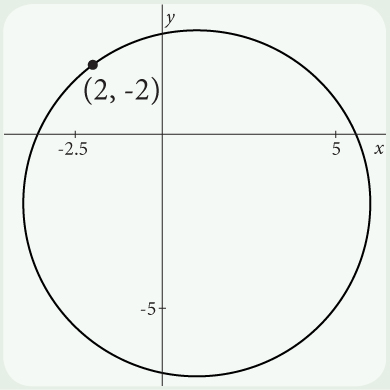
\includegraphics[height=3cm]{implicit-differentiation/pictures/implicit-tangent-linea.jpg}}
\only<16->{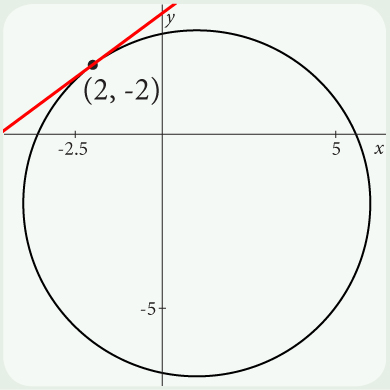
\includegraphics[height=3cm]{implicit-differentiation/pictures/implicit-tangent-lineb.jpg}}
\end{center}
\begin{align*}
\uncover<15->{&\text{Plug in} \ (-2,2):}\\
\uncover<15->{&\frac{\diff y}{\diff x}  = \frac{1+2}{4} = \frac{3}{4}}\\
\uncover<16->{&\text{Point-slope form:}\\
&y-2 = \frac{3}{4} (x+2)}
\end{align*}
\column{3in}
\abovedisplayskip=0pt
\belowdisplayskip=0pt
\abovedisplayshortskip=0pt
\belowdisplayshortskip=0pt
\begin{align*}
\uncover<2->{\text{Find} \ \frac{\diff y}{\diff x}, \ \text{given} \ (x-1)^2 \ + (y+2)^2 & = 25:} \\
\uncover<3->{\alert<handout:0|3-4>{\frac{\diff}{\diff x}\left((x-1)^2\right)} + \alert<handout:0|5-6>{\frac{\diff}{\diff x}\left((y+2)^2\right)}   &= \alert<handout:0|7-8>{\frac{\diff}{\diff x}(25)}}\\
\uncover<3->{\uncover<4->{\alert<handout:0|4>{2(x-1)\alert<handout:0|9>{\frac{\diff}{\diff x}(x-1)}}} +\uncover<6->{\alert<handout:0|6>{ 2(y+2)\alert<handout:0|11-12>{\frac{\diff}{\diff x}(y+2) }}}  &= \uncover<8->{\alert<handout:0|8>{0}}}\\
\uncover<9->{2(x-1)\alert<handout:0|9-10> {(\uncover<10->{1})}+ 2(y+2)\alert<handout:0|11-12>{\left( \uncover<12->{\frac{\diff y}{\diff x}} \right)}  & = 0}\\
\uncover<13->{2(y+2)\left( \frac{\diff y}{\diff x} \right) & = -2(x-1)}\\
\uncover<14->{\frac{\diff y}{\diff x} &=  \frac{1-x}{y+2}}
\end{align*}
\end{columns}
\end{example}
\end{frame}
% end module implicit-tangent-line
% begin module implicit-differentiation-ex3
\begin{frame}
\begin{example}[Example 3, p. 168]
\abovedisplayskip=0pt
\belowdisplayskip=-15pt
\abovedisplayshortskip=0pt
\belowdisplayshortskip=0pt
\begin{align*}
\text{Find $y'$ if }\sin (x+y) & = y^2\cos x.\\
\uncover<2->{%
\alert<handout:0| 3-4>{\frac{\diff}{\diff x} (\sin (x+y))}%
}%
& \uncover<2->{ = } %
\uncover<2->{%
\alert<handout:0| 5-6>{\frac{\diff}{\diff x} (y^2\cos x)}%
}\\%
\uncover<4->{%
\alert<handout:0| 3-4>{(\cos(x+y))\alert<handout:0| 7-8>{\frac{\diff}{\diff x}(x+y)}}%
}%
& \uncover<3->{ = } %
\uncover<6->{%
\alert<handout:0| 5-6>{(y^2)\alert<handout:0| 9-10>{\frac{\diff}{\diff x}(\cos x)} + (\cos x) \alert<handout:0| 11-12>{\frac{\diff}{\diff x}(y^2)}}%
}\\%
\uncover<7->{%
(\cos(x+y))\alert<handout:0| 7-8>{\left(\uncover<8->{1+y'}\right)}%
}%
& \uncover<7->{ = } %
\uncover<7->{%
(y^2)\alert<handout:0| 9-10>{(\uncover<10->{-\sin x})} + (\cos x) \alert<handout:0| 11-12>{(\uncover<12->{2yy'})}%
}\\%
\uncover<13->{%
\cos(x+y) + y'\cos(x+y)%
}%
& \uncover<13->{ = %
-y^2\sin x +2yy'\cos x%
}\\%
\uncover<14->{%
\alert<handout:0| 15>{y'}\cos(x+y) - 2y\alert<handout:0| 15>{y'}\cos x%
}%
& \uncover<14->{ = %
-y^2\sin x -\cos(x+y)%
}\\%
\uncover<15->{%
\text{Factor:}\quad%
\alert<handout:0| 15>{y'}(\cos(x+y) - 2y\cos x)%
}%
& \uncover<15->{ = %
-y^2\sin x -\cos(x+y)%
}\\%
\uncover<16->{%
y'%
}%
& \uncover<16->{ = } %
\uncover<16->{%
\frac{-y^2\sin x - \cos(x+y)}{\cos (x+y) - 2y\cos x}.%
}%
\end{align*}
\end{example}
\end{frame}
% end module implicit-differentiation-ex3

% begin module implicit-trig
\begin{frame}
\begin{example}[Implicit Differentiation]
\abovedisplayskip=0pt
\belowdisplayskip=-15pt
\abovedisplayshortskip=0pt
\belowdisplayshortskip=0pt
\begin{align*}
\text{Find $y'$ if } \tan xy &= x^2-y^2.\\
\uncover<2->{\alert<handout:0|3-4>{\frac{\diff}{\diff x}(\tan xy)}&= \alert<handout:0|5-6>{ \frac{\diff}{\diff x}(x^2-y^2)}}\\
\uncover<3->{\alert<handout:0|4>{\uncover<4->{(\sec^2xy)\alert<handout:0|7-8>{\frac{\diff}{\diff x}(xy)}}} & = \uncover<6->{\alert<handout:0|6>{ 2x-2yy'}}}\\
\uncover<7->{\alert<handout:0|7-8>{\left(\uncover<8->{y\alert<handout:0|9-10>{\frac{\diff}{\diff x}(x)}+x\alert<handout:0|11-12>{\frac{\diff}{\diff x}(y)}}\right)}\sec^2 xy &= 2x -2yy'}\\
\uncover<9->{\left(y\alert<handout:0|9-10>{(\uncover<10->{1})}+x\alert<handout:0|11-12>{(\uncover<12->{y'})}\right)\sec^2 xy &= 2x -2yy'}\\
\uncover<13->{y\sec^2xy+xy' \sec^2xy &= 2x -2yy'}\\
\uncover<14->{xy' \sec^2xy+2yy'&=2x-y\sec^2xy}\\
\uncover<15->{y'(x\sec^2xy+2y) &= 2x-y\sec^2xy}\\
\uncover<16->{y'&=\frac{2x-y\sec^2xy}{x\sec^2xy+2y}.}
\end{align*}
\end{example}
\end{frame}
% end module implicit-trig

% begin module implicit-differentiation-ex4
\begin{frame}
\begin{example}
%\uncover<2->{Differentiate implicitly:}%
\abovedisplayskip=0pt
\belowdisplayskip=0pt
\abovedisplayshortskip=0pt
\belowdisplayshortskip=0pt
\begin{align*}
\text{Find $y''$ if } \alert<handout:0| 14>{x^4 + y^4} & \alert<handout:0| 14>{ = 16}. \\
\uncover<2->{%
4x^3 + 4y^3y'%
}%
& \uncover<2->{ = } %
\uncover<2->{%
0%
}\\%
\uncover<3->{%
\alert<handout:0| 10>{y'}%
}%
& \uncover<3->{ \alert<handout:0| 10>{=} } %
\uncover<3->{%
\alert<handout:0| 10>{-\frac{x^3}{y^3}}.%
}\\%
\uncover<4->{%
y''%
}%
& \uncover<4->{ = } %
\uncover<4->{%
\frac{\diff}{\diff x}\left( -\frac{x^3}{y^3}\right)%
}  \uncover<5->{ = } %
\uncover<5->{%
- \frac{y^3 \alert<handout:0| 6-7>{\frac{\diff}{\diff x}(x^3)} - x^3\alert<handout:0| 8-9>{\frac{\diff}{\diff x}(y^3)}}{(y^3)^2}%
}\\%
& \uncover<6->{ = } %
\uncover<6->{%
- \frac{y^3 (\alert<handout:0| 6-7>{\uncover<7->{3x^2}}) - x^3(\alert<handout:0| 8-9>{\uncover<9->{3y^2\alert<handout:0| 10>{y'}}})}{y^6}%
} \uncover<10->{ = }%
\uncover<10->{%
- \frac{3x^2y^3  - 3x^3y^2\alert<handout:0| 10>{\left( -\frac{x^3}{y^3}\right)}}{y^6}%
}\\%
& \uncover<11->{ = } %
\uncover<11->{%
- \frac{3x^2(y^3+\frac{x^4}{y})}{y^6}%
} \uncover<12->{ = }%
\uncover<12->{%
- \frac{3x^2\left( \frac{y^4+x^4}{\alert<handout:0| 13>{y}}\right)}{\alert<handout:0| 13>{y^6}}%
}\\%
& \uncover<13->{ = } %
\uncover<13->{%
- \frac{3x^2(\alert<handout:0| 14>{y^4+x^4})}{\alert<handout:0| 13>{y^7}}%
}  \uncover<14->{ = }%
\uncover<14->{%
- \frac{3x^2(\alert<handout:0| 14>{16})}{y^7}%
} \uncover<15->{ = }%
\uncover<15->{%
-48 \frac{x^2}{y^7}.%
}%
\end{align*}
\end{example}
\end{frame}
% end module implicit-differentiation-ex4

%\input{../../modules/implicit-differentiation/implicit-second-derivative}
% end lecture

% begin lecture
\lect{February 14, 2014}{Lecture  6}{6}
\section{Exponential Functions}
% begin module exponential-function-def
\begin{frame}
\frametitle{(1.5) Exponential Functions}
The function $f(x) = 2^x$ is called an exponential function because the variable $x$ is the exponent.
\begin{columns}[c]
\column{.5\textwidth}
\only<handout:0| -2>{%
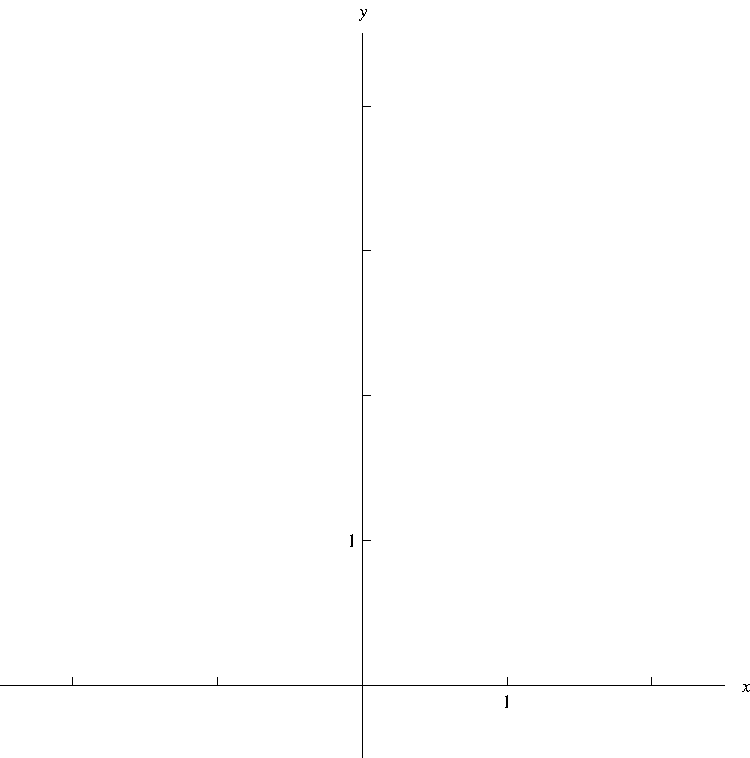
\includegraphics[height=6cm]{exponential-functions/pictures/twoxa.pdf}%
}%
\only<handout:0| 3-4>{%
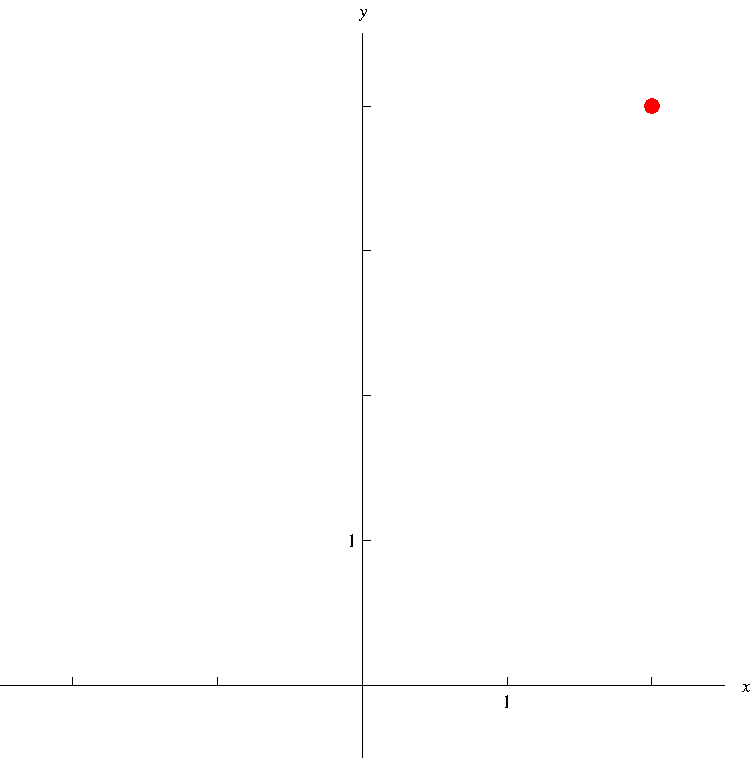
\includegraphics[height=6cm]{exponential-functions/pictures/twoxb.pdf}%
}%
\only<handout:0| 5-6>{%
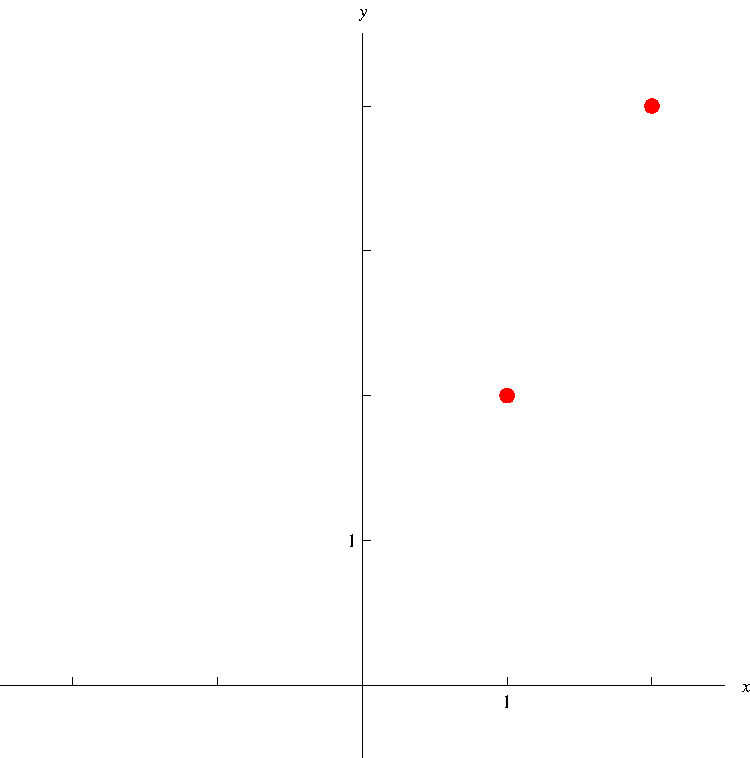
\includegraphics[height=6cm]{exponential-functions/pictures/twoxc.pdf}%
}%
\only<handout:0| 7-8>{%
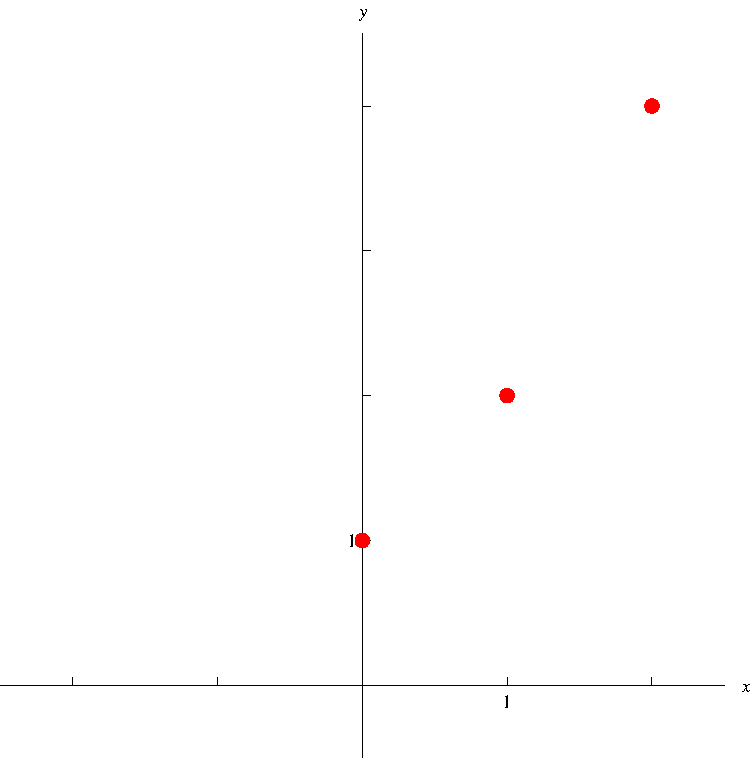
\includegraphics[height=6cm]{exponential-functions/pictures/twoxd.pdf}%
}%
\only<handout:0| 9-10>{%
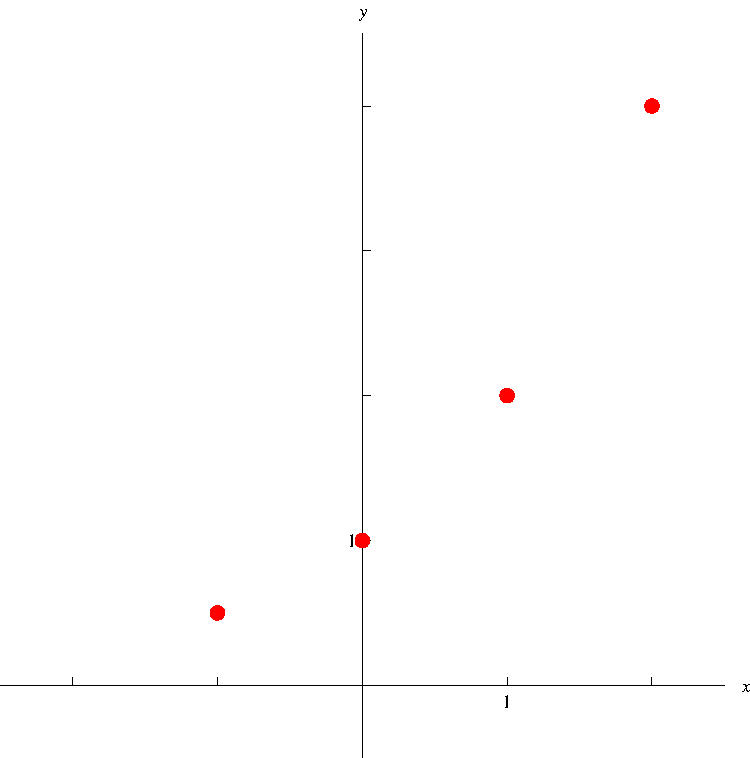
\includegraphics[height=6cm]{exponential-functions/pictures/twoxe.pdf}%
}%
\only<handout:0| 11>{%
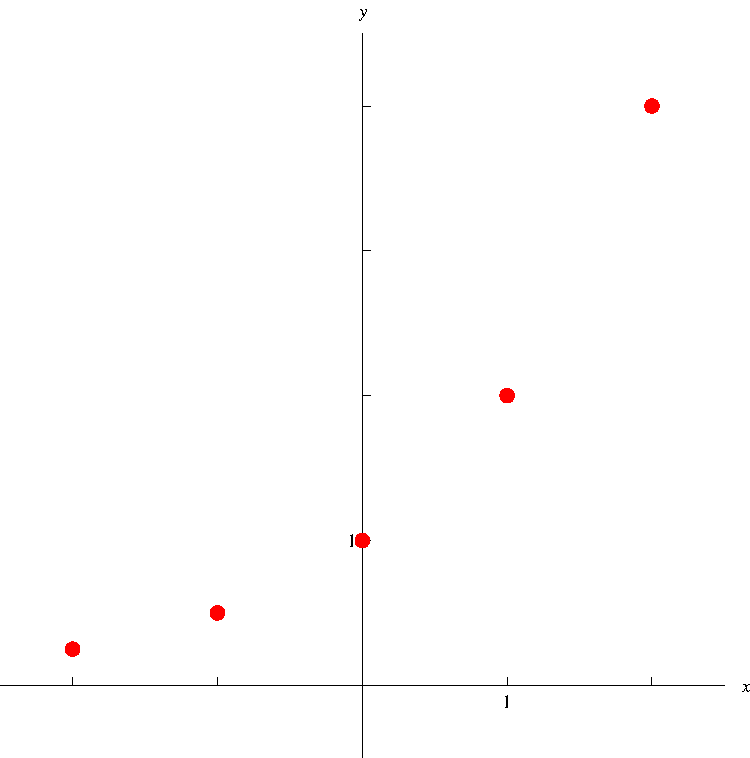
\includegraphics[height=6cm]{exponential-functions/pictures/twoxf.pdf}%
}%
\only<handout:1| 12->{%
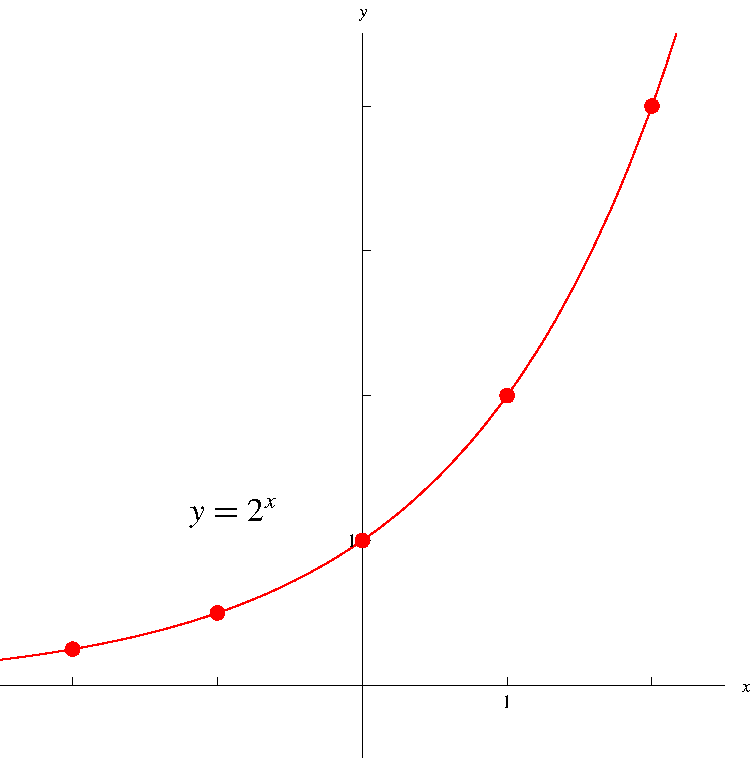
\includegraphics[height=6cm]{exponential-functions/pictures/twoxg.pdf}%
}%
\column{.5\textwidth}
\[
\begin{array}{r|l}
x & y\\
\hline
\alert<handout:0| 2-3>{2} & \alert<handout:0| 3>{\uncover<3->{4}} \\
\alert<handout:0| 4-5>{1} & \alert<handout:0| 5>{\uncover<5->{2}} \\
\alert<handout:0| 6-7>{0} & \alert<handout:0| 7>{\uncover<7->{1}} \\
\alert<handout:0| 8-9>{-1} & \alert<handout:0| 9>{\uncover<9->{1/2}} \\
\alert<handout:0| 10-11>{-2} & \alert<handout:0| 11>{\uncover<11->{1/4}} 
\end{array}
\]
\uncover<13->{
\begin{definition}[Exponential Function]
In general, an exponential function is a function of the form $f(x) = a^x$, where $a$ is a positive constant.
\end{definition}
}
\end{columns}
\end{frame}
% end module exponential-function-def

% begin module exponential-def-various-approaches
\begin{frame}
\frametitle{Exponents overview}
\begin{itemize}
\item<1-> Previously, for fixed $x$, we studied $a^{x}$ as a function of $a$. 
\item<2-> In present lecture we study $f(x)=a^x$ as a function of $x$.
\item<3-> A construction of $a^x$ was previously promised.
\item<4-> There are several equivalent ways of defining $a^x$. 
\item<5-> We give the easiest definition. 
\item<6-> We give a second equivalent definition. The second definition is studied in detail in Calculus II. 
\item<7->We discuss pros and cons.
\end{itemize}
\end{frame}
\begin{frame}
\frametitle{Exponent definition using limits (approach I)}
\begin{itemize}
\item<1-> For integer $p$ we know to compute $a^p$.
\item<2-> Therefore for integer $q$ we know to compute $a^{\frac{1}{q}}= \sqrt[q]{a}=\max\{x|\text{~for~which~} x^q\leq a\}$.
\item<3-> Therefore we know to compute $a^{\frac{p}{q}}$ for all rational $\frac{p}{q}$.
\item<4-> We can then define
\[
a^x = \lim\limits_{\substack{y \to x \\ y\text{-rational}}} a^y 
\]
\item<5-> Not computationally effective. It is not how computers compute.
\item<6-> However is the easiest approach. $a^{x+y}=a^xa^y$ is easiest to prove (follows directly from the $\varepsilon, \delta$-definition of $\lim$).
\item<7->\alert<7->{This is the definition assumed in Calculus I.}
\end{itemize}
\end{frame}
\begin{frame}
\frametitle{Exponent definition using series (approach II)}
\begin{itemize}
\item<1-> The Calc II formula can be used as alternative definition.
\[
e^{x}=\alert<4>{\sum_{n=0}^{\infty}} \frac{x^n}{\alert<2>{n!}}= 1+ x+\frac{x^2}{2!}+\frac{x^3}{3!}+\dots + \frac{x^{n}}{\alert<2>{n!}}+\dots
\]
\uncover<2->{\alert<2>{Here $n!=1\cdot 2\cdot 3\cdot\dots \cdot(n-1)\cdot n$ and is read ``$n$ factorial''. }}
\item<3-> For $|x|<1$ define 
\[
\ln (1+x)=\alert<4>{\sum_{n=1}^{\infty}} (-1)^{n+1}\frac{x^n}{n}=  x-\frac{x^2}{2}+\frac{x^3}{3}-\dots + \frac{(-1)^{n+1}x^{n}}{n}+\dots
\]
\uncover<4->{\alert<4>{Infinite sum studied in Calc II.}} 
\item<5-> For arbitrary $a>0$ define $a^x$ as $a^x=e^{x\ln a}$. 
\item<6-> Disadvantage: more difficult to prove $e^{x+y}=e^{x}e^y$ and $e^{\ln(1+x)}=1+x$, proof done in Calculus II.
\item<7-> This is how computers compute $e^x$ and $a^x$.
\end{itemize}
\end{frame}

% end module exponential-def-various-approaches

% begin module exponential-function-graphs
\begin{frame}
\begin{center}
Graphs of various exponential functions.

\psset{xunit=2cm, yunit=2cm}
\begin{pspicture}(-5, -5)(5,5) 
\psframe*[linecolor=white](-5,-5)(5,5) 
\psaxes[labels=none]{<->}(0,0)(-2.1,-0.2)(2.1,3.5)
\uncover<1->{
\rput[r](1.8, 2.3){$y=2^x$}
%Function formula: 2^{x} 
\psplot[linecolor=red, plotpoints=1000]{-2}{1.584962501}{2 x exp }
}
\uncover<2->{
\rput[l](1.2, 3.1){$y=4^x$}
%Function formula: 4^{x} 
\psplot[linecolor=black, plotpoints=1000]{-2}{0.79248125}{4 x exp }
}
\uncover<3->{
\rput[b](0.4, 3.05){$y=10^x$}
%Function formula: 4^{x} 
\psplot[linecolor=blue, plotpoints=1000]{-2}{0.477121255}{10 x exp }
}
\uncover<4->{
\rput[l](1.15, 1.5){$y=1.5^x$}
%Function formula: 4^{x} 
\psplot[linecolor=green, plotpoints=1000]{-2}{2}{1.5 x exp }
}
\uncover<5->{
\rput[l](-1.9, 2){$y=0.5^x$}
%Function formula: 4^{x} 
\psplot[linecolor=purple, plotpoints=1000]{-1.584962501}{2}{0.5 x exp }
}
\uncover<6->{
\rput[l](-1.2, 3.1){$y=0.25^x$}
%Function formula: 4^{x} 
\psplot[linecolor=brown, plotpoints=1000]{-0.79248125}{2}{0.25 x exp }
}
\end{pspicture}
\pause\pause\pause\pause\pause
%\ \only<handout:0| -1>{%
%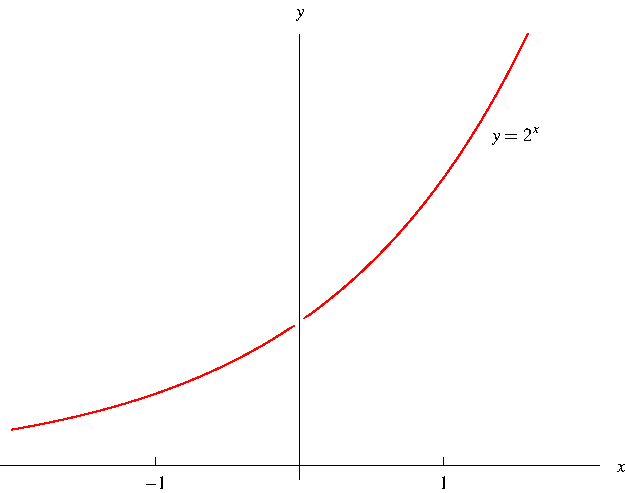
\includegraphics[height=6cm]{exponential-functions/pictures/07-02-manyexpa.pdf}%
%}%
%\only<handout:0| 2>{%
%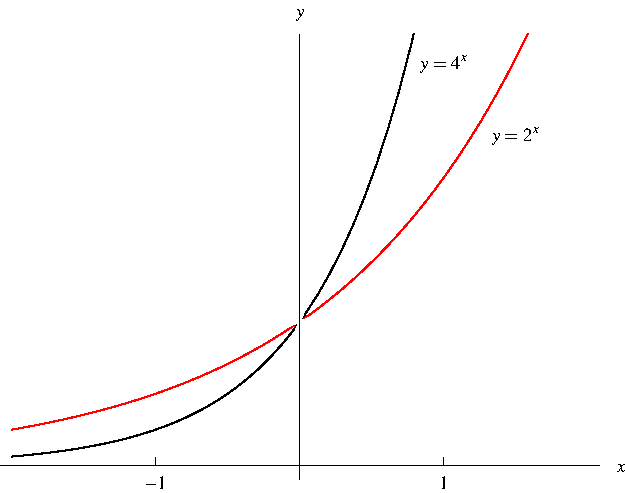
\includegraphics[height=6cm]{exponential-functions/pictures/07-02-manyexpb.pdf}%
%}%
%\only<handout:0| 3>{%
%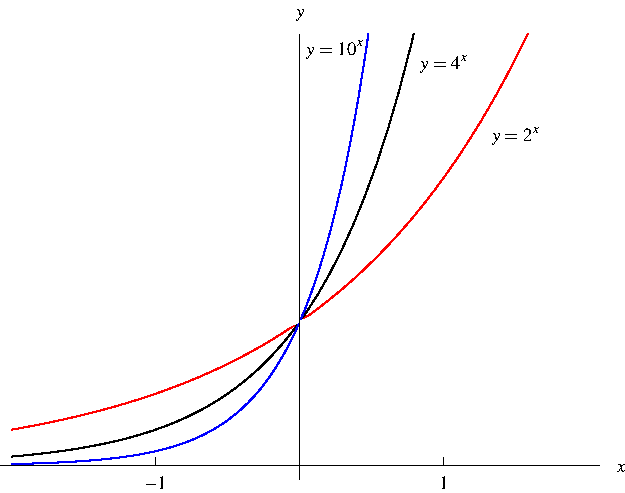
\includegraphics[height=6cm]{exponential-functions/pictures/07-02-manyexpc.pdf}%
%}%
%\only<handout:0| 4>{%
%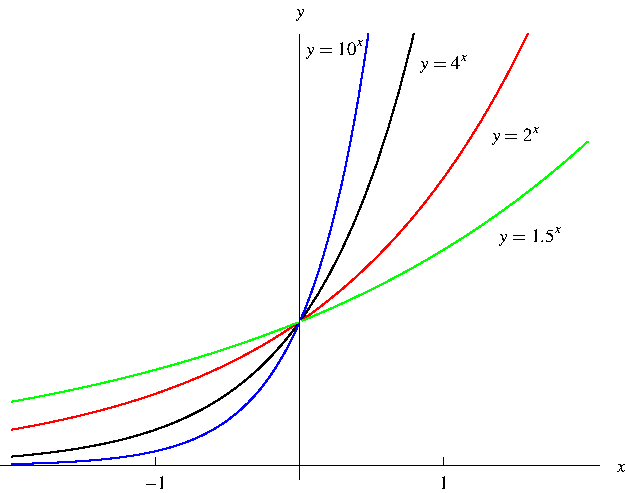
\includegraphics[height=6cm]{exponential-functions/pictures/07-02-manyexpd.pdf}%
%}%
%\only<handout:0| 5>{%
%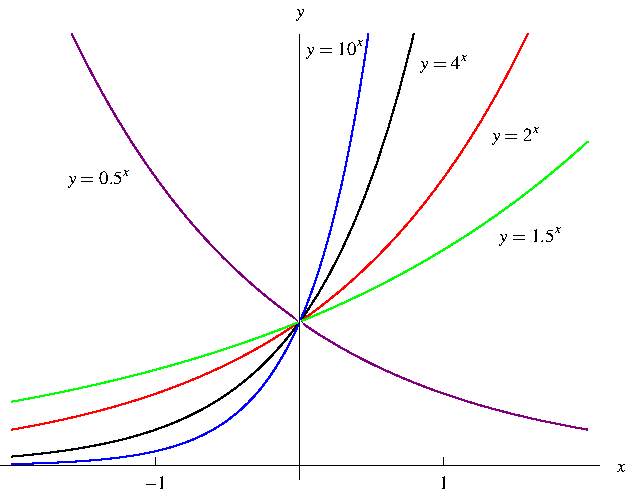
\includegraphics[height=6cm]{exponential-functions/pictures/07-02-manyexpe.pdf}%
%}%
%\only<6->{%
%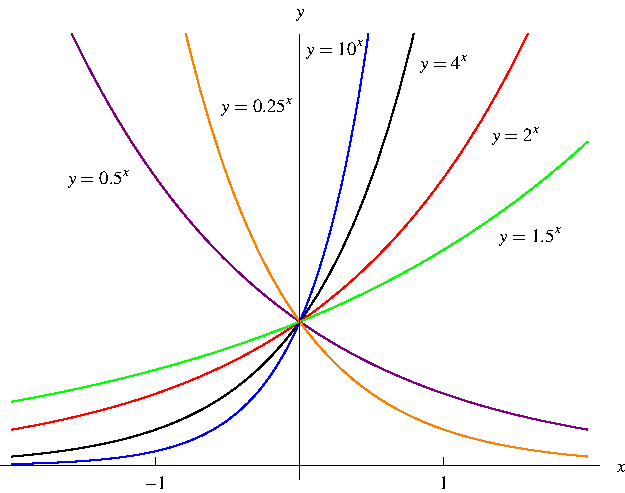
\includegraphics[height=6cm]{exponential-functions/pictures/07-02-manyexpf.pdf}%
%}%

\end{center}
\end{frame}
% end module exponential-function-graphs

% begin module exponential-versus-polynomial
\begin{frame}
\begin{center}
\small
Graphical comparison of $y = 2^x$ with $y = x^2$. Axes have different scales.
\begin{tabular}{cc}
\uncover<1->{
\psset{xunit=0.8cm, yunit=0.1cm}
\begin{pspicture}(-5, -5)(5,5) 
\psframe*[linecolor=white](-5,-5)(5,5) 
\psaxes[ticks=x, labels=x]{<->}(0,0)(-1,-3)(5.01,60)
\psline(-0.1,40)(0.1, 40)
\rput[l](0.2, 40){$40$} 
\psline(-0.1,20)(0.1, 20)
\rput[l](0.2, 20){$20$} 
%Function formula: 2^{x} 
\psplot[linecolor=red, plotpoints=1000]{-0.5}{5}{2 x exp }
\psplot[linecolor=blue, plotpoints=1000]{-0.5}{5}{x 2 exp }
\end{pspicture}
%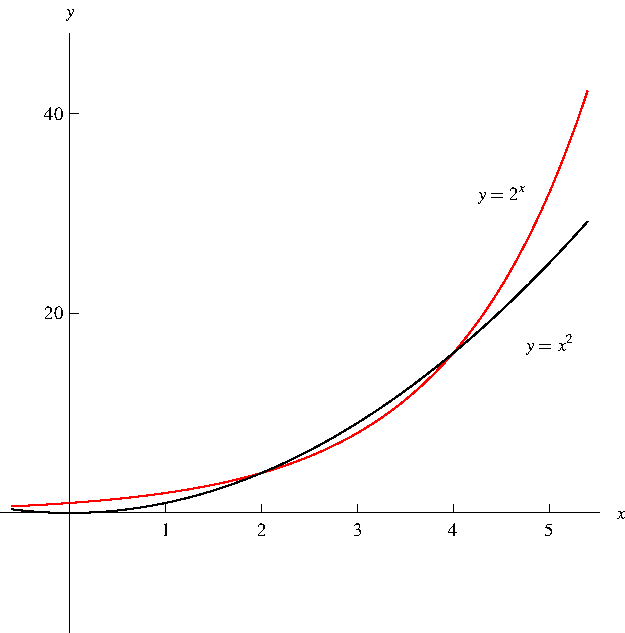
\includegraphics[height=5cm]{exponential-functions/pictures/07-02-expvspowera.pdf}%
}
&%
\uncover<2->{
\psset{xunit=0.25cm, yunit=0.05cm}
\begin{pspicture}(-5, -5)(5,5) 
\psframe*[linecolor=white](-5,-5)(5,5) 
\psaxes[ticks=x, Dx=4, labels=x]{<->}(0,0)(-1,-8)(16,120)
\psline(-0.4,100)(0.4, 100)
\rput[l](0.6, 100){$100$} 
%Function formula: 2^{x} 
\psplot[linecolor=red, plotpoints=1000]{-0.5}{7}{2 x exp }
\psplot[linecolor=blue, plotpoints=1000]{-0.5}{11.313708499}{x 2 exp }
\psline(-0.5, -3.5)(5, -3.5)(5, 32)(-0.5, 32)(-0.5, -3.5)
\rput[l](6, 10){Magnified region}
\end{pspicture}
%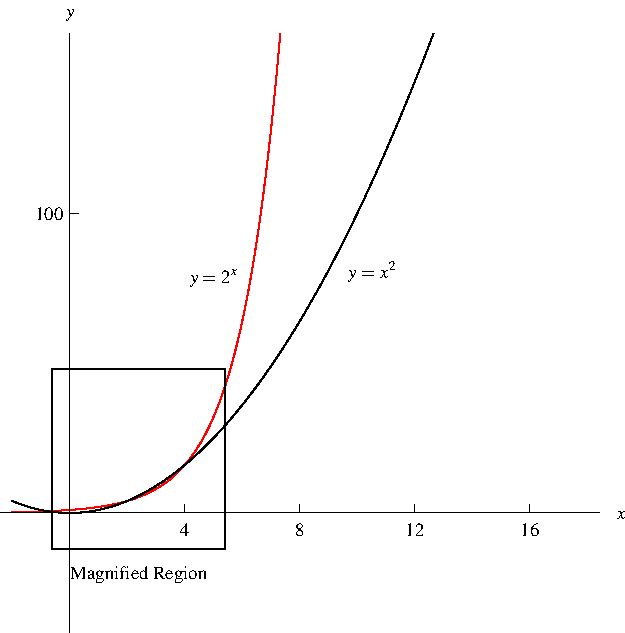
\includegraphics[height=5cm]{exponential-functions/pictures/07-02-expvspowerb.pdf}%
}
\end{tabular}
\end{center}
\end{frame}
% end module exponential-versus-polynomial
% begin module exponential-function-ex-sketch
\begin{frame}
\begin{example}
Draw the graph of the function $y = 2^{-x}-1$.
\only<handout:0| -1>{%
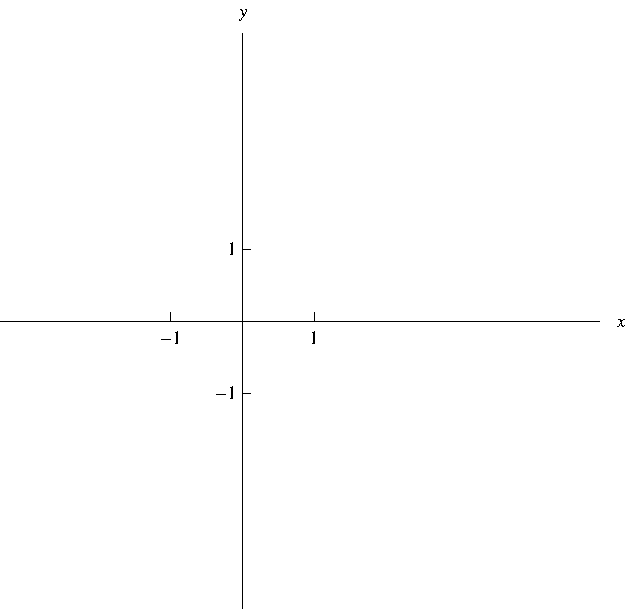
\includegraphics[height=7cm]{exponential-functions/pictures/07-02-ex1a.pdf}%
}%
\only<handout:0| 2>{%
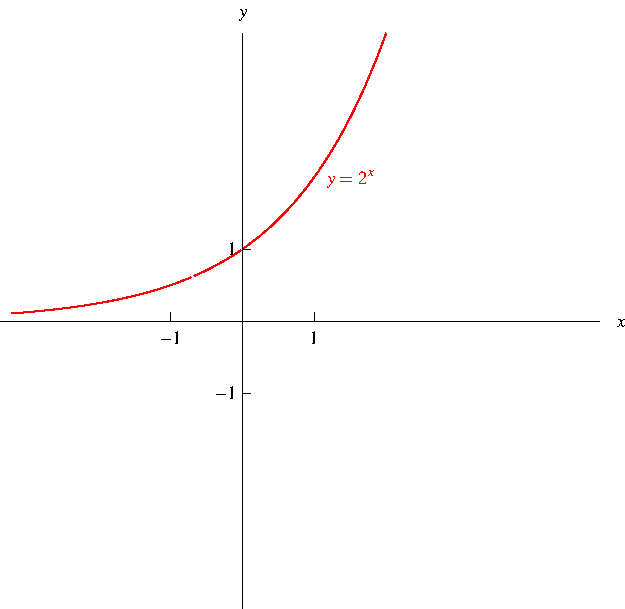
\includegraphics[height=7cm]{exponential-functions/pictures/07-02-ex1b.pdf}%
}%
\only<handout:0| 3>{%
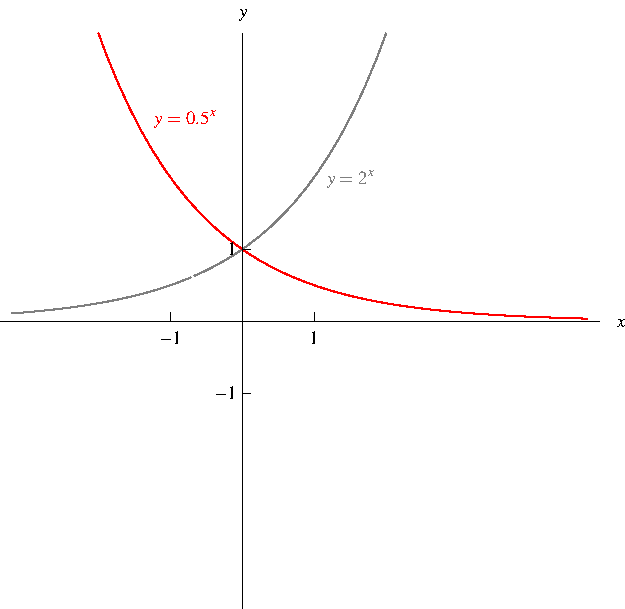
\includegraphics[height=7cm]{exponential-functions/pictures/07-02-ex1c.pdf}%
}%
\only<4->{%
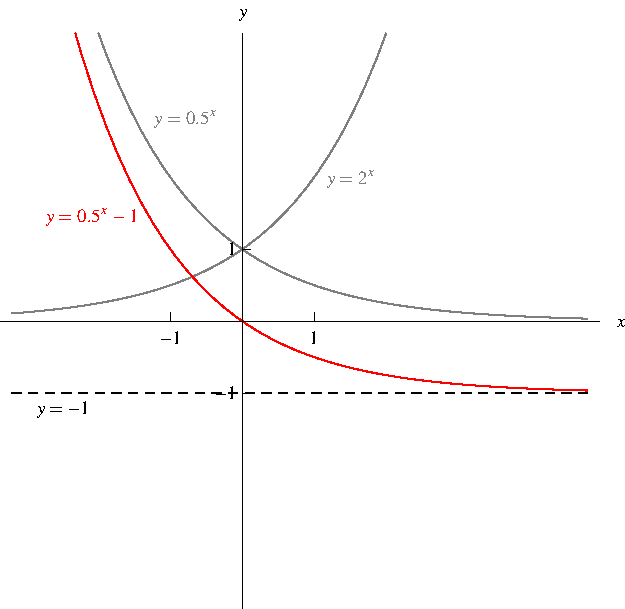
\includegraphics[height=7cm]{exponential-functions/pictures/07-02-ex1d.pdf}%
}%
\end{example}
\end{frame}
% end module exponential-function-ex-sketch

\subsection{The Natural Exponential Function}
% begin module natural-exponential-intro
\begin{frame}
\frametitle{The Natural Exponential Function}
\begin{itemize}
\item  One base for an exponential function is especially useful.
\item<2->  It has a special property: its tangent line at $x = 0$ has slope $m=1$.
\item<3->  We call this number $e$, known as Euler's number or Napier's constant.
\item<4->  $e$ is a number between 2 and 3.  
\item<5-> In fact, $e = 1+1+\frac{1}{2!}+\frac{1}{3!} +\frac{1}{4!}+\dots\approx 2.71828$.  
\end{itemize}

\begin{columns}
\column{.3\textwidth}
\psset{xunit=1.3cm, yunit=1.3cm}
\begin{pspicture}(-1.4, -0.5)(1.4,2.6)
\psaxes[labels=none]{<->}(0,0)(-1.3, -0.5)(1.3,2.5)
\psplot[linecolor=red, plotpoints=1000]{-1.3}{1.3}{2 x exp}
\rput[r](-0.2, 1.1){\footnotesize $y=2^x$}
\rput[l](0.2, 0.8){\tiny $m\approx 0.693147$} 
\psline[linecolor=blue](-1.3,0.098908665)(1.3, 1.901091335)
\end{pspicture}
%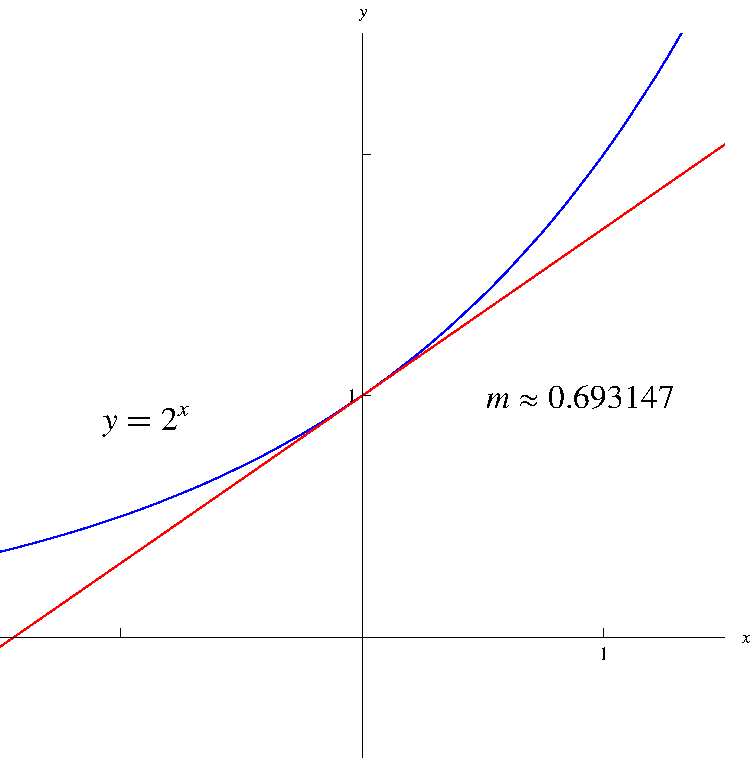
\includegraphics[height=4cm]{exponential-functions/pictures/exp-tangent-two.pdf}%
\column{.3\textwidth}
\uncover<handout: 1|3->{%
\psset{xunit=1.3cm, yunit=1.3cm}
\begin{pspicture}(-1.4, -0.5)(1.4,2.6)
\psaxes[labels=none]{<->}(0,0)(-1.3, -0.5)(1.3,2.5)
\psplot[linecolor=red, plotpoints=1000]{-1.3}{0.901091335}{2.718281828 x exp}
\rput[r](-0.2, 1.1){\footnotesize $y=e^x$}
\rput[l](0.2, 0.8){\tiny $m=1$}
\psline[linecolor=blue](-1.3, -0.3)(1.3,2.3) 
\end{pspicture}
%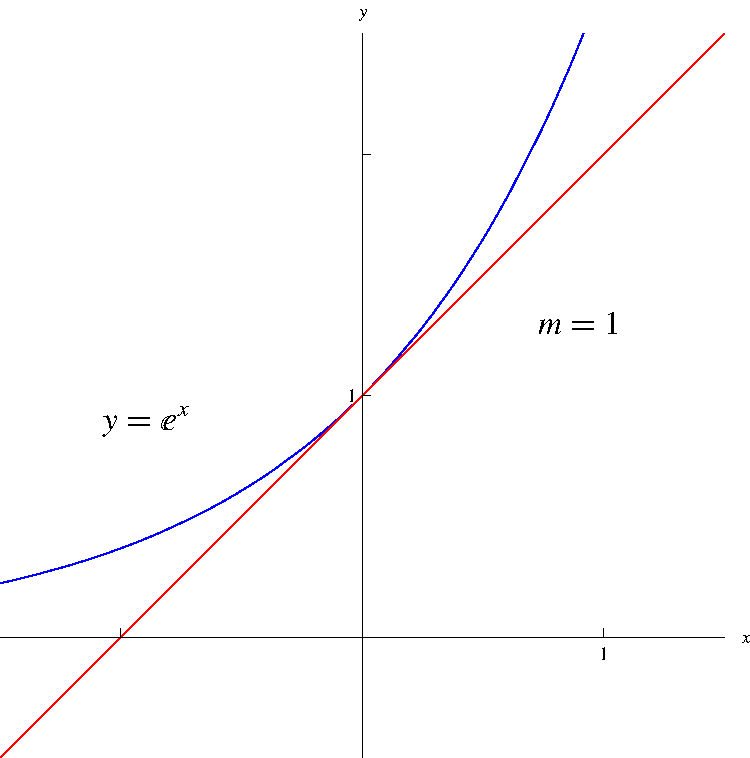
\includegraphics[height=4cm]{exponential-functions/pictures/exp-tangent-e.pdf}%
}%
\column{.3\textwidth}
\psset{xunit=1.3cm, yunit=1.3cm}
\begin{pspicture}(-1.4, -0.5)(1.4,2.6)
\psaxes[labels=none]{<->}(0,0)(-1.3, -0.5)(1.3,2.5)
\psplot[linecolor=red, plotpoints=1000]{-1.3}{0.82020868}{3 x exp}
\rput[r](-0.2, 1.1){\footnotesize $y=3^x$}
\rput[l](0.2, 0.8){\tiny $m\approx 1.09861$} 
\psline[linecolor=blue](-1.3, -0.428195975)(1.3,2.428195975)
\end{pspicture}
%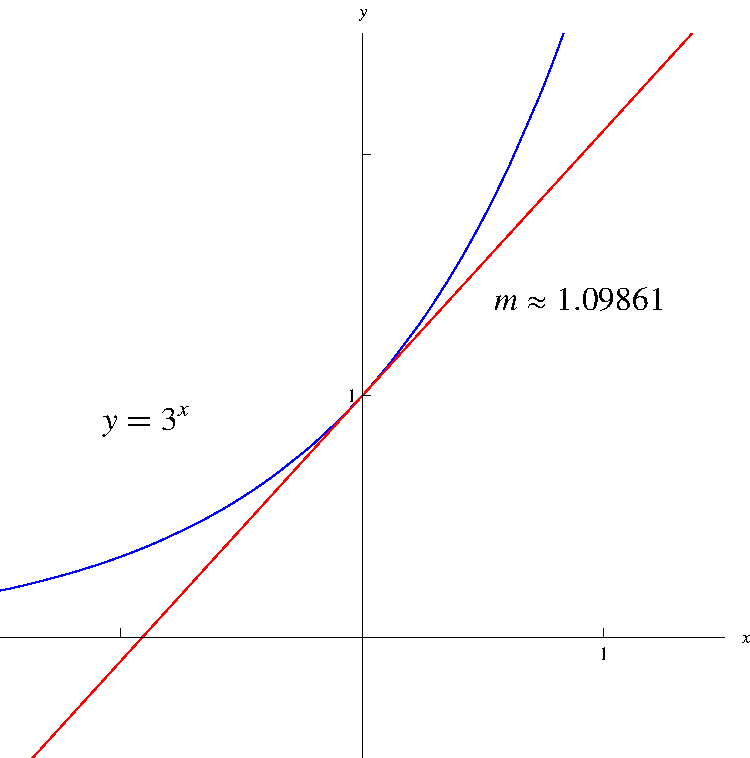
\includegraphics[height=4cm]{exponential-functions/pictures/exp-tangent-three.pdf}%
\end{columns}
\end{frame}
% end module natural-exponential-intro
\section{Differentiation Formulas}
\subsection{Derivatives of Exponential Functions}
% begin module exponential-function-derivative
\begin{frame}
\frametitle{Derivatives of Exponential Functions}
Compute the derivative of $f(x) = a^x$ using the definition:
\begin{eqnarray*}
\uncover<2->{f'(x) = \lim_{h\rightarrow 0} \frac{f(x+h)-f(x)}{h}} & \uncover<3->{=} & \uncover<3->{\lim_{h\rightarrow 0} \frac{a^{x+h}-a^x}{h}}\\
 & \uncover<4->{=} & \uncover<4->{\lim_{h\rightarrow 0} \frac{a^x a^h-a^x}{h}}\\
 & \uncover<5->{=} & \uncover<5->{\lim_{h\rightarrow 0} \frac{a^x (a^h- 1)}{h}}\\
 & \uncover<6->{=} & \uncover<6->{a^x \lim_{h\rightarrow 0} \frac{a^h- 1}{h}}\\
\end{eqnarray*}
\uncover<7->{%
Note that the limit is the value of the derivative at 0; that is,
\[
f'(0) = \lim_{h\rightarrow 0}\frac{a^h-1}{h} .
\]
}%
\end{frame}


\begin{frame}
We have shown that, if $f(x) = a^x$ is differentiable at 0, then it is differentiable everywhere, and
\[
f'(x) = f'(0)a^x .
\]
\uncover<2->{
It is a fact that, for all positive $a$, the limit $\lim_{h\rightarrow 0}\frac{a^h - 1}{h}$ exists (we will not prove this).  Approximations for $a = 2$ and $a = 3$ appear below.
\[
\lim_{h\rightarrow 0}\frac{2^h - 1}{h} \approx 0.693147, \qquad %
\lim_{h\rightarrow 0}\frac{3^h - 1}{h} \approx 1.098612.
\]
}
\uncover<3->{
Then the derivative of $f(x) = a^x$ exists for all positive $a$.  Approximations for $a = 2$ and $a = 3$ appear below.
\[
\frac{\diff }{\diff x}(2^x) \approx (0.69)2^x, \qquad %
\frac{\diff }{\diff x}(3^x) \approx (1.10)3^x.
\]
}
\end{frame}
% end module exponential-function-derivative

% begin module e-def
\begin{frame}
\[
\text{If}\quad  f(x) = a^x, \quad \text{then}\quad f'(x) = f'(0)a^x .
\]
The formula above is simplest when $f'(0) = 1$.  Since $\lim\limits_{h\rightarrow 0}\frac{2^h-1}{h}\approx 0.69$ and $\lim\limits_{h\rightarrow 0}\frac{3^h-1}{h}\approx 1.10$, we expect there is a number $a$ between 2 and 3 such that $\lim\limits_{h\rightarrow 0}\frac{a^h-1}{h} = 1$.  
\uncover<2->{
\begin{definition}[$e$]
$e$ is the number such that $\lim\limits_{h\rightarrow 0}\frac{e^h-1}{h} = 1$.
\end{definition}
}

\begin{columns}
\column{.3\textwidth}
\psset{xunit=1.1cm, yunit=1.1cm}
\begin{pspicture}(-1.3, -0.5)(1.4,2.5) 
\psframe*[linecolor=white](-1.3,-0.5)(1.5,2.5) 
\psaxes[labels=none]{<->}(0,0)(-1.3, -0.5)(1.3,2.5)
\psplot[linecolor=red, plotpoints=1000]{-1.3}{1.3}{2 x exp}
\rput[r](-0.2, 1.1){\footnotesize $y=2^x$}
\rput[l](0.2, 0.8){\tiny $m\approx 0.693147$} 
\psline[linecolor=blue](-1.3,0.098908665)(1.3, 1.901091335)
\end{pspicture}
%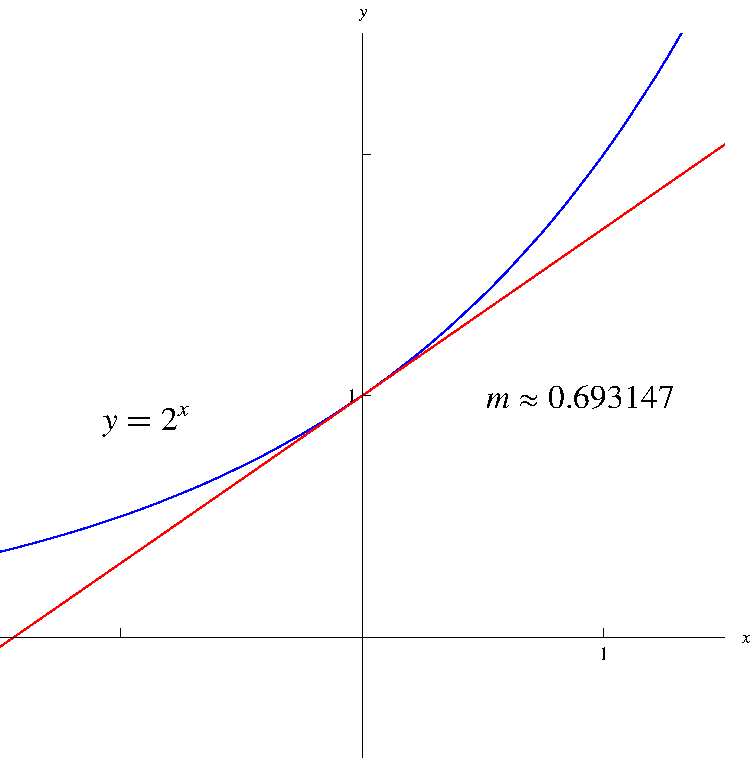
\includegraphics[height=4cm]{exponential-functions/pictures/exp-tangent-two.pdf}%
\column{.3\textwidth}
\uncover<handout: 1|3->{%
\psset{xunit=1.1cm, yunit=1.1cm}
\begin{pspicture}(-1.3, -0.5)(1.4,2.6) 
\psframe*[linecolor=white](-1.3,-0.5)(1.4,2.6) 
\psaxes[labels=none]{<->}(0,0)(-1.3, -0.5)(1.3,2.5)
\psplot[linecolor=red, plotpoints=1000] {-1.3}{0.901091335}{2.718281828 x exp}
\rput[r](-0.2, 1.1){\footnotesize $y=e^x$}
\rput[l](0.2, 0.8){\tiny $m=1$}
\psline[linecolor=blue](-1.3, -0.3)(1.3,2.3) 
\end{pspicture}
%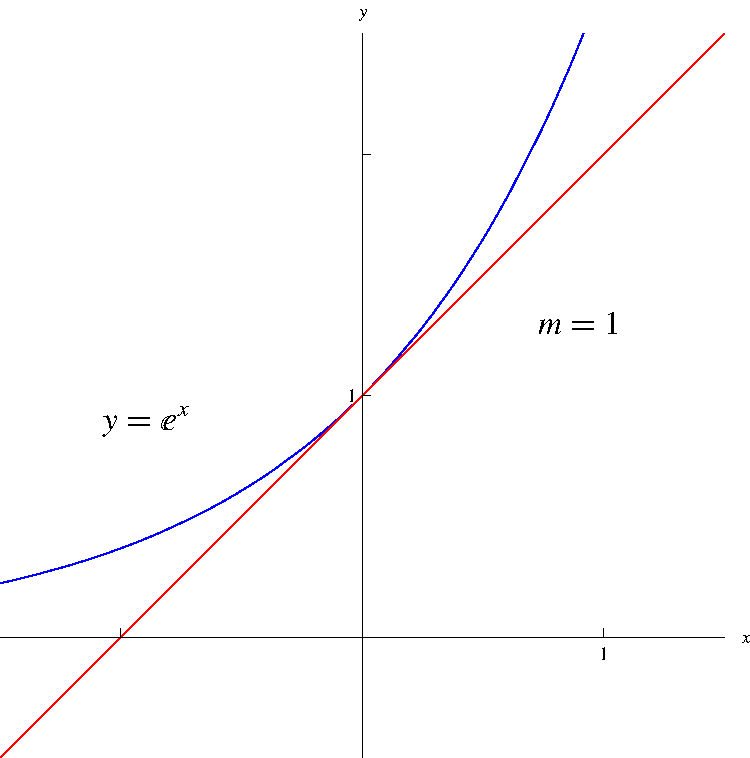
\includegraphics[height=4cm]{exponential-functions/pictures/exp-tangent-e.pdf}%
}%
\column{.3\textwidth}
\psset{xunit=1.1cm, yunit=1.1cm}
\begin{pspicture}(-1.3, -0.5)(1.4,2.6) 
\psframe*[linecolor=white](-1.3,-0.5)(1.4,2.6) 
\psaxes[labels=none]{<->}(0,0)(-1.3, -0.5)(1.3,2.5)
\psplot[linecolor=red, plotpoints=1000]{-1.3}{0.82020868}{3 x exp}
\rput[r](-0.2, 1.1){\footnotesize $y=3^x$}
\rput[l](0.2, 0.8){\tiny $m\approx 1.09861$} 
\psline[linecolor=blue](-1.3, -0.428195975)(1.3,2.428195975)
\end{pspicture}
%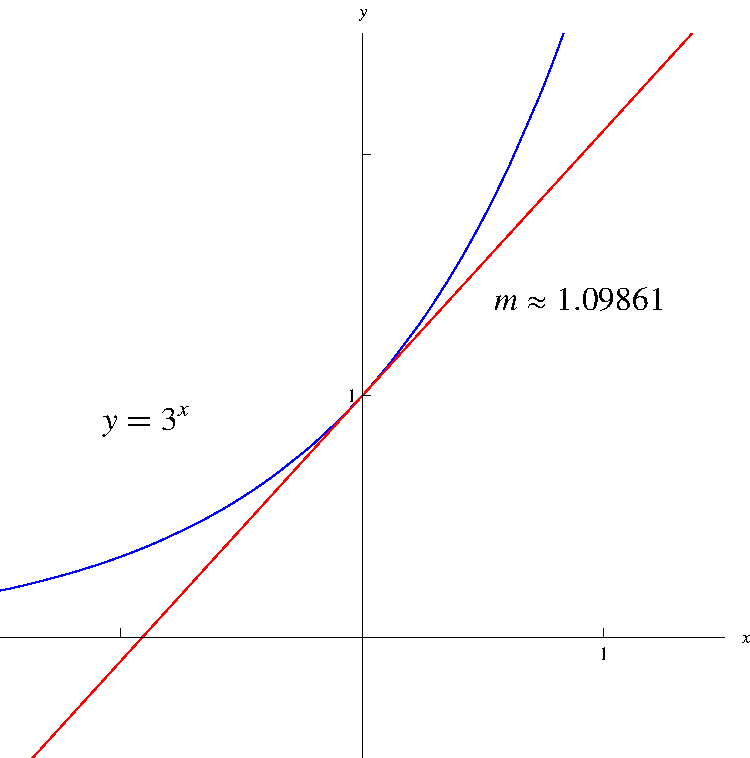
\includegraphics[height=4cm]{exponential-functions/pictures/exp-tangent-three.pdf}%
\end{columns}
\end{frame}
% end module e-def

% begin module natural-exponential-def
\begin{frame}
\begin{definition}[Natural Exponential Function]
$e^x$ is called the natural exponential function.  Its derivative is
\[
\frac{\diff}{\diff x} \left(e^x\right) = e^x .
\]
\end{definition}
\end{frame}
% end module natural-exponential-def

% begin module derivative-e-plus-polynomial
\begin{frame}
\begin{example}[Derivative of a Polynomial and the Natural Exponential Function]
\abovedisplayskip=0pt
\belowdisplayskip=-15pt
\abovedisplayshortskip=0pt
\belowdisplayshortskip=0pt
\begin{align*}
\text{Differentiate}\quad y & = e^x+x^7.\\
\uncover<2->{\frac{\diff y}{\diff x} & = \alertNoH{3-4}{\frac{\diff}{\diff x}(e^x)} + \alertNoH{5-6}{\frac{\diff}{\diff x}(x^7)}}\\
& \uncover<3->{= \fcAnswer{4}{\alertNoH{4}{e^x}}  + \fcAnswerUncover{3}{6}{\alertNoH{6}{7x^6}.}}
\end{align*}
\end{example}
\end{frame}
% end module derivative-e-plus-polynomial

% begin module chain-rule-general-exponential.tex
\begin{frame}
\begin{example}[Chain Rule, general exponential function]
\abovedisplayskip=0pt
\belowdisplayskip=0pt
\abovedisplayshortskip=0pt
\belowdisplayshortskip=0pt
\begin{align*}
\text{Differentiate}\quad y & = \alert<handout:0|2-3>{2}^x.\\
\uncover<2->{y} & \uncover<2->{= \alert<handout:0|2-3>{( e^{\uncover<3->{\ln 2}} )}^x}\\
\uncover<4->{y} & \uncover<4->{= e^{x\ln 2}.}\\
\uncover<5->{\text{Let} \quad \alert<handout:0|5-6>{\alert<handout:0|13-14>{\alert<handout:0|11-12>{u}}} &\alert<handout:0|5-6>{\alert<handout:0|11-14>{=}} \uncover<6-| handout:0>{\alert<handout:0|6>{\alert<handout:0|11-12>{\alert<handout:0|13-14>{ x\ln 2.}}}}} \\
\uncover<7->{\text{Then} \quad \alert<handout:0|9-10>{y} &\alert<handout:0|9-10>{= \uncover<7-| handout:0>{e^u.}}} \\
\uncover<8->{\text{Chain Rule:}\quad \frac{\diff y}{\diff x} &= \alert<handout:0|9-10>{ \frac{\diff y}{\diff u}}\alert<handout:0|11-12>{ \frac{\diff u}{\diff x}}}\\
\uncover<9->{&= \alert<handout:0|9-10>{(\uncover<10-| handout:0>{e^{\alert<handout:0|13-14>{u}}})}\alert<handout:0|11-12>{(\uncover<12-| handout:0>{\ln 2})} }\\
\uncover<13->{ &=} \uncover<13-| handout:0>{(e^{\alert<handout:0|13-14>{(\uncover<14->{x\ln2})}})(\ln 2)}\\
\uncover<15->{& =} \uncover<15-| handout:0>{(e^{\ln 2})^x(\ln 2)}\\
\uncover<16->{& =} \uncover<16-| handout:0>{2^x\ln 2.} 
\end{align*}
\end{example}
\end{frame}
% begin module chain-rule-general-exponential.tex

% begin module general-exponential-derivative
\begin{frame}
\begin{theorem}[The Derivative of $a^x$]
\[
\frac{\diff}{\diff x} (a^x) = a^x \ln a .
\]
\end{theorem}
\end{frame}
% end module general-exponential-derivative

% end lecture

% begin lecture
\lect{February 21, 2014}{Lecture  8}{8}
\section{Inverse Functions}
\subsection{One-to-one Functions}
% begin module one-to-one-def
\begin{frame}
\frametitle{One-to-one Functions}
\begin{definition}[One-to-one Function]
A function $f$ is a one-to-one function if it never takes on the same value twice; that is,
\[
f(x_1) \neq f(x_2) \ \text{whenever }  \ x_1 \neq x_2 .
\]
\end{definition}
\begin{columns}[c]
\column{.5\textwidth}
\psset{xunit=1.3cm, yunit=1.3cm}
\begin{pspicture}(-5, -5)(5,5) 
\psframe*[linecolor=white](-5,-5)(5,5) 
\psaxes[ticks=none, labels=none]{<->}(0,0)(-0.5,-0.5)(3.9,3)
%Function formula: -1/2*((-17/10+x)^{2})+9/5 
\psplot[linecolor=red, plotpoints=1000]{-0.5}{3.9}{1.8 x -1.7 add 2 exp -0.5 mul add }
\rput[b](1.7, 1.9) {\footnotesize $y=f(x)$}

\psFullDot{0.7}{1.3}
\rput[br](0.6, 1.4) {\footnotesize $(x_1, f(x_1))$}
\psFullDot{2.7}{1.3}
\rput[bl](2.8, 1.4) {\footnotesize $(x_2, f(x_2))$}

\psline(-0.5, 1.3)(3, 1.3)
\rput[t](1.7, 1.2) {\footnotesize $y=f(x_1)=f(x_2)$}

\psline(0.7, -0.1)(0.7, 0.1)
\rput[t](0.7, -0.2){\footnotesize $x_1$}
\psline(2.7, -0.1)(2.7, 0.1)
\rput[t](2.7, -0.2){\footnotesize $x_2$}

\end{pspicture} 
%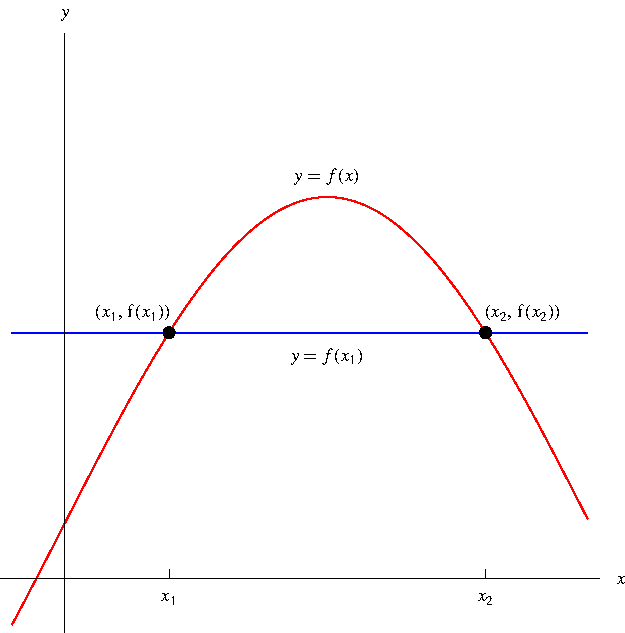
\includegraphics[height=5cm]{inverse-functions/pictures/07-01-1-1def.pdf}%
%
\column{.5\textwidth}
$\leftarrow$ This function is not one-to-one.
\end{columns}
\end{frame}
% end module one-to-one-def

% begin module horizontal-line-test
\begin{frame}
Question: How can we tell from the graph of a function whether it is one-to-one or not?

Answer: Use the horizontal line test.

\begin{proof}[The Horizontal Line Test]
A function is one-to-one if and only if no horizontal line intersects it more than once.
\end{proof}

\begin{tabular}{cc}
\psset{xunit=0.7cm, yunit=0.7cm}
\begin{pspicture}(-5, -5)(5,5) 
\psframe*[linecolor=white](-5,-5)(5,5) 
\psaxes[ticks=none, labels=none]{<->}(0,0)(-3,-3)(3,3)
%Function formula: 1/2 (x)+1/2 
\psplot[linecolor=red, plotpoints=1000]{1}{2}{0.5 x 0.5 mul add } %Function formula: (x)^{3} 
\psplot[linecolor=red, plotpoints=1000]{-1}{1}{x 3 exp } %Function formula: 3/2 (x)+1/2 
\psplot[linecolor=red, plotpoints=1000]{-2}{-1}{0.5 x 1.5 mul add }
\end{pspicture} 
%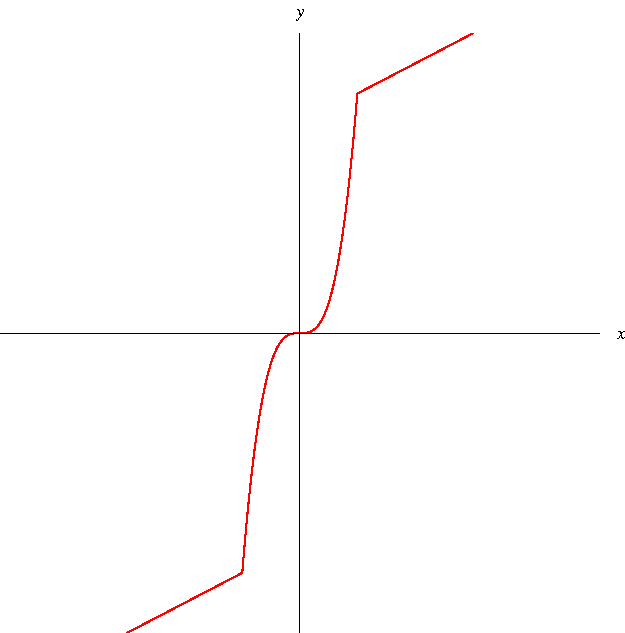
\includegraphics[height=4cm]{inverse-functions/pictures/07-01-onetoone.pdf} 
 %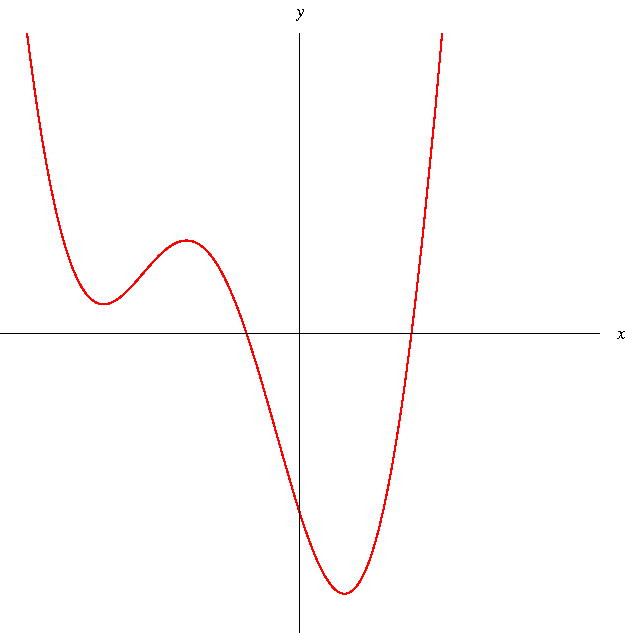
\includegraphics[height=4cm]{inverse-functions/pictures/07-01-notonetoonea.pdf}%
&%
\uncover<handout:0| 2->{%
\psset{xunit=0.7cm, yunit=0.7cm}
\begin{pspicture}(-5, -5)(5,5) 
\psframe*[linecolor=white](-5,-5)(5,5) 
\psaxes[ticks=none, labels=none]{<->}(0,0)(-3,-3)(3,3)
 %Function formula: -2/5+((6/5+x)^{2}) ((x) (x))-6/25 ((6/5+x)^{2})- (((6/5+x)^{2}) (x)) 
 \psplot[linecolor=red, plotpoints=1000]{-2}{1.5}{x x 1.2 add 2 exp mul -1 mul x 1.2 add 2 exp -0.24 mul add x x mul x 1.2 add 2 exp mul add -0.4 add }
 \uncover<3->{
 \psline[linestyle=dashed](-3, 1)(3, 1)
 }
 \end{pspicture} 
}
\\
\uncover<2->{\alert<handout:0| 2>{One-to-one}} &
\uncover<3->{\alert<handout:0| 3>{Not one-to-one}}
\end{tabular}
\end{frame}
% end module horizontal-line-test

\subsection{The Definition of the Inverse of $f$}
% begin module inverse-function-def
\begin{frame}
\frametitle{The Definition of the Inverse of $f$}
\begin{definition}[$f^{-1}$]
Let $f$ be a one-to-one function with domain $A$ and range $B$.  Then the inverse of $f$ is the function $f^{-1}$ that has domain $B$ and range $A$ and is defined by
\[
f^{-1}(y) = x \qquad \Leftrightarrow \qquad f(x) = y 
\]
for all $y$ in $B$.
\end{definition}
\begin{columns}[T]
\column{.5\textwidth}
\uncover<2->{Note:}
\begin{itemize}
\item<3->  Only one-to-one functions have inverses.
\item<4->  $f^{-1}$ reverses the effect of $f$.
\item<5->  domain of $f^{-1} = $ range of $f$.
\item<5->  range of $f^{-1} = $ domain of $f$.
\end{itemize}
\column{.5\textwidth}
\uncover<6->{
\begin{example}[$f(x) = x^3$]
The inverse of $f(x) = x^3$ is $f^{-1}(x) = \sqrt[3]{x}$.  This is because if $y = x^3$, then
\[
f^{-1}(y) = \sqrt[3]{y} = \sqrt[3]{x^3} = x .
\]
\end{example}
}
\end{columns}
\end{frame}
% end module inverse-function-def

% begin module inverse-notation-warning
\begin{frame}
\uncover<1->{The inverse of $f$ is denoted as $f^{-1}$.} \uncover<2->{This notation is one of the most frequent causes of student confusion.} \uncover<3->{\alert<3>{\textbf{WARNING:}}}
\uncover<3->{
\[
f^{\alert<4>{-1}} \alert<4>{(x)}  \text{ does not mean } \left(f \alert<5>{(x)}\right)^{\alert<5>{-1}} = \frac{1}{f(x)}\quad .
\]
}
\uncover<4->{The notations are  \alert<4,5>{different:} the superscript $-1$ has \alert<4,5>{different positions}.}
\begin{itemize}
\item<6->  $f^{-1}$ is the compositional inverse of $f$.
\item<7->  $\frac{1}{f(x)}$ is the multiplicative inverse of $f(x)$.
\item<8->  $f^{2}(x)$ is an abbreviation for $(f(x))^2$,  $f^{3}(x)$ is an abbreviation of $(f(x))^3$, and so on.
\item<9->  \alert<10>{\alert<9>{However, } $f^{-1}(x)$ is not the abbreviation of $\left(f(x)\right)^{-1}$ and does not follow this pattern.}
\end{itemize}

\only<10>{ \begin{quotation}
No one blamed English language of being logical.
\end{quotation}
-Bjarne Stroustrup, creator of the programming language C++
}

\uncover<11->{
\[
f^{n}(x)= \left\{ \begin{array}{ll} \alert<11>{\text{stands for } \left(f(x)\right)^n} & \alert<11>{ \text{when } n=1,2,3,\dots} \\
\alert<12>{\text{stands for inverse of } f \text{ applied to }x} & \alert<12>{ \text{when } n=-1} \\
\alert<13>{\text{should be avoided } } & \alert<13>{ \text{when } n\neq -1, 1,2,3,\dots .}
\end{array} \right.
\]
}
\uncover<14->{ To reduce confusion, if possible, use $\frac{1}{f(x)}$ instead of $\left(f(x)\right)^{-1}$.}


\vspace{8cm}
\end{frame}
% end module inverse-notation-warning

% begin module inverse-function-equations
\begin{frame}
\[
\alert<handout:0| 4>{f^{-1}(y) = x} \qquad \Leftrightarrow \qquad \alert<handout:0| 3>{f(x) = y} .
\]
\uncover<2->{Therefore
\[
(f^{-1}\circ f)(x) = f^{-1}(\alert<handout:0| 3>{f(x)}) = \uncover<3->{\alert<handout:0| 4>{f^{-1}(\alert<handout:0| 3-4>{y})}} \uncover<4->{\alert<handout:0| 4>{ = x}.}
\]
}
\uncover<5->{
\psset{xunit=0.75cm, yunit=0.75cm}
\begin{pspicture}(-4, -2)(13,2)
\footnotesize
\rput[r] (-3.1, 0){$x$}
\psline[linewidth=3pt]{->}(-3,0)(-2.25,0)

\rput(0.25,0){
\fcMachine{$f$}{red}
}
\rput (4, 0){$f(x)$}
\psline[linewidth=3pt]{->}(2.75,0)(3.5,0)
\psline[linewidth=3pt]{->}(4.5,0)(5.25,0)
\rput(7.75,0){
\fcMachine{$f^{-1}$}{blue}
}
\rput[l](11.25, 0){$x$}
\psline[linewidth=3pt]{->}(10.25,0)(11,0)
\end{pspicture}
%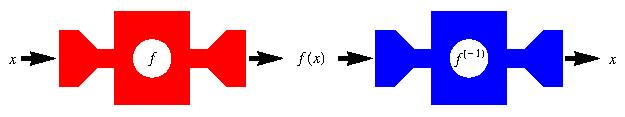
\includegraphics[height=2cm]{inverse-functions/pictures/07-01-machinesb.pdf}%
}
\uncover<6->{
Switch the roles of $x$ and $y$:
\[
\alert<handout:0| 8>{f^{-1}(x) = y} \qquad \Leftrightarrow \qquad \alert<handout:0| 9>{f(y) = x} .
\]
}
\uncover<7->{Therefore
\[
(f\circ f^{-1})(x) = f(\alert<handout:0| 8>{f^{-1}(x)}) = \uncover<8->{\alert<handout:0| 9>{f(\alert<handout:0| 8-9>{y})}} \uncover<9->{\alert<handout:0| 9>{ = x}.}
\]
}
\uncover<10->{
\psset{xunit=0.75cm, yunit=0.75cm}
\begin{pspicture}(-4, -2.5)(13,2.5)
\footnotesize
\rput[r] (-3.1, 0){$x$}
\psline[linewidth=3pt]{->}(-3,0)(-2.25,0)

\rput(0.25,0){
\fcMachine{$f^{-1}$}{blue}
}
\rput (4, 0){ $f^{-1}(x)$}
\psline[linewidth=3pt]{->}(2.75,0)(3.4,0)
\psline[linewidth=3pt]{->}(4.7,0)(5.25,0)
\rput(7.75,0){
\fcMachine{$f$}{red}
}
\rput (11.75, 0){$x$}
\psline[linewidth=3pt]{->}(10.25,0)(11,0)
\end{pspicture}
%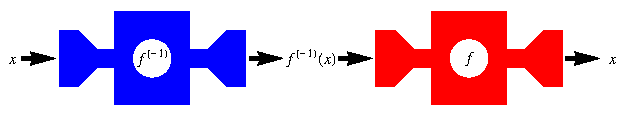
\includegraphics[height=2cm]{inverse-functions/pictures/07-01-machinesa.pdf}%
}
\end{frame}
% end module inverse-function-equations

% begin module inverse-function-solve-for
\begin{frame}
\frametitle{How to Find the Inverse of a One-to-one Function}
\begin{enumerate}
\item<1-| alert@3>  Write $y = f(x)$.
\item<1-| alert@4-5>  Solve this equation for $x$ in terms of $y$ (if possible).
\end{enumerate}
\uncover<2->{
\begin{example}%[Example 4, p. 388]
If $f(x) = x^3 + 2$, find a formula for $f^{-1}(y)$.
\begin{align*}
\uncover<3->{y} & \uncover<3->{=}  \uncover<3->{x^3 + 2}\\
\uncover<4->{x^3} & \uncover<4->{=}  \uncover<4->{y - 2}\\
\uncover<5->{\alert<handout:0| 6>{x}} & \uncover<5->{=}  \uncover<5->{\alert<6>{\sqrt[3]{y - 2}}}
\end{align*}
\uncover<6->{
Therefore \alert<6,8>{$x=f^{-1}(y) = \sqrt[3]{y - 2}$}.
}
\uncover<7->{
Sometimes we relabel $x$ and $y$ and write \only<7>{ $f^{-1}(x)=\sqrt[3]{x-2}$.} \only<8->{\color{gray!50} $f^{-1}(x)=\sqrt[3]{x-2}$.}
}
\uncover<8->{\alert<8>{
Whenever in doubt, do not relabel anything.
}}
\end{example}
}
\end{frame}
% end module inverse-function-solve-for

% begin module guess-and-check
\begin{frame}
\begin{example}[Guess and Check]
If $f(x) = 2x + \sin 2x + e^{x/2}$, find $f^{-1}(1)$.  
\begin{align*}
\uncover<2->{f\alert<handout:0| 2-3>{(\uncover<3-| handout:0>{0})}} & \uncover<2->{=}  \uncover<2->{2\alert<handout:0| 2-3>{(\uncover<3-| handout:0>{0})}  + \sin 2\alert<handout:0| 2-3>{(\uncover<3-| handout:0>{0})}  + e^{\alert<handout:0| 2-3>{(\uncover<3-| handout:0>{0})}/2} }\\ 
 & \uncover<2->{=}  \uncover<3-| handout:0>{0 + 0 + 1} \\
 & \uncover<2->{=}  \uncover<2->{1.} \\
\uncover<4->{\text{Therefore}\quad f^{-1}(1)} & \uncover<4->{=}  \uncover<4-| handout:0>{0.}
\end{align*}
\end{example}
\end{frame}
% end module guess-and-check

% begin module inverse-function-graph
\begin{frame}
\begin{tabular}{cc}
\psset{xunit=0.9cm, yunit=0.9cm}
\begin{pspicture}(-1.5,-1.5)(3.5,3.2)
\psaxes[ticks=none, labels=none]{<->}(0,0)(-1.5,-1.5)(3.4,3.1)
\fcLabels{3.4}{3.1}
\uncover<6->{
\psline(2.5, 1)(1, 2.5)
\psline(1.85, 1.65)(1.95, 1.75)(1.85, 1.85)
\psline(1.85, 1.85)(1.75, 1.95)(1.65, 1.85)

\psline(1.9875, 1.3125)(2.1875, 1.5125)
\psline(2.0625, 1.2375)(2.2625, 1.4375)
\psline(1.3125, 1.9875)(1.5125, 2.1875)
\psline(1.2375, 2.0625)(1.4375, 2.2625)

\psline[linecolor=blue](-1.35, -1.35)(2.8,2.8)
\rput[l](-1, -1.2){\footnotesize $y=x$}
}
\uncover<2->{
\fcFullDot{2.5}{1}
\rput[lt](2.6, 1.1){\footnotesize $(a,b)$}
}
\uncover<5->{
\fcFullDot{1}{2.5}
\rput[rb](0.9, 2.6){\footnotesize $(b,a)$}
}
\end{pspicture}
%\ \only<handout:0| -4>{%
%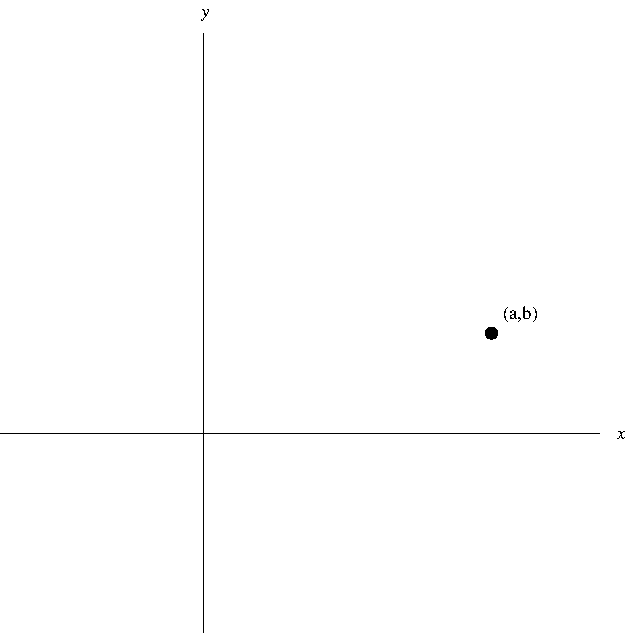
\includegraphics[height=4cm]{inverse-functions/pictures/07-01-reflecta.pdf}%
%}%
%\only<handout:0| 5>{%
%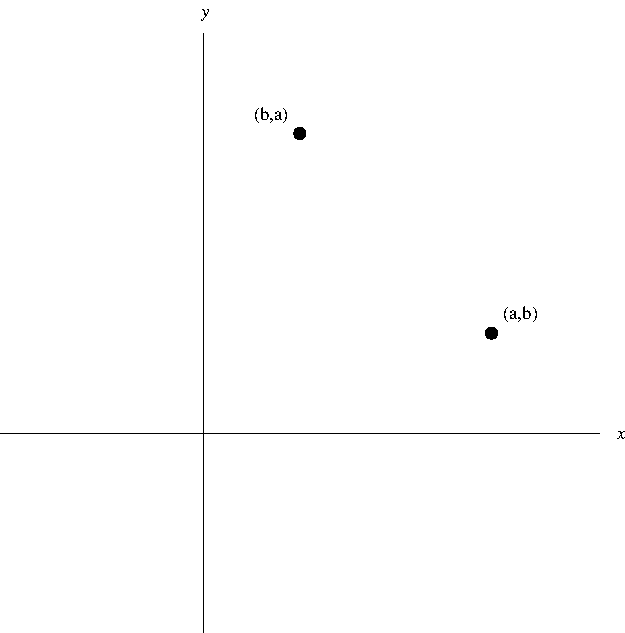
\includegraphics[height=4cm]{inverse-functions/pictures/07-01-reflectb.pdf}%
%}%
%\only<handout:1| 6->{%
%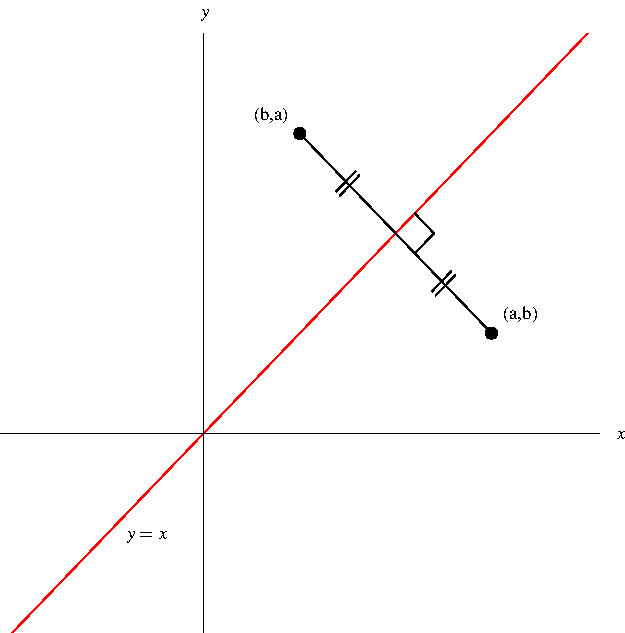
\includegraphics[height=4cm]{inverse-functions/pictures/07-01-reflectc.pdf}%
%}%
&%
\psset{xunit=0.9cm, yunit=0.9cm}
\begin{pspicture}(-1.55,-1.5)(3.5,3.2)
\psaxes[ticks=none, labels=none]{<->}(0,0)(-1.55,-1.5)(3.4,3.1)
\fcLabels{3.4}{3.1}
\uncover<7->{
\psline(0.75, 2.36359)(2.36359, 0.75)
\psline(1.65679, 1.65679)(1.55679, 1.75679)(1.45679, 1.65)
\psline(1.65679, 1.65679)(1.75679, 1.55679)(1.65679, 1.45679)
\fcFullDot{0.75}{2.36359}
\fcFullDot{2.36359}{0.75}

\psline[linecolor=blue](-1.35, -1.35)(2.8,2.8)
\rput[l](-1, -1.2){\footnotesize $y=x$}
\psplot[linecolor=red, plotpoints=1000]{-0.292893219}{3}{x 1 add ln  0.693147181 div 1 sub}
\rput[lb](0.9, 2.4){\footnotesize $y=f^{-1}(x)$}
%Function formula: 2^{1+x}-1
\psplot[linecolor=red, plotpoints=1000]{-1.5}{0.95}{-1 2 x 1 add exp add }
\psline[linecolor=blue](-1.4, -1.4)(2.9,2.9)
\rput[l](-1, -1.2){\footnotesize $y=x$}
\rput[tr](2.8, 0.4){\footnotesize $y=f(x)$}
}
\end{pspicture}
%\only<handout:0| -6>{%
%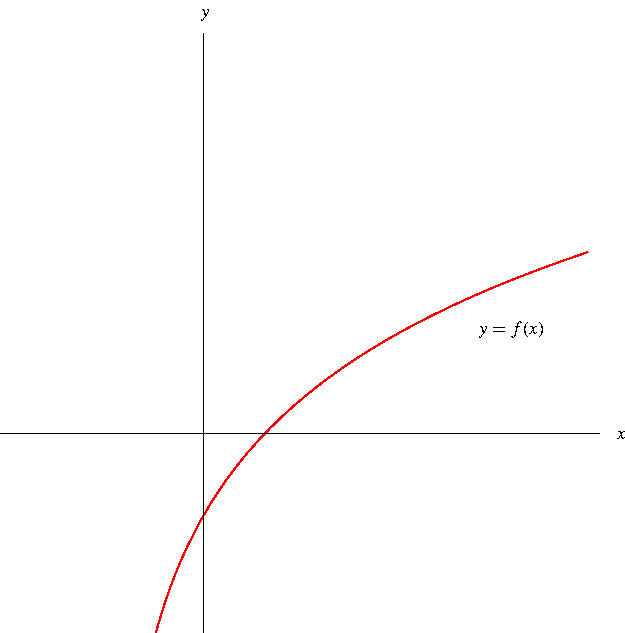
\includegraphics[height=4cm]{inverse-functions/pictures/07-01-reflect-functionb.pdf}%
%}%
%\only<handout:1| 7->{%
%\includegraphics[height=4cm]{inverse-functions/pictures/07-01-reflect-f unctiona.pdf}%
%}%
\end{tabular}

Interchanging $x$ and $y$ suggests relation between the graphs of $f^{-1}$ and $f$:
\begin{itemize}
\item<2->  Suppose $(a,b)$ is on the graph of $f$.
\item<3->  Then $f(a) = b$.
\item<4->  Then $f^{-1}(b) = a$.
\item<5->  Then $(b,a)$ is on the graph of $f^{-1}$.
\item<6->  $(b,a)$ is the reflection of $(a,b)$ in the line $y = x$.
\item<7->  Thus the graph of $f^{-1}$ is obtained by reflecting the graph of $f$ in the line $y = x$.
\end{itemize}
\end{frame}
% end module inverse-function-graph

% begin module inverse-function-ex5
\begin{frame}
\begin{example}%[Example 5, p. 388]
\begin{columns}[c]
\column{.5\textwidth}
\psset{xunit=0.5cm, yunit=0.5cm}
\begin{pspicture}(-5, -5)(5,5) 
\psframe*[linecolor=white](-5,-5)(5,5) 
\psaxes[ticks=none, labels=none]{<->}(0,0)(-4.5,-5)(4.5,5)
\psline(1, -0.1)(1, 0.1)
\rput[t](1, -0.2){\tiny$1$}
\psline(-1, -0.1)(-1, 0.1)
\psline(-0.1, 1)(0.1, 1)
\rput[br](-0.2, 1){\tiny$1$}
\psline(-0.1, -1)(0.1, -1)
\uncover<3>{
%Function formula: sqrt{}(- (x)) 
\psplot[linecolor=red, plotpoints=1000]{-4.5}{0}{x -1 mul sqrt }
\rput(-2, 2.2){\tiny$y=\sqrt{-x}$}
}
\uncover<4->{
%Function formula: sqrt{}(- (x)) 
\psplot[linecolor=gray, plotpoints=1000]{-4.5}{0}{x -1 mul sqrt }
\rput(-2, 2.2){\color{gray}\tiny$y=\sqrt{-x}$}
}
\uncover<2>{
 %Function formula: sqrt{}(x) 
\psplot[linecolor=red, plotpoints=1000]{0}{4.5}{x sqrt } 
\rput(2.4, 1){\tiny $y=\sqrt{x}$}
}
\uncover<3->{
 %Function formula: sqrt{}(x) 
\psplot[linecolor=gray, plotpoints=1000]{0}{4.5}{x sqrt } 
\rput(2.4, 1){\color{gray}\tiny $y=\sqrt{x}$}
}
\uncover<4>{
%Function formula: sqrt{}(- (x)-1) 
\psplot[linecolor=red, plotpoints=1000]{-4.5}{-1}{-1 x -1 mul add sqrt }
\rput[r](-2.3, 0.55){\tiny$y=f(x)$}
}
\uncover<5->{
%Function formula: sqrt{}(- (x)-1) 
\psplot[linecolor=gray, plotpoints=1000]{-4.5}{-1}{-1 x -1 mul add sqrt }
\rput[r](-2.3, 0.55){\color{gray}\tiny$y=f(x)$}
}

\uncover<5>{
%Function formula: - ((x)^{2})-1 
\psplot[linecolor=red, plotpoints=1000]{0}{2}{-1 x 2 exp -1 mul add } 
\rput[l](1.3, -2){\tiny$y=f^{-1}(x)$}
\psline[linecolor=blue, linestyle=dashed] (-4.5, -4.5)(4.5, 4.5)
\rput[tl](-3, -3.2){\tiny $y=x$}
}
\end{pspicture} 
%\ \only<handout:0| -1>{%
%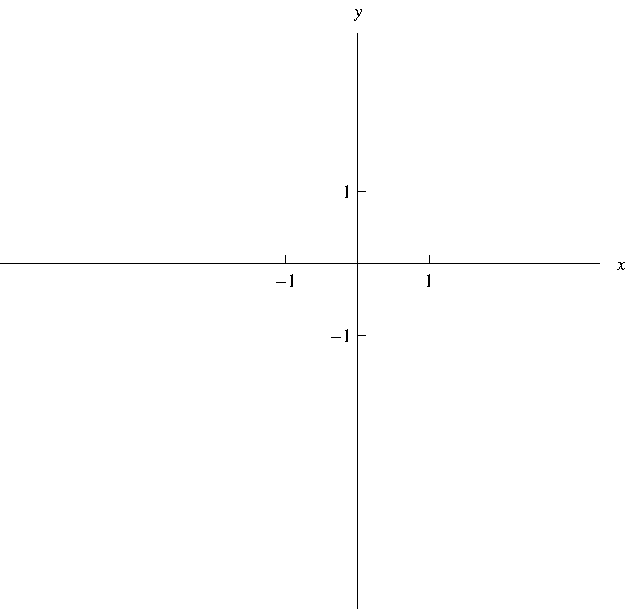
\includegraphics[height=4.5cm]{inverse-functions/pictures/07-01-ex5a.pdf}%
%}%
%\only<handout:0| 2>{%
%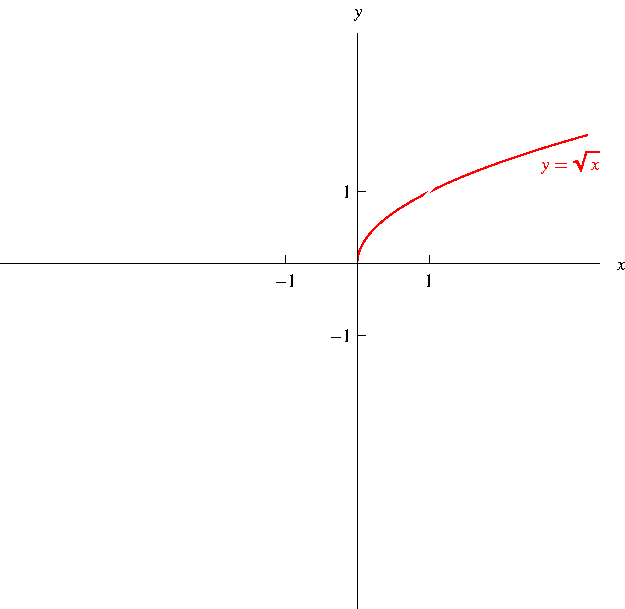
\includegraphics[height=4.5cm]{inverse-functions/pictures/07-01-ex5b.pdf}%
%}%
%\only<handout:0| 3>{%
%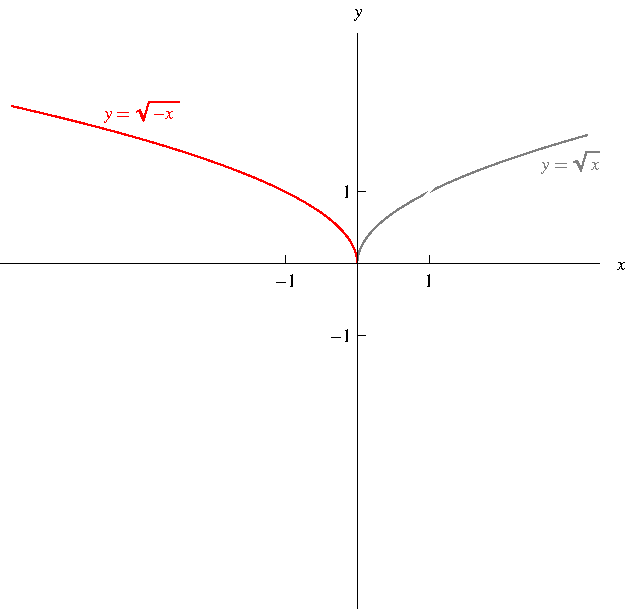
\includegraphics[height=4.5cm]{inverse-functions/pictures/07-01-ex5c.pdf}%
%}%
%\only<handout:0| 4>{%
%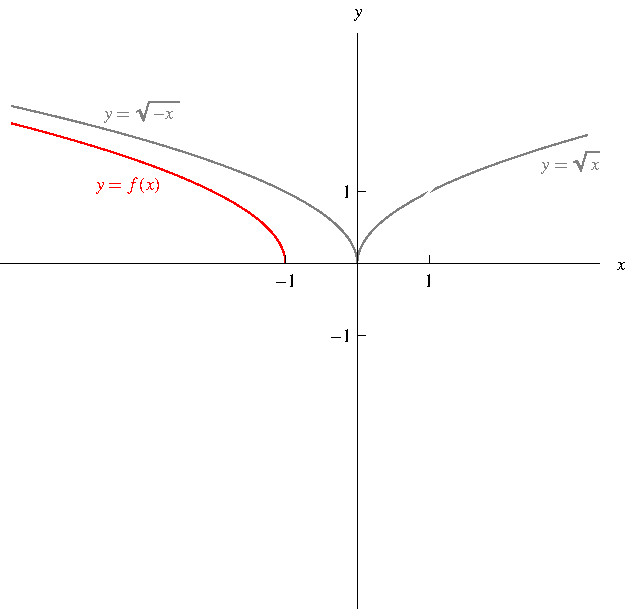
\includegraphics[height=4.5cm]{inverse-functions/pictures/07-01-ex5d.pdf}%
%}%
%\only<handout:1| 5->{%
%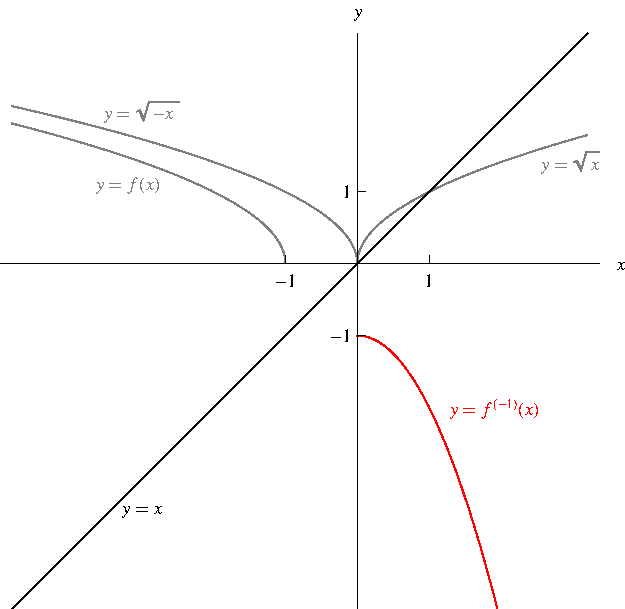
\includegraphics[height=4.5cm]{inverse-functions/pictures/07-01-ex5e.pdf}%
%}%

\column{.5\textwidth}
Sketch the graph of $f(x) = \sqrt{-x - 1}$ and its inverse function.
\end{columns}
\begin{itemize}
\item<2->  First draw the graph of $y = \sqrt{x}$.
\item<3->  $y = \sqrt{-x}$ is the reflection of $y = \sqrt{x}$ in the $y$-axis.
\item<4->  $y = f(x) = \sqrt{-x - 1}$ is the shift of $y = \sqrt{-x}$ one unit to the left.
\item<5->  $y = f^{-1}(x)$ is the reflection of $y = f(x)$ across the line $y = x$.
\end{itemize}
\end{example}
\end{frame}
% end module inverse-function-ex5
% begin module inverse-function-solve-for
\begin{frame}
%\frametitle{Inverse of a ne-to-one Function}
\begin{example}[\uncover<handout:2|16->{\alert<handout:0| 16,17>{What if we change the problem to $x\leq -\frac{2}3$?}}]
Given: $\alert<handout:0| 2>{f(x) =  3x^2+4x-7}$ \alert<handout:0| 3,16,17>{with domain $x\only<handout:1|1-16| handout:1>{\geq}\only<handout:2|17->{\leq} -\frac{2}{3}$}.  Find $f^{-1}(x)$.
\begin{columns}
\column{0.4\textwidth}
\psset{xunit=0.35cm, yunit=0.35cm}
\begin{pspicture}(-9,-9)(5,5)
\psframe*[linecolor=white](-9,-9)(5,5)
\tiny
\psaxes[ticks=none, labels=none]{<->}(0,0)(-9,-9)(4.7,4.7)
\uncover<2-16| handout:1>{ %
\psplot[linecolor=\fcColorGraph, plotpoints=1000] {-0.66}{1.401612274}{x 2 exp 3 mul x 4 mul add -7 add }
}
\uncover<handout:2|17->{ %
\psplot[linestyle=dashed, linecolor=gray!50, plotpoints=1000]{-0.66}{1.401612274}{x 2 exp 3 mul x 4 mul add -7 add }
}
\uncover<handout:2|2,17>{ %
\psplot[linecolor=\fcColorGraph, plotpoints=1000]{-2.7349}{-0.67}{x 2 exp 3 mul x 4 mul add -7 add }
}
\uncover<3-16| handout:1>{ %
\psplot[linestyle=dashed, linecolor=gray!50, plotpoints=1000] {-2.7349}{-0.67}{x 2 exp 3 mul x 4 mul add -7 add }
}
\uncover<14->{
\psline[linecolor=blue, linestyle=dashed](-6.5, -6.5)(4.5,4.5)
}
\uncover<15-16| handout:1>{
\psplot[linecolor=red, plotpoints=1000]{-8.33333}{4.5}{-0.666667 25 x 3 mul add sqrt 0.333333 mul add }
}
\uncover<handout:2|17->{
\psplot[linestyle=dashed, linecolor=gray!50, plotpoints=1000] {-8.33333}{4.5}{-0.666667 25 x 3 mul add sqrt 0.333333 mul add }
}
\uncover<handout:1|15-16>{
\psplot[linecolor=gray!50, linestyle=dashed, plotpoints=1000] {-8.33333}{4.5}{-0.666667 25 x 3 mul add sqrt -0.333333 mul add }
}
\uncover<handout:2|17->{
\psplot[linecolor=\fcColorGraph, plotpoints=1000] {-8.33333}{4.5}{-0.666667 25 x 3 mul add sqrt -0.333333 mul add }
}
\uncover<15-16| handout:1>{\rput[lb](-6, 1){$y=f^{-1}(x)$}}
\uncover<11->{\rput (-3.5, -8 ){$\left(-\frac{2}{3}, -\frac{25}{3}\right)$}}
\uncover<2-16| handout:1>{\rput[tl](1.8, 4.45){$y=f(x)$}}
\uncover<14->{\rput[l] (-7.8, -2.2 ){$\left(-\frac{25}{3}, -\frac{2}{3}\right)$}}
\uncover<handout:2|17->{\rput[rt](4.5, -3){$y=f^{-1}(x)$}}
\uncover<handout:2|17>{ \rput[tr](-3, 4.5){$y=f(x)$}}
\uncover<14->{\fcFullDot{-8.33333}{-0.666667}}
\fcFullDot{-0.666667}{-8.33333}
\end{pspicture}
\uncover<13->{Final }\uncover<12->{answer}\uncover<13->{, \alert<handout:0| 13>{relabelled}:}
\[
\uncover<12->{
f^{-1}(\only<12| handout:0>{y}\only<13->{\alert<handout:0| 13>{x}} )=-\frac{2}{3} \only<1-16| handout:1>{+} \only<handout:2|17->{\alert<handout:0| 17>{-}} \frac{\sqrt{25 +3\only<12| handout:0>{y} \only<13->{\alert<handout:0| 13>{x}}\phantom{y} }}{3}\quad.
}
\]

\column{0.6\textwidth}

\[\begin{array}{rcl}
\uncover<4->{3x^2+4x-7&=&y } \\
\uncover<4->{\alert<handout:0| 7>{3}x^2+\alert<handout:0| 6>{4}x+\alert<handout:0| 8>{(-7-y)}&=&0 }
\end{array}
\]
\uncover<5->{That's \alert<handout:0| 6,7,8>{a quadratic equation in $x$}. Solve:}
\[\begin{array}{l}
\uncover<5->{
\phantom{=}\displaystyle \frac{-\alert<handout:0| 6>{4} \pm \sqrt{\alert<handout:0| 6>{4}^2-4\cdot\alert<handout:0| 7>{3}\cdot\alert<handout:0| 8>{(-y-7)} }}{2\cdot\alert<handout:0| 7>{3}} \\
%~&=& \frac{-2 \pm \sqrt{25+3y}}{3}\\
}
\\
\uncover<9->{=\displaystyle-\frac{2 \pm \sqrt{25+3y}}{3}=} \uncover<10->{\displaystyle-\frac{2}3 \pm \frac{\sqrt{25+3y}}{3}\quad .}
\end{array}
\]
\uncover<11->{
We are given $x\only<11-16| handout:1>{\geq} \only<handout:2|17->{\alert<handout:0| 17>{\leq}}-\frac{2}3 $, therefore $x=-\frac{2}{3}\only<11-16| handout:1>{ +} \only<handout:2|17->{\alert<handout:0| 17>{-}} \frac{\sqrt{25+3y}}{3}=f^{-1}(y)$.
}
\end{columns}
\vspace{-10pt}
\end{example}
\end{frame}
% end module inverse-function-solve-for

% end lecture

% begin lecture
\lect{February 28, 2014}{Lecture 10}{10}
\section{Logarithmic Functions}
% begin module logarithm-def
\begin{frame}
\frametitle{Logarithmic Functions}
\begin{columns}[c]
\column{.3\textwidth}
\psset{xunit=0.7cm, yunit=0.7cm}
\begin{pspicture}(-5, -5)(5,5) 
\psframe*[linecolor=white](-5,-5)(5,5) 
\psaxes[ticks=none, labels=none]{<->}(0,0)(-2,-2.1)(4.2, 4.2)
\psline(-0.1, 1)(0.1,1)
\rput[r](-0.2, 1){\footnotesize$1$}
\rput(0.9, 3){\footnotesize$y=a^x$}
%Function formula: 2^{x} 
\psplot[linecolor=red, plotpoints=1000]{-2}{2}{2 x exp }
\uncover<8->{
\psplot[linecolor=red, plotpoints=1000]{0.25}{4}{x ln 0.693147181 div }
\psline[linestyle=dashed, linecolor=blue](-1.9, -1.9)(4,4) 
\rput[tl](2, 0.7){\footnotesize$y=\log_ax$}
}
\end{pspicture} 
%\ \only<handout:0| -7>{%
%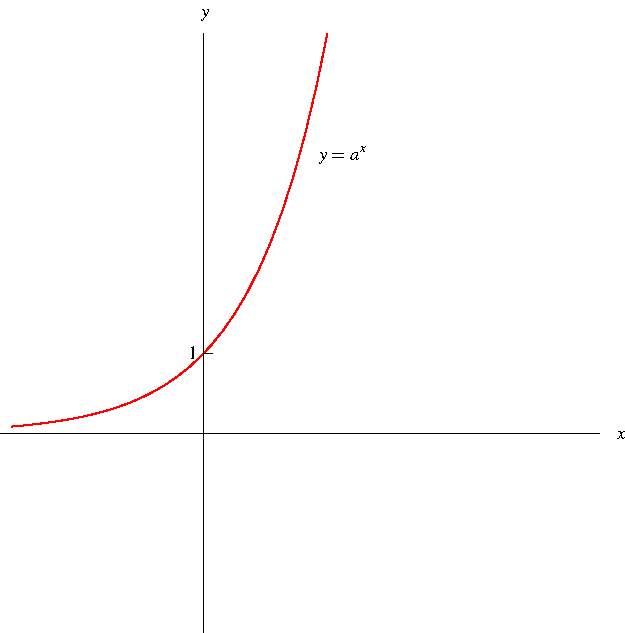
\includegraphics[height=4cm]{logarithms/pictures/07-03-logandexpa.pdf}%
%}%
%\only<8->{%
%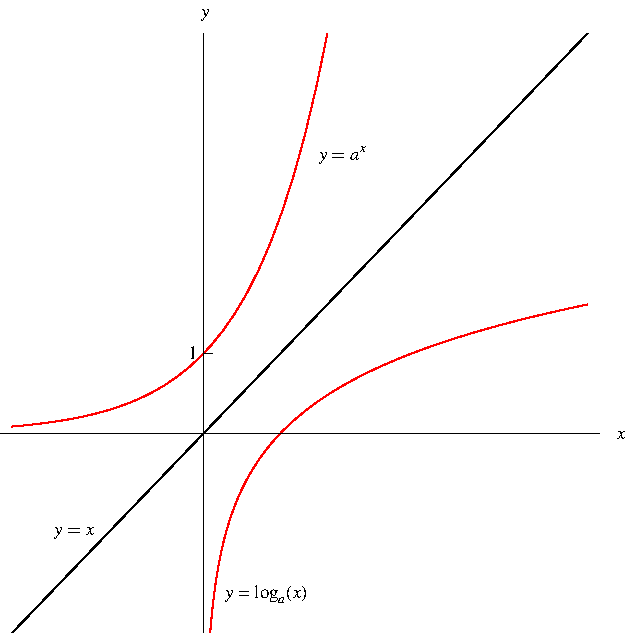
\includegraphics[height=4cm]{logarithms/pictures/07-03-logandexpb.pdf}%
%}%
\column{.7\textwidth}
\begin{itemize}
\item  Suppose $a > 0$, $a\neq 1$.
\item<2->  Let $f(x) = a^x$.
\item<3->  Then $f$ is either increasing or decreasing.
\item<4->  Therefore $f$ is one-to-one.
\item<5->  Therefore $f$ has an inverse function, $f^{-1}$.
\item<7->  The graph shows $y = a^x$ for $a > 1$.
\item<8->  The graph of $y = \log_a x$ is the reflection of this in the line $y = x$.
\end{itemize}
\end{columns}
\uncover<6->{%
\begin{definition}[$\log_a x$]
The inverse function of $f(x) = a^x$ is called the logarithmic function with base $a$, and is written $\log_a x$.  It is defined by the formula
\[
\log_a x = y \qquad \Leftrightarrow \qquad a^y = x .
\]
\end{definition}
}%
\end{frame}
% end module logarithm-def

% begin module logarithm-def-ex1
\begin{frame}
If $x > 0$, then $\log_a x$ is the exponent to which the base $a$ must be raised to give $x$.
\begin{example}%[Example 1, p. 405]
Evaluate:
\begin{enumerate}
\item<1-| alert@2-3> $\log_3 81 =$ \uncover<3->{$4$ because $3^4 = 81$.}
\item<1-| alert@4-5> $\log_{25} 5 =$ \uncover<5->{$\frac{1}{2}$ because $25^{1/2} = 5$.}
\item<1-| alert@6-7> $\log_{10} 0.001 =$ \uncover<7->{$-3$ because $10^{-3} = 0.001$.}
\end{enumerate}
\end{example}
\end{frame}
% end module logarithm-def-ex1

% begin module log-and-exp
\begin{frame}
\begin{columns}[c]
\column{.6\textwidth}
\psset{xunit=1cm, yunit=1cm}
\begin{pspicture}(-5, -5)(5,5) 
\psframe*[linecolor=white](-5,-5)(5,5) 
\psaxes[ticks=none, labels=none]{<->}(0,0)(-2,-2.1)(4.2, 4.2)
\psline(-0.1, 1)(0.1,1)
\rput[r](-0.2, 1){\footnotesize$1$}
\rput(0.9, 3){\footnotesize$y=a^x$}
%Function formula: 2^{x} 
\psplot[linecolor=red, plotpoints=1000]{-2}{2}{2 x exp }
\psplot[linecolor=red, plotpoints=1000]{0.25}{4}{x ln 0.693147181 div }
\psline[linestyle=dashed, linecolor=blue](-1.9, -1.9)(4,4) 
\rput[tl](2, 0.7){\footnotesize$y=\log_ax$}
\rput[tl](-1, -1.1){\footnotesize$y=x$}
\end{pspicture} 
%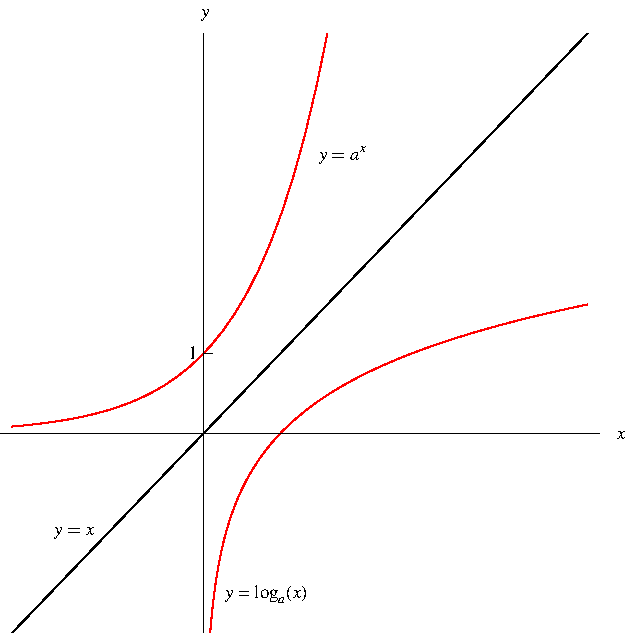
\includegraphics[height=7cm]{logarithms/pictures/07-03-logandexpb.pdf}%
\column{.4\textwidth}
\begin{itemize}
\item  Suppose $a > 1$.
\item<2-| alert@3-4>  Domain of $a^x$: \uncover<4->{$\mathbb{R}$.}
\item<2-| alert@5-6>  Range of $a^x$: \uncover<6->{$(0, \infty )$.}
\item<2-| alert@7-8>  Domain of $\log_a x$: \uncover<8->{$(0, \infty )$.}
\item<2-| alert@9-10>  Range of $\log_a x$: \uncover<10->{$\mathbb{R}$.}
\item<11->  $\log_a (a^x) = x$ for $x\in \mathbb{R}$.
\item<11->  $a^{\log_a x} = x$ for $x > 0$.
%\item<12-| alert@13-14>  $\lim_{x\rightarrow \infty}\log_a x = \uncover<14->{\infty .}$
%\item<12-| alert@15-16>  $\lim_{x\rightarrow 0^+}\log_a x = \uncover<16->{-\infty .}$
\end{itemize}
\end{columns}
\end{frame}
% end module log-and-exp

% begin module logarithm-graphs
\begin{frame}
\begin{center}
Graphs of various logarithmic functions with $a > 1$
\psset{xunit=1cm, yunit=1cm}
\begin{pspicture}(-0.5,-4.5)(7.5,3.2)
\psaxes[ticks=none, labels=none]{<->}(0,0)(-0.5,-4.5)(7.5,3.2)
\psline(1,-0.1)(1,0.1)
%Function formula: ln(x)/ln(2)
\psplot[linecolor=red, plotpoints=1000]{0.044194174}{7.5}{x ln 0.693147181 div}
\rput[r](3, 1.8){\footnotesize $y=log_2 x$}
\uncover<2->{
%Function formula: ln{x}/ln(3) 
\psplot[linecolor=black, plotpoints=1000]{0.007127781}{7.5}{x ln 1.098612289 div}
\rput[l](3.6, 1.6 ){\footnotesize $y=log_3 x$}
}
\uncover<3->{
%Function formula: ln{x}/ln(5) 
\psplot[linecolor=blue, plotpoints=1000]{0.000715542}{7.5}{x ln 1.609437912 div}
\rput[l](3.7, 1.1){\footnotesize $y=log_5 x$}
}
\uncover<4->{
%Function formula: ln{x}/ln(5) 
\psplot[linecolor=green, plotpoints=1000]{0.000031623}{7.5}{x ln 2.302585093 div}
\rput[tl](3.6, 0.6){\footnotesize $y=log_{10} x$}
}
%\rput(6, 1){\color{red!1} .}
\end{pspicture} 
%\ \only<handout:0| -1>{%
%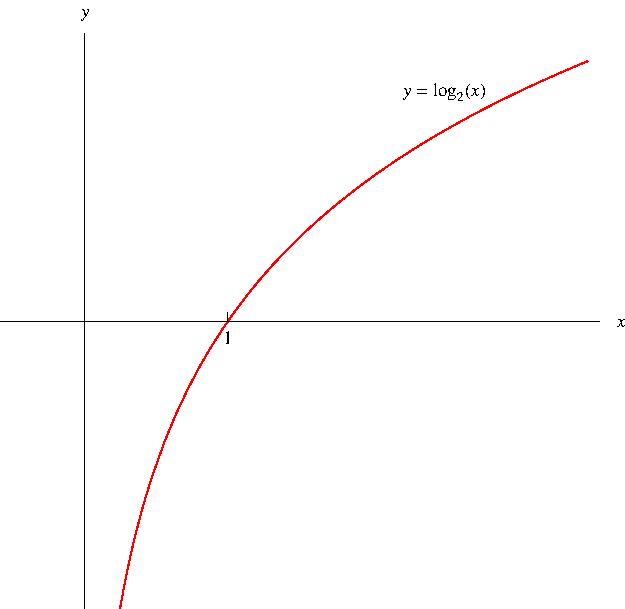
\includegraphics[height=6cm]{logarithms/pictures/07-03-manylogsa.pdf}%
%}%
%\only<handout:0| 2>{%
%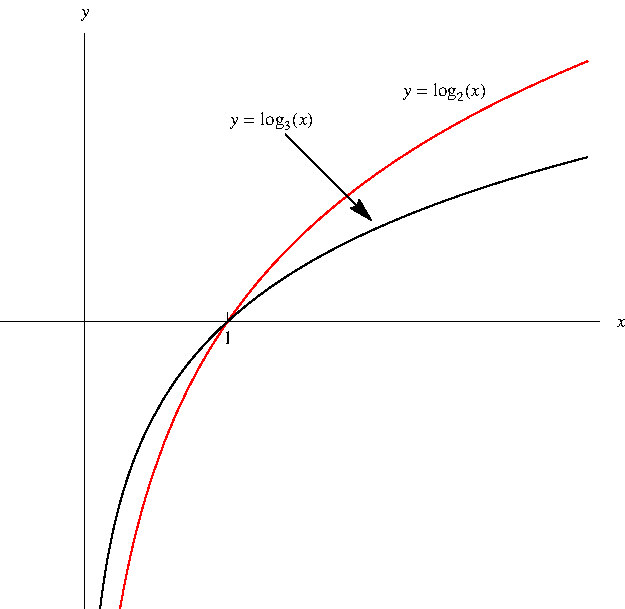
\includegraphics[height=6cm]{logarithms/pictures/07-03-manylogsb.pdf}%
%}%
%\only<handout:0| 3>{%
%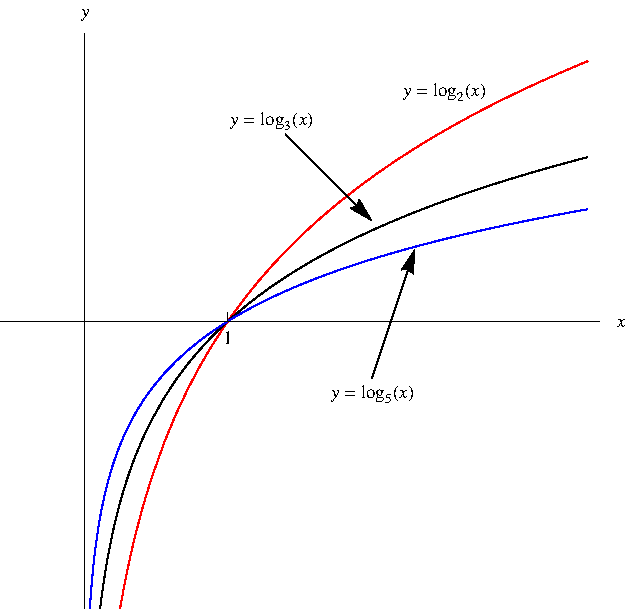
\includegraphics[height=6cm]{logarithms/pictures/07-03-manylogsc.pdf}%
%}%
%\only<4->{%
%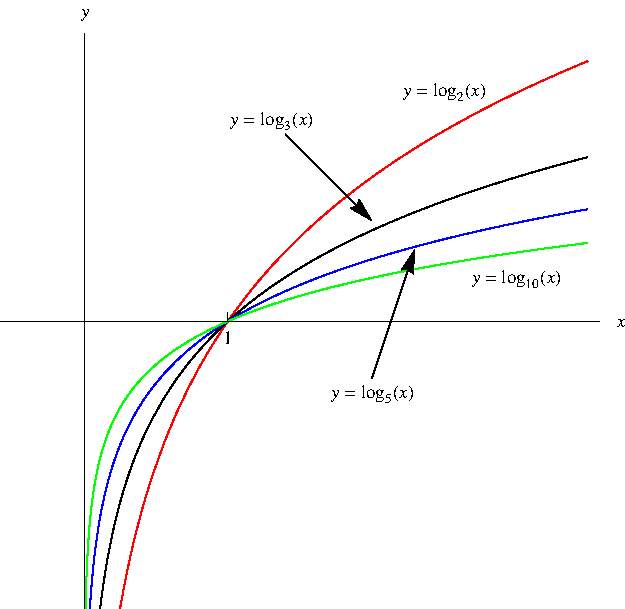
\includegraphics[height=6cm]{logarithms/pictures/07-03-manylogsd.pdf}%
%}%
\pause\pause\pause
\end{center}
\end{frame}
% end module logarithm-graphs
% begin module logarithm-properties
\begin{frame}
\begin{theorem}[Properties of Logarithmic Functions]
If $a > 1$, the function $f(x) = \log_a x$ is a one-to-one, continuous, increasing function with domain $(0, \infty )$ and range $\mathbb{R}$.  If $x, y, a, b > 0$ and $r$ is any real number, then
\begin{enumerate}
\item  $\log_a (xy) = \log_a x + \log_a y$.
\item  $\log_a \left( \frac{x}{y}\right) = \log_a x - \log_a y$.
\item  $\log_a (x^r) = r\log_a x$.
\item  $\log_{a}(x)=\log_b x \log_{a} b=\frac{\log_b x}{\log_{b} a}=  \frac{\ln x}{\ln a}$.
\end{enumerate}
\end{theorem}

\end{frame}
% end module logarithm-properties

% begin module logarithm-properties-ex2
\begin{frame}
\begin{example}%[Example 2, p. 406]
Use the properties of logarithms to evaluate the following:
\begin{columns}[t]
\column{.5\textwidth}
\begin{align*}
& \invisible{=} \log_4 2 + \log_4 32 \\
&\uncover<2->{=}  \uncover<2->{\log_4 (2\cdot 32 )} \\
&\uncover<3->{=}  \uncover<3->{\log_4 (64)} \\
&\uncover<4->{=}  \uncover<4->{3} \\
& \uncover<4->{\text{(because $4^3 = 64$.)}}
\end{align*}
\column{.5\textwidth}
\begin{align*}
& \invisible{=} \log_2 80 - \log_2 5 \\
&\uncover<5->{=}  \uncover<5->{\log_2 \left( \frac{80}{5}\right) } \\
&\uncover<6->{=}  \uncover<6->{\log_2 (16)} \\
&\uncover<7->{=}  \uncover<7->{4} \\
& \uncover<7->{\text{(because $2^4 = 16$.)}}
\end{align*}
\end{columns}
\end{example}
\end{frame}
% end module logarithm-properties-ex2

\subsection{Natural Logarithms}
% begin module natural-logarithm-def
\begin{frame}
\frametitle{Natural Logarithms}
\begin{definition}[$\ln x$]
The logarithm with base $e$ is called the natural logarithm, and has a special notation:
\[
\log_e x = \ln x .
\]
\end{definition}
\begin{columns}[c]
\column{.5\textwidth}
\psset{xunit=0.6cm, yunit=0.6cm}
\begin{pspicture}(-4.2,-4.2)(4.2, 4.2)
\psframe*[linecolor=white](-4.2,-4.2)(4.2, 4.2)
\psaxes[ticks=none, labels=none]{<->}(0,0)(-4.2,-4.2)(4.2, 4.2)
\psline(-0.1, 1)(0.1,1)
\rput[r](-0.2, 1){\footnotesize$1$}
\psline(1, -0.1)(1,0.1)
\rput[t](1, -0.2){\footnotesize$1$}
\rput[l](1.3, 3.2){\footnotesize$y=e^x$}
%Function formula: 2^{x} 
\psplot[linecolor=red, plotpoints=1000]{-4}{1.386294361}{2.718281828 x exp }
\psplot[linecolor=red, plotpoints=1000]{0.018315639}{4}{x ln}
\psline[linestyle=dashed, linecolor=blue](-4, -4)(4,4) 
\rput[tl](2, 0.7){\footnotesize$y=\ln x$}
\rput[tl](-2, -2.3){\footnotesize$y=x$}
\end{pspicture} 
%\ 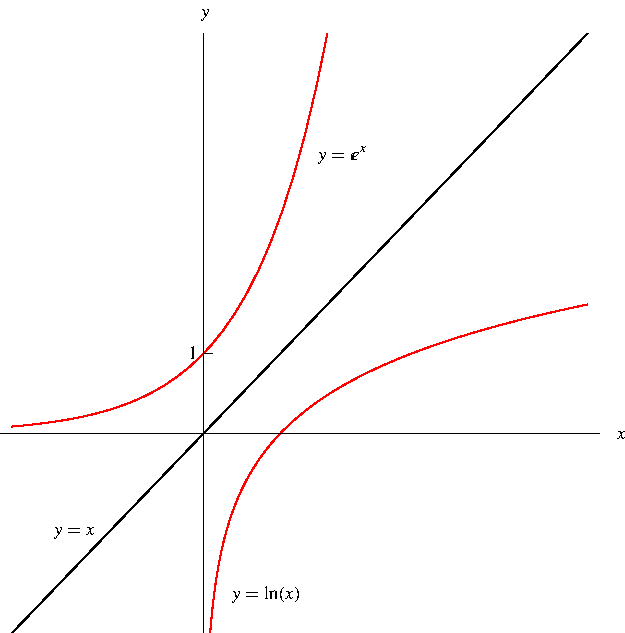
\includegraphics[height=5cm]{logarithms/pictures/07-03-natlog.pdf}%
\column{.5\textwidth}
\begin{itemize}
\item<2->  $\ln x = y \qquad \Leftrightarrow \qquad e^y = x$ .
\item<3->  $\ln (e^x ) = x$ for $x\in \mathbb{R}$.
\item<4->  $e^{\ln x}  = x$ for $x > 0$.
\end{itemize}
\end{columns}
\end{frame}
% end module natural-logarithm-def

% begin module natural-logarithm-def-ex5
\begin{frame}
\begin{example}
Solve the equation.
\[\begin{array}{rclll}
\displaystyle e^{5-3x} & =&  10 \uncover<2->{&&\text{apply }\alertNoH{2}{\ln}}\\
\uncover<2-| handout:0>{\displaystyle  \alertNoH{2,3}{\ln} ({\alertNoH{3}{e}}^{5-3x}) & =&\displaystyle  \uncover<2-| handout:0>{\alertNoH{2}{\ln} 10} } \\
\uncover<3-| handout:0>{\displaystyle \alertNoH{4}{5-}3x} & \uncover<3->{=}& \displaystyle  \uncover<3-| handout:0>{\ln 10} \\
\displaystyle \uncover<4-| handout:0>{\alertNoH{5}{3}x} & \uncover<4->{=}& \displaystyle  \uncover<4-| handout:0>{\alertNoH{4}{5-}\ln 10} \\
\displaystyle \uncover<5->{x} & \uncover<5->{=}& \displaystyle \uncover<5-| handout:0>{\frac{5-\ln 10}{\alertNoH{5}{3}}} \\
\uncover<6->{\text{Calculator:}\quad x & \approx& 0.8991.}
\end{array}
\]
\end{example}
\end{frame}
% end module natural-logarithm-def-ex5

% begin module natural-logarithm-def-ex5
\begin{frame}
\begin{example}
\text{Solve the equation}
\[
e^{2x}-3e^x-4 =  0
\]
\uncover<2->{Set $e^x=u$. \uncover<3->{Then $\alertNoH{3,4}{e^{2x}=\uncover<4->{u^2}} $.} }
\begin{align*}
\uncover<5->{u^2-3u-4 &=0} \\
\uncover<6->{\alertNoH{6,7}{\left( \uncover<7->{u-4}\right)\left(\uncover<7->{u+1}\right)} &=0}
\end{align*}
\begin{align*}
\uncover<8->{ u=4 & &\text{or} & & u=-1}\\
\uncover<8->{e^x=4  & &\text{or} & & e^x=-1}\\
\uncover<9->{x=\ln 4} \uncover<10->{& &\text{or} & &  \text{no real solution}}\\
\uncover<11->{x\approx 1.386294361 }
\end{align*}
\end{example}
\end{frame}
% end module natural-logarithm-def-ex5

% begin module natural-logarithm-def-ex5
\begin{frame}
\begin{example}
\text{Solve the equation} 
\[  
4^{x+1}+2^{x+2}-3 =  0
\]
\uncover<2->{Set $\alert<2,3>{u= \uncover<3->{2^x}}$.} \uncover<5->{Then $\alert<5,6>{4^{x+1}=\uncover<6->{4u^2} }$,} 
\uncover<7->{$\alert<7,8>{2^{x+2}=\uncover<8->{4u} }$.} 
\begin{align*}
\uncover<9->{4u^2+4u-3 &=0} \\
\uncover<10->{\alert<10,11>{4\left( \uncover<11->{u-\frac{3}2}\right)\left(\uncover<11->{u+\frac12}\right)} &=0}
\end{align*}
\begin{align*}
\uncover<12->{u=\frac32 & &\text{or} & & u=-\frac12}\\
\uncover<12->{2^x=\frac32  & &\text{or} & & 2^x=-\frac12}\\
\uncover<13->{
x=\log_2 \left(\frac32\right) =}\uncover<15->{ \frac{\alert<15,16>{\ln \uncover<16->{\frac32}} }{\alert<15,16>{\ln \uncover<16->{2}}} \uncover<17->{\approx 0.584962501} \quad  }  \uncover<14->{& &\text{or} & & \text{no real solution}}
\end{align*}
\end{example}
\end{frame}
% end module natural-logarithm-def-ex5

% begin module natural-logarithm-def-ex8
\begin{frame}
\begin{example}%[Example 8, p. 408]
Draw the graph of $y = \ln (x - 2) -1$.
\begin{columns}[c]
\column{.55\textwidth}
\psset{xunit=1cm, yunit=1cm}
\begin{pspicture}(-5, -5)(5,5) 
\psframe*[linecolor=white](-5,-5)(6,6) 
\psaxes[ticks=none, labels=none]{<->}(0,0)(-0.5,-3)(6,2.5)
\psLabelXOne
\psLabelYOne
\uncover<2>{
\psplot[linecolor=red, plotpoints=1000]{0.049787068}{6}{x ln}
\rput[lb](0.6, 0.8){\footnotesize $y=\ln(x)$}
}
\uncover<3->{
\psplot[linecolor=gray, plotpoints=1000]{0.049787068}{6}{x ln}
\rput[lb](0.6, 0.8){\color{gray}\footnotesize $y=\ln(x)$}
}
\uncover<3>{
\psplot[linecolor=red, plotpoints=1000]{2.049787068}{6}{x -2 add ln}
\rput[lb](4, 0.3){\footnotesize$y=\ln(x-2)$}
}
\uncover<4->{
\psplot[linecolor=gray, plotpoints=1000]{2.049787068}{6}{x -2 add ln}
\rput[lb](4, 0.3){\color{gray}\footnotesize$y=\ln(x-2)$}
}
\uncover<3->{
\psline[linestyle=dashed, linecolor=blue](2, -3)(2, 2.5)
\rput[l](2.1, 2){\footnotesize$x=2$}
}
\uncover<4->{
\psplot[linecolor=red, plotpoints=1000]{2.135335283}{6}{x -2 add ln -1 add}
\rput(4, -2.3){\footnotesize$y=\ln(x-2)-1$}
}

\end{pspicture} 
%\ \only<handout:0| -1>{%
%\includegraphics[height=6cm]{logarithms/pictures/07-03-ex8a.pdf}%
%}%
%\only<handout:0| 2>{%
%\includegraphics[height=6cm]{logarithms/pictures/07-03-ex8b.pdf}%
%}%
%\only<3->{%
%\includegraphics[height=6cm]{logarithms/pictures/07-03-ex8c.pdf}%
%}%
\column{.45\textwidth}
\begin{itemize}
\item<2-> Graph $y=\ln(x)$ assumed given.
\item<3-> $f(x-2)$ shifts graph $2$ units to the right.
\item<4-> $g(x)-1$ shifts graph $1$ unit down.
\end{itemize}
\end{columns}
\end{example}
\end{frame}
% end module natural-logarithm-def-ex8

% begin module inverse-function-solve-for
\begin{frame}
%\frametitle{Inverse of a ne-to-one Function}
\vskip -0.2cm
\begin{example}
\begin{columns}
\column{0.35\textwidth}
Find $f^{-1}(x)$ for $\displaystyle f(x) = \frac{e^x-e^{-x}}{e^x+e^{-x}}  $. 
\uncover<18->{\alertNoH{18}{$f=\tanh$ = hyperbolic tangent function.}}

\psset{xunit=0.6cm, yunit=0.6cm}
\begin{pspicture}(-3.05,-3.1)(3.15,3.2)
\psframe*[linecolor=white](-3.05,-3.1)(3.15,3.2)
\tiny
\psaxes[ticks=none, labels=none]{<->}(0,0)(-3.05,-3.1)(3.05,3.1)
\fcLabels{3.05}{3.1}
%Function formula: (679570457/250000000^{x}- (679570457/250000000^{- (x)}))/(679570457/250000000^{- (x)}+679570457/250000000^{x})
\uncover<1-16>{
\rput(-2,-0.5){$y=f(x)$}
\psplot[linecolor=\fcColorGraph, plotpoints=1000]{-3}{3}{2.71828 x -1 mul exp -1 mul 2.71828 x exp add 2.71828 x exp 2.71828 x -1 mul exp add div }
}
\uncover<17->{
\rput(-2,-0.5){$y=f(x)$}
\psplot[linecolor=gray!50, plotpoints=1000]{-3}{3}{2.71828 x -1 mul exp -1 mul 2.71828 x exp add 2.71828 x exp 2.71828 x -1 mul exp add div }
}
%Function formula: 1/2 (\ln{}((1+x)/(1- (x))))
\uncover<17->{
\psline[linestyle=dashed, linecolor=blue](-3, -3)(3,3)
\rput[tl](1.1,2.5){$y=f^{-1}(x)$}
\psplot[linecolor=\fcColorGraph, plotpoints= 1000]{ -0.994}{ 0.994 }{x 1 add x -1 mul 1 add div ln 0.5 mul }
}
\end{pspicture}
\uncover<17->{Final }\uncover<16->{answer}\uncover<17->{, \alertNoH{17}{relabeled}:}
$\displaystyle 
\uncover<16->{
f^{-1}( \only<handout:0|16>{y}\only<17->{\alertNoH{17}{x}} )=\frac12\ln\left( \frac{1+\only<handout:0|16>{y} \only<17->{ \alertNoH{17}{x}} }{1-\only<handout:0|16>{y} \only< 17->{ \alertNoH{17 }{x}}}\right)
}
$
\column{0.65\textwidth}
$ \begin{array}{@{}r@{~}c@{~}l@{}l|l}
\displaystyle \uncover<2->{ \frac{ \alertNoH{3}{e^x}- \alertNoH{4, 5}{e^{-x} } }{ \alertNoH{3}{e^x}+\alertNoH{4,5}{e^{-x}}} &=&y\uncover<3->{ &&\begin{array}{l} \text{Set } \alertNoH{3, 12}{u=e^x} \\\uncover<4->{ \alertNoH{4, 5}{e^{-x}=} \fcAnswer{5}{\frac{1}{e^x}= \frac{1}{u}}} \end{array}}}  \\
\displaystyle\uncover<3->{ \frac{ \left(\alertNoH{3}{ u} -\fcAnswerUncover{3}{5}{\frac{1}{u}}\right)\uncover<6->{\alertNoH{6}{u}} }{\left( \alertNoH{3}{u}+ \fcAnswerUncover{3}{5}{\frac{1}{u}}\right)\uncover<6->{\alertNoH{6}{u}}}&=&y}\\
\displaystyle\uncover<7->{\frac{u^2-1}{\alertNoH{8}{u^2+1}}&=&y}\\
\displaystyle\uncover<8->{ \alertNoH{9}{u^2}- \alertNoH{10}{1} &=&\alertNoH{9,10}{ y}( \alertNoH{8}{ \alertNoH{9}{u^2} +\alertNoH{10 }{1}})}\\
\displaystyle\uncover<9->{\alertNoH{9}{ u^2(\alertNoH{11}{1-y})}&=&\alertNoH{10} {1+y}}\\
\displaystyle\uncover<11->{ {\alertNoH{12}{u}}^2&=&\displaystyle \frac{1+y}{ \alertNoH{11}{1-y} }}\\
\displaystyle \uncover<12->{\left(\alertNoH{12}{e^{\alertNoH{13}{x}}} \right)^{\alertNoH{13}{2}}&=&\displaystyle \frac{1+y}{1-y}}\\
\uncover<13->{\displaystyle e^{\alertNoH{13}{2x}}&=&\displaystyle \frac{1+y}{1-y}}\uncover<14->{ &&\text{Take }\alertNoH{14}{\ln}} \\
\uncover<14->{\displaystyle \uncover<handout:0|14,15>{ \alertNoH{15}{2}} x&=&\displaystyle \uncover<16->{ \alertNoH{16}{\frac{1}{2}}} \alertNoH{14}{\ln} \left(\frac{1+y}{1-y} \right)}\\
\end{array}
$
\end{columns}
\vskip -0.3cm
\end{example}
\end{frame}
% end module inverse-function-solve-for

% end lecture

% begin lecture
\lect{March 7, 2014}{Lecture 12}{12}
\section{Derivatives of Logarithmic Functions}
% begin module general-log-derivative-implicit
\begin{frame}
\frametitle{Derivatives of Logarithmic Functions}
\begin{theorem}[The Derivative of $\log_a x$]
\[
\frac{\diff}{\diff x} (\log_a x) = \frac{1}{x\ln a} .
\]
\end{theorem}
\begin{proof}
\abovedisplayskip=0pt
\belowdisplayskip=0pt
\abovedisplayshortskip=0pt
\belowdisplayshortskip=0pt
\begin{align*}
\uncover<2->{%
\text{Let } y %
}%
& \uncover<2->{%
 = \log_a x. %
}\\%
\uncover<3->{%
\text{Then } \alert<handout:0| 4-5,9>{a^y} %
}%
& \uncover<3->{%
 \alert<handout:0| 9>{=} \alert<handout:0| 6-7,9>{x}. %
}\\%
\uncover<4->{%
\text{Differentiate implicitly:}\quad \alert<handout:0| 4-5>{\uncover<5->{a^y (\ln a) y'}} %
}%
& \uncover<4->{%
 = \alert<handout:0| 6-7>{\uncover<7->{1}} %
}\\%
\uncover<8->{%
y' %
}%
& \uncover<8->{%
 = \frac{1}{\alert<handout:0| 9>{a^y}\ln a} %
}\\%
& \uncover<9->{%
 = \frac{1}{\alert<handout:0| 9>{x}\ln a}. %
}%
\end{align*}
\end{proof}
\end{frame}
% end module general-log-derivative-implicit

% begin module general-log-derivative-ex.tex
\begin{frame}
\chainrulefofx{\log_3(5^{x}+1)}{5^x+1}{\log_3 x}{\frac{1}{ UU \ln 3}}{5^x \ln 5 }{\frac{5^x \ln 5}{(UU) \ln 3}}{0}
\end{frame}
% end module general-log-derivative-ex.tex
% begin module natural-log-derivative-from-general
\begin{frame}
\begin{theorem}[The Derivative of $\log_a x$]
\[
\frac{\diff}{\diff x} (\log_a x) = \frac{1}{x\ln a} .
\]
\end{theorem}

$\ln x = \log_e x$, so plug in $a = e$ to find the derivative of $\ln x$.
\begin{align*}
\frac{\diff}{\diff x}(\ln x) & = \frac{1}{x\alert<handout:0| 2-3>{\ln e}} \\
 & \uncover<2->{= \frac{1}{x\alert<handout:0| 2-3>{(\uncover<3->{1})}}}\\
 & \uncover<4->{= \frac{1}{x}.}
\end{align*}
\uncover<5->{%
\begin{theorem}[The Derivative of $\ln x$]
\[
\frac{\diff}{\diff x} (\ln x) = \frac{1}{x}.
\]
\end{theorem}
}%
\end{frame}
% end module natural-log-derivative-from-general

% begin module natural-log-derivative-ex-simplify.tex
\begin{frame}
\begin{example}[Chain Rule, Natural Logarithm]
\abovedisplayskip=0pt
\belowdisplayskip=0pt
\abovedisplayshortskip=0pt
\belowdisplayshortskip=0pt
\begin{align*}
\text{Differentiate}\quad y &= \ln (e^x \sec x).\\
\uncover<2->{ y&= \alert<handout:0|3-4>{\ln e^x} + \ln \sec x}\\
\uncover<3->{ &=\uncover<4->{\alert<handout:0|4>{\alert<handout:0|5-6>{ x}}} + \ln \sec x.}\\
\uncover<5->{\frac{\diff y}{\diff x} & =\uncover<6->{\alert<handout:0|6>{1} }+ \uncover<7->{ \alert<handout:0|7>{\alert<handout:0|11>{\frac{\diff}{\diff x} (\ln \sec x)}}}}\\
\uncover<8->{\alert<handout:0|8-9>{\text{Let} \ \ \alert<handout:0|14-15>{u} }&  \alert<handout:0|8-9>{\alert<handout:0|14-15>{= \uncover<9->{ \sec x.}}}}\\
\uncover<10->{\text{Then} \ \ \ln \sec x & = { \ln u}.}\\
\uncover<11->{\text{Chain Rule:} \quad \frac{\diff y}{\diff x} & = 1+  \alert<handout:0|11>{\alert<handout:0|12-13>{\frac{\diff}{\diff u}(\ln u)} \alert<handout:0|14-15>{\frac{\diff u}{\diff x}}}}\\
\uncover<12->{& = 1+ \alert<handout:0|12-13>{\left( \uncover<13->{\frac{1}{u}} \right)} \alert<handout:0|14-15>{(\uncover<15->{\sec x \tan x} )} }\\
\uncover<16->{& = 1+ \frac{1}{\sec x}\sec x \tan x} \\
\uncover<17->{& = 1+ \tan x.}
\end{align*}
\end{example}
\end{frame}
% begin module natural-log-derivative-ex-simplify.tex
% begin module natural-logarithm-derivative-ex7
\begin{frame}
\begin{example}[Example 6, p. 223]
\abovedisplayskip=0pt
\belowdisplayskip=0pt
\abovedisplayshortskip=0pt
\belowdisplayshortskip=0pt
\begin{align*}
\text{Find $f'(x)$ if } f(x) & = \ln |x|.\\
\uncover<2->{%
f(x) %
}% 
& \uncover<2->{
 = \left\{ \begin{array}{lr}
\alert<handout:0| 3-4>{\ln x} & \text{ if } x > 0 \\
\alert<handout:0| 5-6>{\ln (-x)} & \text{ if } x < 0 \\
\end{array}\right. .
}\\%
\uncover<3->{%
f'(x) %
}%
& \uncover<3->{
 = \left\{ \begin{array}{lr}
\alert<handout:0| 3-4>{\uncover<4->{\frac{1}{x}}} & \text{ if } x > 0 \\
\alert<handout:0| 5-6>{\uncover<6->{\frac{1}{-x}(-1)}} & \text{ if } x < 0 \\
\end{array}\right.
}\\%
& \uncover<7->{
 = \left\{ \begin{array}{lr}
\frac{1}{x} & \text{ if } x > 0 \\
\frac{1}{x} & \text{ if } x < 0 \\
\end{array}\right.
}\\%
& \uncover<8->{%
 = \frac{1}{x} \text{ if } x \neq 0.
}%
\end{align*}
\end{example}
\end{frame}
% end module natural-logarithm-derivative-ex7

\subsection{Logarithmic Differentiation}
% begin module logarithmic-differentiation-ex.tex
\begin{frame}
\begin{example}[Logarithmic Differentiation]
\abovedisplayskip=0pt
\belowdisplayskip=0pt
\abovedisplayshortskip=0pt
\belowdisplayshortskip=0pt

\begin{align*}
\text{Differentiate} \quad \alert<handout:0|13>{y} &\alert<handout:0|13>{= \frac{(x-1)^{5/3} \sin^3 x}{\sqrt{e^x + 1}}}.\\
\intertext{\uncover<2->{Take the natural logarithm of both sides:}}
\uncover<2->{\ln y &= \ln  \frac{(x-1)^{5/3} \sin^3 x}{\sqrt{e^x + 1}} }\\
\uncover<3->{ \ln y &=(5/3) \ln(x-1) +3\ln \left( \sin x\right)-(1/2)\ln\left(e^x + 1\right).}\\
\uncover<4->{\alert<handout:0|4-5>{\frac {\diff y}{\diff x} (\ln y)} &= \alert<handout:0|6-11>{ \frac{\diff}{\diff x}} \left[ \alert<handout:0|6-7>{ (5/3) \ln(x-1)} +\alert<handout:0|8-9>{3\ln \left( \sin x\right)}-\alert<handout:0|10-11>{(1/2)\ln\left(e^x + 1\right)}\right]}\\
\uncover<4->{ \alert<handout:0|4-5>{\left[ \uncover<5->{\frac{1}{y} \left(\frac {\diff y}{\diff x}\right)}\right]} &= \alert<handout:0|6-7>{ \left[\uncover<7->{ \frac{5}{3}\left(\frac{1}{x-1} \right)}  \right] }+ \alert<handout:0|8-9>{ \left[ \uncover<9->{ \frac{3\cos x}{\sin x}} \right] }- \alert<handout:0|10-11>{\left[\uncover<11->{ \frac{1}{2} \left(\frac{e^x}{e^x+1}  \right)} \right]}}\\
 \uncover<12->{\frac {\diff y}{\diff x} &=  \left( \frac{5}{3(x-1)}  + 3\cot x -\frac{e^x}{2(e^x+1)} \right)\alert<handout:0|13>{y}}\\
 \uncover<13->{& = \left( \frac{5}{3(x-1)}  + 3\cot x -\frac{e^x}{2(e^x+1)} \right) \alert<handout:0|13>{\frac{(x-1)^{5/3} \sin^3 x}{\sqrt{e^x + 1}}}.}
\end{align*}

\end{example}
\end{frame}
% begin module logarithmic-differentiation-ex.tex
% begin module logarithmic-differentiation
\begin{frame}
Steps in Logarithmic Differentiation
\begin{enumerate}
\item  Take natural logarithms of both sides of an equation $y = f(x)$ and use the properties of logarithms to simplify.
\item  Differentiate implicitly with respect to $x$.
\item  Solve the resulting equation for $y'$.
\end{enumerate}
Note: If $f(x) < 0$, then $\ln (f(x))$ is not defined, but we can write $|y| = |f(x)|$ and use the result of example 6, p. 223.
\end{frame}
% end module logarithmic-differentiation

% begin module logarithmic-differentiation-ex-base-and-power1
\begin{frame}
\logdiffbaseandexp{(3x+1)}{\ln x}{\frac{1}{3x+1}\cdot 3}{\frac{1}{x}}{\frac{3\ln x}{3x+1} + \frac{\ln (3x+1)}{x}}
\end{frame}
% end module logarithmic-differentiation-ex-base-and-power1

% begin module logarithmic-differentiation-ex-base-and-power2
\begin{frame}
\logdiffbaseandexp{x}{\tan x}{\frac{1}{x}}{\sec^2 x}{\frac{\tan x}{x} + (\ln x)\sec^2 x}
\end{frame}
% end module logarithmic-differentiation-ex-base-and-power2

\subsection{The Number $e$ as a Limit}
% begin module e-limit
\begin{frame}
\begin{theorem}[The Number $e$ as a Limit]
\[
e = \lim_{x\rightarrow 0} (1 + x)^{\frac{1}{x}} = \lim_{y\to \infty} \left(1+\frac{1}{y}\right)^y.
\]
\end{theorem}
\begin{proof}
\uncover<2->{Let $f(x) = \ln x$.  }%
\uncover<3->{Then $f'(x) = \frac{1}{x}$, so $f'(1) = 1$.}%
\abovedisplayskip=0pt
\belowdisplayskip=0pt
\abovedisplayshortskip=0pt
\belowdisplayshortskip=0pt
\begin{align*}
\uncover<4->{\alertNoH{ 10}{1} = f'(1)} & \uncover<4->{=} %
\uncover<4->{\lim_{h\rightarrow 0}\frac{f(1+h)-f(1)}{h}}%
\uncover<5->{ = \lim_{x\rightarrow 0}\frac{f(1+x)-f(1)}{x}}\\%
& \uncover<6->{=}  %
\uncover<6->{\lim_{x\rightarrow 0}\frac{\ln (1+x)-\ln (1)}{x}}%
\uncover<7->{ = \lim_{x\rightarrow 0}\frac{1}{x}\ln (1 + x)}\\%
& \uncover<8->{\alertNoH{ 10}{=}}  %
\uncover<8->{\alertNoH{ 10}{\lim_{x\rightarrow 0}\ln (1+x)^{\frac{1}{x}}}.}
\end{align*}
\uncover<9->{Then use the fact that \alertNoH{ 11}{the exponential function is continuous}:}
\[
\uncover<9->{e = e^{\alertNoH{ 10}{1}} =}%
\uncover<10->{\alertNoH{ 11}{e^{\alertNoH{ 10}{\lim\limits_{x\rightarrow 0}\ln (1+x)^{\frac{1}{x}}}} =}}%
\uncover<11->{\alertNoH{ 11}{\lim\limits_{x\rightarrow 0}e^{\ln (1+x)^{\frac{1}{x}}}} =}%
\uncover<12->{\lim\limits_{x\rightarrow 0} (1+x)^{\frac{1}{x}}.}\qedhere
\]
\end{proof}
\end{frame}
% end module e-limit

% end lecture

% begin lecture
\lect{March 14, 2014}{Lecture 14}{14}
\section{Inverse Trigonometric Functions}
% begin module arcsin-def
\begin{frame}
\frametitle{Inverse Trigonometric Functions}
\psset{xunit=0.6cm,yunit=0.6cm}
\begin{pspicture}(-5,-1.4)(10,1.4)
\tiny
\psaxes[labels=none, Dx=1.570796327, Dy=1] {<->}(0,0)(-4,-1.8)(10,1.8)

\uncover<1-2| handout:0>{\psplot[linecolor=red, plotpoints=1000]{-4}{10}{x 57.295779513 mul sin}}
\uncover<2| handout:0>{\psline(-4,0.6)(10,0.6 )}

\uncover<3>{\psplot[linecolor=red, plotpoints=1000]{-1.570796327}{1.570796327}{x 57.295779513 mul sin}
\rput[bl](3, 1){\alert<3>{$y=\sin x, -\frac{\pi}{2}\leq x\leq \frac{\pi}{2}$} }
}
\uncover<4-| handout:0>{\psplot[linecolor=gray, plotpoints=1000]{-1.570796327}{1.570796327}{x 57.295779513 mul sin}
\rput[bl](3, 1){\color{gray}{$y=\sin x, -\frac{\pi}{2}\leq x\leq \frac{\pi}{2}$} }
}

\uncover<4-| handout:0>{\psplot[linecolor=red, plotpoints=1000]{-1}{1}{x ASIN}
\rput[r](-1.5, -1){\alert<4>{$y=\Arcsin x$} }

}

\rput[t](-3.14, -0.3){$-\pi$}
\rput[t](-1.57, -0.3){$-\frac{\pi}{2}$}
\rput[t](1.57, -0.3){$\frac{\pi}{2}$}
\rput[t](3.14, -0.3){$\pi$}
\rput[t](4.71, -0.3){$\frac{3\pi}{2}$}
\rput[t](6.28, -0.3){$2\pi$}
\rput[t](7.85, -0.3){$\frac{5\pi}{2}$}
\rput[t](9.42, -0.3){$3\pi$}
\rput[bl](0.2,1){\tiny $1$}
\end{pspicture}
\begin{columns}[c]
\column{.65\textwidth}
\begin{itemize}
\item<2->  $\sin x$ isn't one-to-one.
\item<3->  It is if we restrict the domain to $\left[-\frac{\pi}{2}, \frac{\pi}{2}\right]$.
\item<4->  Then it has an inverse function.
\item<4->  We call it $\arcsin$ or $\sin^{-1}$.
\item<6->  $\Arcsin x = y \Leftrightarrow \sin y = x$ and $-\frac{\pi} {2} \leq y \leq \frac{\pi}{2}$.
\end{itemize}
\column{.35\textwidth}
\psset{xunit=1cm,yunit=1cm}
\uncover<5->{
\begin{pspicture}(-1.5,-2)(1.7,2)
\tiny
\psaxes[ticks=none, labels=none]{<->}(0,0)(-1.5,-2)(1.5,2)
\fcLabels{1.5}{2}
\fcLabelXOne
\psline(-1, -0.1)(-1,0.1)
\rput[t](-1,  -0.1){$-1$}

\psline(-0.1, 1.570796327)(0.1,1.570796327)
\rput[r](-0.1,  1.570796327){$\frac{\pi}{2}$}
\psline(-0.1, -1.570796327)(0.1,-1.570796327)
\rput[r](-0.1,  -1.570796327){$-\frac{\pi}{2}$}

\psplot[linecolor=red, plotpoints=1000]{-1}{1}{x ASIN}
\rput[rb](-0.05, 0.2){\alert<4>{$y=\Arcsin x$} }
\fcFullDot{1}{1.570796327}
\fcFullDot{-1}{-1.570796327}
\end{pspicture}
}
%\uncover<5->{%
%\includegraphics[height=4cm]{inverse-trig/pictures/07-06-arcsine.pdf}%
%}%

\end{columns}
\end{frame}
% end module arcsin-def

% begin module arcsin-ex1
\begin{frame}
\begin{example} %[Example 1, p. 217]
\begin{columns}[t]
\column{.4\textwidth}
\[
\text{Find } \ \Arcsin \left( \frac{1}{2}\right)
\]
\begin{itemize}
\item<2->  $\sin (\uncover<2-| handout:0>{\frac{\pi}{ 6}}) = \frac{1}{2}$.
\item<3->  $-\frac{\pi}{2} \leq \uncover<3-| handout:0>{\frac{\pi}{6}} \leq \frac{\pi}{2}$.
\item<4->  Therefore $\Arcsin \left( \frac{1}{2}\right) = \uncover<3-| handout:0>{\frac{\pi}{6}}$.
\end{itemize}
\column{.6\textwidth}
\[
\text{Find } \ \tan \left( \Arcsin \left( \frac{1}{3}\right) \right)
\]
\begin{itemize}
\item<5->  Let $\theta = \Arcsin (1/3)$, so $\sin \theta = 1/3$.
\item<6->  Draw a right triangle with opposite side $1$ and hypotenuse $3$.
\item<7->  \alert<handout:0| 7-8>{Length of adjacent side $ = \uncover<8-| handout:0>{\sqrt{3^2-1^2} = \sqrt{8} = 2\sqrt{2}.}$}
\item<9->  Then \alert<handout:0| 9-10>{$\tan (\Arcsin \frac13) = \uncover<10-| handout:0>{\frac{1}{2\sqrt{2}}.}$}
\end{itemize}

\psset{xunit=1.8cm, yunit=1.8cm}
\begin{pspicture}(-0.2, -0.35)(3.2,1.05)
\psframe*[linecolor=white](-0.2, -0.35)(3.3,1.05)
\psline[linecolor=red!1](2.828427125, 1)(2.828427125, 1.01)
\psline[linecolor=red!1](0, -0.35)(0.001, -0.35)
\uncover<5->{\psline(0,0)(2.828427125, 0)(2.828427125, 1)(0,0)
\psline(2.828427125, 0.1)(2.728427125, 0.1)(2.728427125,0)
\rput[b](1.41, 0.55){$3$}
\rput[l](2.87, 0.5){$1$}
\rput(0.55, 0.1){$\theta$}
\fcAngle{0}{0.339837}{0.4}{}
}
\uncover<7>{\rput[t](1.41, -0.1){\alert<7| handout:0>{?}} }
\uncover<8-| handout:0>{\rput[t](1.41, -0.1){\alert<8>{$2\sqrt{2}$}} }

\end{pspicture}


\end{columns}
\end{example}
\end{frame}
% end module arcsin-ex1

% begin module arcsin-derivative
\begin{frame}
\begin{theorem}[The Derivative of $\sin^{-1} x$]
\[
\frac{\diff}{\diff x} \left( \sin^{-1} x\right) = \frac{1}{\sqrt{1-x^2}} \qquad -1 < x < 1.
\]
\end{theorem}
\begin{proof}
\begin{itemize}
\item  $\sin$ is differentiable, so $\sin^{-1}$ is too.
\item<2->  Let $y = \sin^{-1} x$.  Then $\alert<handout:0| 3,7>{\sin y = x}$ and $\alert<handout:0| 8>{-\pi /2 \leq y \leq \pi /2}$.
\item<3->  Differentiate implicitly with respect to $x$:
\item<4->  $\cos y \frac{\diff y}{\diff x} = 1$.
\item<5->  $ \frac{\diff y}{\diff x} = \frac{1}{\cos y}$.
\item<6->  \uncover<8->{\alert<handout:0| 8>{$\cos y \geq 0$}, so} $\alert<handout:0| 11>{\cos y =} \only<handout:0| -8>{\alert<handout:0| 8>{\pm}}\sqrt{1 - \alert<handout:0| 7>{\sin^2 y}} \uncover<7->{ = \only<handout:0| -8>{\alert<handout:0| 8>{\pm}}\alert<handout:0| 11>{\sqrt{1-\alert<handout:0| 7>{x^2}}}.}$
\item<10->  $ \frac{\diff y}{\diff x} = \frac{1}{\alert<handout:0| 11>{\cos y}} \uncover<11->{ = \frac{1}{\alert<handout:0| 11>{\sqrt{1-x^2}}}.\qedhere}$
\end{itemize}
\end{proof}
\end{frame}
% end module arcsin-derivative

% begin module arcsin-properties
\begin{frame}
Important facts about $\Arcsin$:
\begin{columns}[c]
\column{.5\textwidth}
%\ \includegraphics[height=6cm]{inverse-trig/pictures/07-06-arcsine.pdf}%
\psset{xunit=2cm,yunit=2cm}
\begin{pspicture}(-5,-1.4)(10,1.4)
\tiny
\psaxes[ticks=none, labels=none]{<->}(0,0)(-1.5,-2)(1.5,2)
\psLabels{1.5}{2}
\psLabelXOne
\psline(-1, -0.1)(-1,0.1)
\rput[t](-1,  -0.1){$-1$}

\psline(-0.1, 1.570796327)(0.1,1.570796327)
\rput[r](-0.1,  1.570796327){$\frac{\pi}{2}$}
\psline(-0.1, -1.570796327)(0.1,-1.570796327)
\rput[r](-0.1,  -1.570796327){$-\frac{\pi}{2}$}

\psplot[linecolor=red, plotpoints=1000]{-1}{1}{x ASIN}
\rput[rb](-0.05, 0.2){$y=\Arcsin x$} 
\psFullDot{1}{1.570796327}
\psFullDot{-1}{-1.570796327}
\uncover<3>{\psline[linecolor=red, linewidth=2pt]{<->}(-1,0)(1,0) }
\uncover<5>{\psline[linecolor=red, linewidth=2pt]{<->}(0,-1.570796327)(0,1.570796327) }

\end{pspicture}
\column{.5\textwidth}
\begin{enumerate}
\item  \alert<handout:0| 2-3>{Domain: \uncover<3->{$[-1, 1]$.}}
\item  \alert<handout:0| 4-5>{Range: \uncover<5->{$[-\pi /2, \pi /2]$.}}
\item  $\Arcsin x = y \Leftrightarrow \sin y = x$ and $-\pi /2 \leq y \leq \pi /2$.
\item  $\Arcsin (\sin x) = x$ for $-\pi /2 \leq x \leq \pi /2$.
\item  $\sin (\Arcsin x) = x$ for $-1 \leq x \leq 1$.
\item  $\frac{\diff}{\diff x} (\Arcsin x) = \frac{1}{\sqrt{1-x^2}}$.
\end{enumerate}
\end{columns}
\end{frame}
% end module arcsin-properties


% begin module arccos-def
\begin{frame}
%\ \only<handout:0| -1>{%
%\includegraphics[width=12cm]{inverse-trig/pictures/07-06-arccosa.pdf}%
%}%
%\only<2>{%
%\includegraphics[width=12cm]{inverse-trig/pictures/07-06-arccosb.pdf}%
%}%
%\only<handout:0| 3->{%
%\includegraphics[width=12cm]{inverse-trig/pictures/07-06-arccosc.pdf}%
%}%
\psset{xunit=0.6cm,yunit=0.6cm}
\begin{pspicture}(-5,-1.4)(10,1.4)
\tiny
\psaxes[labels=none, ticks=x, Dx=1.570796327, Dy=1] {<->}(0,0)(-4.1,-1.4)(10,3.4)
\psLabels{10}{3.4}
\uncover<1>{\psplot[linecolor=red, plotpoints=1000]{-4}{10}{x 57.295779513 mul cos}
\rput[t](3.5, 1){$y=\cos x$}
}
\uncover<2>{\psplot[linecolor=red, plotpoints=1000]{0}{3.141592654}{x 57.295779513 mul cos}
\rput[t](3.5, 1){$y=\cos x, \quad 0\leq x\leq \pi$}
}
\uncover<3->{\psplot[linecolor=gray, plotpoints=1000]{0}{3.141592654}{x 57.295779513 mul cos}
\rput[t](3.5, 1){\color{gray}$y=\cos x, \quad 0\leq x\leq \pi$}

\psplot[linecolor=red, plotpoints=1000]{-1}{1}{x ACOS}
\psline(-0.1,3.141592654)(0.1,3.141592654)
\rput[l](0.15,3.141592654){$\pi$}
\psline(-1,-0.1)(-1,0.1)
\rput[t](-1,-0.1){$-1$}
\psline(1,-0.1)(1,0.1)
\rput[t](1,-0.1){$1$}
\rput[r](-0.6, 0.4){$y=\Arccos x$}
}

\rput[t](-3.14, -0.3){$-\pi$}
\rput[t](-1.57, -0.3){$-\frac{\pi}{2}$}
\rput[t](1.57, -0.3){$\frac{\pi}{2}$}
\rput[t](3.14, -0.3){$\pi$}
\rput[t](4.71, -0.3){$\frac{3\pi}{2}$}
\rput[t](6.28, -0.3){$2\pi$}
\rput[t](7.85, -0.3){$\frac{5\pi}{2}$}
\rput[t](9.42, -0.3){$3\pi$}
\rput[br](-0.2,1){\tiny $1$}

\end{pspicture}

\begin{columns}[c]
\column{.65\textwidth}
\begin{itemize}
\item<1->  Same for $\cos x$.
\item<2->  Restrict the domain to $[0, \pi ]$.
\item<3->  The inverse is called $\arccos$ or $\cos^{-1}$.
\item<5->  $\Arccos (x) = y \Leftrightarrow \cos y = x$ and $0 \leq y \leq \pi$.
\end{itemize}
\column{.35\textwidth}
\uncover<4->{%
%\uncover<4->{%
%\includegraphics[height=4cm]{inverse-trig/pictures/07-06-arccosd.pdf}%
%}%
\psset{xunit=1.2cm,yunit=1.2cm}
\begin{pspicture}(-5,-1.4)(10,1.4)
\tiny
\psaxes[labels=none, ticks=none] {<->}(0,0)(-2,-0.5)(1.6,3.7)
\psLabels{1.6}{3.7}
\psplot[linecolor=red, plotpoints=1000]{-1}{1}{x ACOS}
\psline(-0.1,3.141592654)(0.1,3.141592654)
\rput[l](0.15,3.141592654){$\pi$}
\psline(-1,-0.1)(-1,0.1)
\rput[t](-1,-0.1){$-1$}
\psline(1,-0.1)(1,0.1)
\rput[t](1,-0.1){$1$}
\rput[r](-0.6, 2){$y=\Arccos x$}
\end{pspicture}
}%
\end{columns}
\end{frame}
% end module arccos-def


% begin module arccos-properties
\begin{frame}
Important facts about $\Arccos$:
\begin{columns}[c]
\column{.5\textwidth}
\ \includegraphics[height=6cm]{inverse-trig/pictures/07-06-arccosd.pdf}%
\column{.5\textwidth}
\begin{enumerate}
\item  \alert<handout:0| 2-3>{Domain: \uncover<3->{$[-1, 1]$.}}
\item  \alert<handout:0| 4-5>{Range: \uncover<5->{$[0, \pi ]$.}}
\item  $\Arccos x = y \Leftrightarrow \cos y = x$ and $0 \leq y \leq \pi$.
\item  $\Arccos (\cos x) = x$ for $0 \leq x \leq \pi$.
\item  $\cos (\Arccos x) = x$ for $-1 \leq x \leq 1$.
\item  $\frac{\diff}{\diff x} (\cos^{-1} x) = -\frac{1}{\sqrt{1-x^2}}$.  \uncover<6->{(The proof is similar to the proof of the formula for the derivative of $\sin^{-1} x$.)}
\end{enumerate}
\end{columns}
\end{frame}
% end module arccos-properties

% begin module arctan-def
\begin{frame}
\begin{columns}[c]
\column{.5\textwidth}
\psset{xunit=0.6cm, yunit=0.6cm}
\begin{pspicture}(-3.9, -3.8)(5.2,3.8)
\psframe*[linecolor=white](-3.9,3.8)(5.2,3.8)
\tiny
\fcAxesStandard{-3.85}{-3.7}{5.2}{3.7}
%Function formula: \frac{\sin{}x}{\cos{}x}
\uncover<handout:0|1>{\psplot[linecolor=\fcColorGraph, plotpoints=1000]{-3.8}{-1.841592654}{x 57.29578 mul tan }}
\uncover<handout:0|1-2>{\psplot[linecolor=\fcColorGraph, plotpoints=1000]{-1.3}{1.3}{x 57.29578 mul tan }}
\uncover<3->{\psplot[linecolor=gray, plotpoints=1000]{-1.3}{1.3}{x 57.29578 mul tan }}
\uncover<handout:0|1>{\psplot[linecolor=\fcColorGraph, plotpoints=1000]{1.841592654}{4.441592654}{x 57.29578 mul tan }}
\uncover<handout:1|3>{\psline[linecolor=blue, linestyle=dashed](-3.65, -3.65)(3.65, 3.65)}
\uncover<handout:0|3>{\psplot[linecolor=\fcColorGraph, plotpoints=1000]{-3.602102448}{3.602102448}{x ATAN }}
\uncover<4->{\psplot[linecolor=\fcColorGraph, plotpoints=1000]{-3.8}{5.15}{x ATAN }}
\uncover<handout:0|1-2>{
\psline[linestyle=dashed](1.570796327, -3.7)(1.570796327, 3.7)
\psline[linestyle=dashed](-1.570796327, -3.7)(-1.570796327, 3.7)
}
\uncover<handout:1|3->{
%\psline[linecolor=gray!20, linestyle=dashed](1.570796327, -3.7)(1.570796327, 3.7)
%\psline[linecolor=gray!20, linestyle=dashed](-1.570796327, -3.7)(-1.570796327, 3.7)
\psline[linestyle=dashed](-3.7, 1.570796327)(5, 1.570796327)
\psline[linestyle=dashed](-3.7, -1.570796327)(5, -1.570796327)
}
\uncover<handout:0|1>{\psline[linestyle=dashed](4.71238898, -3.7)(4.71238898, 3.7)}
\uncover<3->{
\psline(1.570796327, -0.1)(1.570796327, 0.1)
\psline(-1.570796327, -0.1)(-1.570796327, 0.1)
}
\rput[tr](1.5,-0.1){$\frac{\pi}{2}$}
\rput[tr](-1.7,-0.1){$-\frac{\pi}{2}$}
\uncover<handout:0|1>{
\fcXTickWithLabel{3.141592654}{$\pi$}
\fcXTickWithLabel{-3.141592654}{$-\pi$}
}
\uncover<handout:0|1>{\rput[tr](4.65,-0.1){$\frac{3\pi}{2}$}}
\fcYTickWithLabel{1}{$1$}
\fcYTickWithLabel{-1}{$-1$}
\rput[l](1.6, 2.1){ $\begin{array}{l} y=\tan x\uncover<2->{,}\\ \uncover<2->{-\frac{\pi}{2}\leq x\leq\frac{\pi}{2} }\end{array}$
}
\end{pspicture}

%\ \only<handout:0| -1>{%
%\includegraphics[width=5cm]{inverse-trig/pictures/07-06-arctana.pdf}%
%}%
%\only<handout:1| 2>{%
%\includegraphics[width=5cm]{inverse-trig/pictures/07-06-arctanb.pdf}%
%}%
%\only<handout:2| 3->{%
%\includegraphics[width=5cm]{inverse-trig/pictures/07-06-arctanc.pdf}%
%}%
\column{.5\textwidth}
\begin{itemize}
\item<1->  $\tan x$ isn't one-to-one.
\item<2->  Restrict the domain to $(-\frac{\pi}2, \frac{\pi}2)$.
\item<3->  The inverse is called $\tan^{-1}$ or $\arctan$.
\item<4->  $\Arctan x = y \Leftrightarrow \tan y = x$ and $-\frac{\pi}2 < y < \frac{\pi}2$.
\item<5->  \alert<handout:0| 5-6>{Domain of $\Arctan$: \uncover<6-| handout:0>{$(-\infty,\infty)$.}}
\item<5->  \alert<handout:0| 7-8>{Range of $\Arctan$: \uncover<8-| handout:0>{$(-\frac{\pi}2, \frac{\pi}2 )$.}}
\item<9->  \alert<handout:0| 9-10>{$\displaystyle \lim_{x\rightarrow \infty} \Arctan x = \uncover<10-| handout:0>{\frac{\pi}2.}$}
\item<9->  \alert<handout:0| 11-12>{$\displaystyle \lim_{x\rightarrow - \infty} \Arctan x = \uncover<12-| handout:0>{- \frac{\pi}2.}$}
\end{itemize}
\end{columns}
\end{frame}
% end module arctan-def

% begin module arctan-ex3
\begin{frame}
\begin{example}[Example 3, p. 457]
Simplify the expression $\cos (\tan^{-1} x)$.
\begin{itemize}
\item<2->  Let $y = \tan^{-1} x$, so $\tan y = x$.
\item<3->  Draw a right triangle with opposite $x$ and adjacent $1$.
\item<4->  \alert<handout:0| 4-5>{Length of hypotenuse $ = \uncover<5->{\sqrt{1^2+x^2}.}$}
\item<6->  Then \alert<handout:0| 6-7>{$\cos (\tan^{-1}x) = \uncover<7->{1/\sqrt{1+x^2}.}$}
\end{itemize}
\ \only<handout:0| -2>{%
\includegraphics[width=5cm]{inverse-trig/pictures/07-06-ex3a.pdf}%
}%
\only<handout:0| 3-4>{%
\includegraphics[width=5cm]{inverse-trig/pictures/07-06-ex3b.pdf}%
}%
\only<5->{%
\includegraphics[width=5cm]{inverse-trig/pictures/07-06-ex3c.pdf}%
}%
\end{example}
\end{frame}
% end module arctan-ex3

% begin module arctan-ex4
\begin{frame}
\begin{example}
Evaluate 
\[
\lim_{x\rightarrow 2^+} \arctan \left( \frac{1}{x-2}\right) .
\]
\uncover<2->{
\[
\frac{1}{x-2} \rightarrow \infty \qquad \text{ as } \qquad x\rightarrow 2^+.
\]
}
\uncover<3->{
Therefore 
\[
\alert<handout:0| 3-4>{\lim_{x\rightarrow 2^+} \arctan \left( \frac{1}{x-2}\right) = \uncover<4-| handout:0>{\frac{\pi}{2}.}}
\]
}
\end{example}
\end{frame}
% end module arctan-ex4

% begin module arctan-derivative
\begin{frame}
\begin{theorem}[The Derivative of $\Arctan x$]
\[
\frac{\diff}{\diff x} (\Arctan x) = \frac{1}{1 + x^2}.
\]
\end{theorem}
\begin{proof}
\abovedisplayskip=0pt
\belowdisplayskip=-15pt
\abovedisplayshortskip=0pt
\belowdisplayshortskip=0pt
\begin{align*}
\uncover<2->{%
\text{Let}\quad y %
}%
& \uncover<2->{%
 = \Arctan x.
}\\%
\uncover<2->{%
\text{Then}\quad \alertNoH{ 3-4,10}{\tan y} %
}%
& \uncover<2->{%
 \alertNoH{ 10}{=}  \alertNoH{ 5-6,10}{x.} %
}\\%
\uncover<3->{%
\text{Differentiate implicitly:}\quad \fcAnswer{4}{\sec^2 y \cdot y'} %
}%
& \uncover<3->{ = \fcAnswerUncover{3}{6}{1}} \\%
\uncover<7->{y'}%
& \uncover<7->{%
 = \frac{1}{\alertNoH{ 8-9}{\sec^2 y}} %
}\\%
& \uncover<8->{ = \frac{1}{\fcAnswer{9}{1+\alertNoH{ 10}{\tan^2 y}}}}\\%
& \uncover<10->{ = \frac{1}{1+\alertNoH{ 10}{x^2}}. \qedhere}%
\end{align*}
\end{proof}
\end{frame}
% end module arctan-derivative

% begin module inverse-trig-summary
\begin{frame}[t]
The remaining inverse trigonometric functions aren't used as often:
\[
\begin{array}{llcrcl}
y = \Arccsc x &%
(|x| \geq 1) &%
\alert<0>{\Leftrightarrow}&%
\csc y = x &%
\text{ and } &%
y\in \left(0,\frac{\pi}{2}\right] \cup \left(\pi , \frac{3\pi}{2} \right] \\%
\alert<2>{y = \Arcsec x }&%
\alert<2>{(|x| \geq 1) }&%
\alert<2>{\Leftrightarrow}&%
\alert<2>{\sec y = x }&%
\alert<2>{\text{ and } }&%
\alert<2>{y\in  \left[0,\frac{\pi}{2}\right) \cup \left[\pi , \frac{3\pi}{2}\right) }\\%
y = \Arccot x &%
(|x| \in \mathbb{R}) &%
\alert<0>{\Leftrightarrow}&%
\cot y = x &%
\text{ and } &%
y\in (0,\pi )
\end{array}
\]
\end{frame}
\begin{frame}
We will however make use of $\Arcsec x$: we discuss in detail its domain. 
\[
\begin{array}{llcrcl}
\alert<1>{y = \Arcsec x }&%
\alert<1>{(|x| \geq 1) }&%
\alert<1>{\Leftrightarrow }&%
\alert<1>{\sec y = x }&%
\alert<1>{\text{ and } }&%
\alert<1>{y\in\only<1-6>{\alert<1-6>{\textbf{?}}} \uncover<7->{\alert<7>{ \left[0,\frac{\pi}{2}\right) \cup \left[\pi , \frac{3\pi}{2}\right) }}}
\end{array}
\]

\begin{columns}
\column{0.43\textwidth}
\psset{xunit=0.5cm, yunit=0.5cm}
\begin{pspicture}(-5.2, -5.2)(5.2,5.2) 
\tiny 
\psaxesStandard{-5.15}{-5.15}{5.15}{5.15}

\uncover<1-7>{
\psline[linestyle=dashed](-1.570796327,-5 )(-1.570796327,5)
\psline[linestyle=dashed](1.570796327,-5 )(1.570796327,5)
\psline[linestyle=dashed](4.71238898,-5 )(4.71238898,5)
}
\uncover<10->{
\psline[linestyle=dashed](-5,-1.570796327)(5,-1.570796327)
\psline[linestyle=dashed](-5,1.570796327)(5,1.570796327)
\psline[linestyle=dashed](-5,4.71238898)(5,4.71238898)
}

\psXTickWithLabel{-1.570796327}{$-\frac{\pi}{2}$}
\psXTickWithLabel{1}{$1$}
\psXTick{1.570796327}
\rput[tl](1.6,-0.1){$\frac{\pi}{2}$}
\psXTickWithLabel{3.141592654}{$\pi$}
\psXTick{4.71238898}
\rput[tr](4.65,-0.1){$\frac{3\pi}{2}$}
\psYTickWithLabel{1}{$1$}
\psYTickWithLabel{1.570796327}{$\frac{\pi}{2}$}
\psYTickWithLabel{3.141592654}{$\pi$}
\psYTickWithLabel{4.71238898}{$\frac{3\pi}{2}$}

\uncover<2->{
\rput[l](1.6,4.5){$y=\sec x$}
}
\uncover<9->{
\rput[br](4.9,1.5){$y=\Arcsec x$}
}
\uncover<2-3>{%
%Function formula: 1/\cos{}x 
\psplot[linecolor=\psColorGraph, plotpoints=1000]{-4.511031}{-1.772154}{x 57.29578 mul cos -1 exp }
}%
\uncover<4->{%
%Function formula: 1/\cos{}x 
\psplot[linecolor=gray!10, plotpoints=1000]{-4.511031}{-1.772154}{x 57.29578 mul cos -1 exp }
}%
\uncover<2-4,6>{%
%Function formula: 1/\cos{}x 
\psplot[linecolor=\psColorGraph, plotpoints=1000]{-1.369438}{0}{x 57.29578 mul cos -1 exp }
}%uncover
\uncover<5,7->{%
%Function formula: 1/\cos{}x 
\psplot[linecolor=gray!40, plotpoints=1000]{-1.369438}{0}{x 57.29578 mul cos -1 exp }
}%
\uncover<2->{%
%Function formula: 1/\cos{}x 
\psplot[linecolor=\psColorGraph, plotpoints=1000]{0}{1.369438}{x 57.29578 mul cos -1 exp }
}%
\uncover<2-3>{
%Function formula: 1/\cos{}x 
\psplot[linecolor=\psColorGraph, plotpoints=1000]{1.772154}{3.141592654}{x 57.29578 mul cos -1 exp }
}%
\uncover<4->{
%Function formula: 1/\cos{}x 
\psplot[linecolor=gray!40, plotpoints=1000]{1.772154}{3.141592654}{x 57.29578 mul cos -1 exp }
}%
\uncover<2-3,5,7->{
%Function formula: 1/\cos{}x 
\psplot[linecolor=\psColorGraph, plotpoints=1000]{3.141592654}{4.511031}{x 57.29578 mul cos -1 exp }
}%uncover
\uncover<4,6>{
%Function formula: 1/\cos{}x 
\psplot[linecolor=gray!40, plotpoints=1000]{3.141592654}{4.511031}{x 57.29578 mul cos -1 exp }
}%uncover
\uncover<8->{%
\psline[linestyle=dashed, linecolor=\psColorTangent](-4.9,-4.9)(4.9,4.9)
}
\uncover<9->{
%Function formula: - \arccos{}(x^{-1})+2 \pi 
\psplot[linecolor=\psColorGraph, plotpoints=1000]{-5}{-1.00001}{ 3.141592654 2 mul x -1 exp ACOS -1 mul add }
%Function formula: \arccos{}(x^{-1}) 
\psplot[linecolor=gray!40, plotpoints=1000]{-5}{-1.00001}{x -1 exp ACOS }
%Function formula: \arccos{}(x^{-1}) 
\psplot[linecolor=\psColorGraph, plotpoints=1000]{1.00001}{5}{x -1 exp ACOS }
%Function formula: -\arccos{}(x^{-1}) 
\psplot[linecolor=gray!40, plotpoints=1000]{1.00001}{5}{x -1 exp ACOS -1 mul}
}
\end{pspicture} 
%\ \only<handout:0| -1>{%
%\includegraphics[width=5cm]{inverse-trig/pictures/07-06-seca.pdf}%
%}%
%\only<2->{%
%\includegraphics[width=5cm]{inverse-trig/pictures/07-06-secb.pdf}%
%}%
\column{0.57\textwidth}
\begin{itemize} 
\item<2-> \noindent Plot $\sec x$. 
\item<3-> Restrict domain to make one-to-one: Two common choices: \alert<4>{$x\in \left(-\frac{\pi}{2}, \frac{\pi}{2} \right) $} and \alert<5>{$x\in \left(0, \frac{\pi}{2} \right) \cup \left(\pi,\frac{3\pi}{2} \right) $}. 

\item<6-> $x\in \left(-\frac{\pi}{2}, \frac{\pi}{2} \right) $ is good because the domain is a single interval. \textbf{NOT our choice.}

\item<7,8,9,10-> $x\in \left(0, \frac{\pi}{2} \right) \cup \left(\pi,\frac{3\pi}{2} \right) $ is  good because $\tan x$ is positive on both intervals, resulting in easier differentiation and integration formulas. \textbf{Our choice.} 

\end{itemize}
\end{columns}

\end{frame}

\begin{frame}
Table of derivatives of inverse trigonometric functions: 
\begin{align*}
\frac{\diff}{\diff x} (\Arcsin x) & = %
\frac{1}{\sqrt{1-x^2}} &%
\frac{\diff}{\diff x} (\Arccsc x) & = %
-\frac{1}{x\sqrt{x^2-1}} \\%
\frac{\diff}{\diff x} (\Arccos x) & = %
-\frac{1}{\sqrt{1-x^2}} &%
\frac{\diff}{\diff x} (\Arcsec x) & = %
\frac{1}{x\sqrt{x^2-1}} \\%
\frac{\diff}{\diff x} (\Arctan x) & = %
\frac{1}{1+x^2} &%
\frac{\diff}{\diff x} (\Arccot x) & = %
-\frac{1}{1+x^2} %
\end{align*}
\end{frame}
% end module inverse-trig-summary

% begin module arcsin-ex5
\begin{frame}
\chainruley{\frac{1}{\Arcsin x}}{\Arcsin x}{u^{-1}}{-UU^{-2}}{\frac{1}{\sqrt{1-x^2}}}{-\frac{1}{(UU)^2\sqrt{1-x^2}}}{0}
\end{frame}
% end module arcsin-ex5

% end lecture

% begin lecture
\lect{March 21, 2014}{Lecture 16}{16}
\section{Newton's Method}
% begin module newtons-method-intro
\begin{frame}
\frametitle{(4.8) Newton's Method}
Find the roots of these equations:
\begin{columns}[t]
\column{.4\textwidth}
\begin{eqnarray*}
\uncover<1->{%
x^3-5x^2-6x%
}%
& \uncover<1->{ = } &%
\uncover<1->{%
0%
}\\%
\uncover<2->{%
x(x-6)(x+1)%
}%
& \uncover<2->{ = } &%
\uncover<2->{%
0%
}%
\end{eqnarray*}
\begin{itemize}
\item<3->  Roots: $x = 0, -1,$ or $6$.
\item<4->  No problem.
\end{itemize}
\column{.6\textwidth}
\begin{eqnarray*}
\uncover<1->{%
48x(1+x)^{60} - (1+x)^{60}+1%
}%
& \uncover<1->{ = } &%
\uncover<1->{%
0%
}%
\end{eqnarray*}
\begin{itemize}
\item<5->  Problem.
\item<6->  Plug it into a computer algebra system.  The non-zero root is about $0.0076$.
\item<7->  How does the computer find the root?
\item<8->  Probably using Newton's Method.
\end{itemize}
\end{columns}
\end{frame}
% end module newtons-method-intro

% begin module newtons-method-def
\begin{frame}
Goal: find a root $r$ of $f(x)$.
\begin{columns}[c]
\column{.45\textwidth}
\psset{xunit=1cm, yunit=1cm}
\begin{pspicture}(-5, -5)(5,5) 
\psframe*[linecolor=white](-5,-5)(5,5) 
\psaxes[ticks=none, labels=none]{<->}(0,0)(-0.5,-0.5)(4.5,4)\tiny
\psLabels{4.5}{4}
%Function formula: (1/2 (x))^{2}-3/10 
\rput[r](2.8,2){$y=f(x)$} 
\psplot[linecolor=red, plotpoints=1000]{0}{4}{-0.3 x 0.5 mul 2 exp add }
\psXTick{1.095445115}
\rput[b](1.095445115, 0.2){$r$} 

\uncover<2->{\psLabelOnXaxis{4}{\alert<2>{$x_1$}}} %x_1:=4; f{}x_1:=3.7;
\uncover<3-5,10-16>{
\psline[linestyle=dashed](4,0)(4,3.7)
\psFullDot{4}{3.7}
%Function formula: -43/10+2 (x) 
\psplot[linecolor=\psColorTangent, plotpoints=1000]{2}{4}{x 2 mul -4.3 add }
}

\uncover<4->{\psLabelOnXaxis{2.15}{\alert<4,16>{$x_2$}}} %x_2:=43/20; f{}x_2:=0.855625;

\uncover<6-7,17-23>{
\psline[linestyle=dashed](2.15,0)(2.15,0.855625)
\psFullDot{2.15}{0.855625}
%Function formula: -2329/1600+43/40 (x) 
\psplot[linecolor=\psColorTangent, plotpoints=1000]{1.1}{4}{x 1.075 mul -1.45562 add } 
}

\uncover<7->{\psLabelOnXaxis{1.354069767}{\alert<7,23>{$x_3$}}} %x_3:=1354069767/1000000000; f{}x_3:=0.158376;
\uncover<8>{
\psline[linestyle=dashed](1.354069767,0)(1.354069767,0.158376)
\psFullDot{1.354069767}{0.158376}
%Function formula: -3033504933903434289/4000000000000000000+1354069767/2000000000 (x) 
\psplot[linecolor=\psColorTangent, plotpoints=1000]{0.7}{4}{x 0.677035 mul -0.758376 add }
}
\uncover<8->{
\psLabelOnXaxis{1.120143514}{\alert<8>{$x_4$}}
} %x_4:=1011168311301144763/902713178000000000

\end{pspicture} 

%\ \only<handout:0| -2>{%
%\includegraphics[height=4cm]{newtons-method/pictures/04-08-newtona.pdf}%
%}%
%\only<handout:0| 3-5,10-16>{%
%\includegraphics[height=4cm]{newtons-method/pictures/04-08-newtonb.pdf}%
%}%
%\only<handout:0| 6-7,17-22>{%
%\includegraphics[height=4cm]{newtons-method/pictures/04-08-newtonc.pdf}%
%}%
%\only<handout:0| 8>{%
%\includegraphics[height=4cm]{newtons-method/pictures/04-08-newtond.pdf}%
%}%
%\only<9,23->{%
%\includegraphics[height=4cm]{newtons-method/pictures/04-08-newtone.pdf}%
%}%

\column{.55\textwidth}

\begin{itemize}
\item<2->  Pick a number $x_1$.
\item<3-| alert@10-12>  Find the tangent to $f$ at $(x_1, f(x_1))$.
\item<4-| alert@13-15>  Call the $x$-intercept of this line $x_2$.
\item<5->  Repeat the process using $x_2$. %in the place of $x_1$:
\item<6-| alert@17-19>  Find the tangent to $f$ at $(x_2, f(x_2))$.
\item<7->  \alert<20-23>{Call the $x$-intercept of this line $x_3$}, \uncover<8->{ \alert<8,24>{and so on.}}
\end{itemize}
\end{columns}

\begin{columns}[c]
\column{.55\textwidth}
\abovedisplayskip=0pt
\belowdisplayskip=-15pt
\begin{align*}
\uncover<10-15,17-22>{\text{Equation:}}\quad
\uncover<10-15,17-22>{y - \uncover<12-15,19-22>{\alert<handout:0| 12,19>{f(x_{\only<handout:0| -15>{1}\only<handout:0| 16->{2}})}}} & \uncover<10-15,17-22>{=}  \uncover<11-15,18-22>{\alert<handout:0| 11,18>{f'(x_{\only<handout:0| -15>{1}\only<handout:0| 16->{2}})}}\uncover<10-15,17-22>{(x-\uncover<12-15,19-22>{\alert<handout:0| 12,19>{x_{\only<handout:0| -15>{1}\only<handout:0| 16->{2}}}})}\\
\uncover<13-15,20-22>{\text{$x$-intercept:}}\quad
\uncover<13-15,20-22>{\alert<handout:0| 13,20>{0} - f(x_{\only<handout:0| -15>{1}\only<handout:0| 16->{2}})} & \uncover<13-15,20-22>{=}  \uncover<13-15,20-22>{f'(x_{\only<handout:0| -15>{1}\only<handout:0| 16->{2}})(\alert<handout:0| 13,20>{x_{\only<handout:0| -15>{2}\only<handout:0| 16->{3}}}-x_{\only<handout:0| -15>{1}\only<handout:0| 16->{2}})}\\
\uncover<14-15,21-22>{f'(x_{\only<handout:0| -15>{1}\only<handout:0| 16->{2}})x_{\only<handout:0| -15>{1}\only<handout:0| 16->{2}} - f(x_{\only<handout:0| -15>{1}\only<handout:0| 16->{2}})} & \uncover<14-15,21-22>{=}  \uncover<14-15,21-22>{f'(x_{\only<handout:0| -15>{1}\only<handout:0| 16->{2}})x_{\only<handout:0| -15>{2}\only<handout:0| 16->{3}}}\\
\uncover<15,22>{x_{\only<handout:0| -15>{2}\only<handout:0| 16->{3}}} & \uncover<15,22>{=}  \uncover<15,22>{x_{\only<handout:0| -15>{1}\only<handout:0| 16->{2}} - \frac{f(x_{\only<handout:0| -15>{1}\only<handout:0| 16->{2}})}{f'(x_{\only<handout:0| -15>{1}\only<handout:0| 16->{2}})}}
\end{align*}
\column{.45\textwidth}
\[
\uncover<16->{\alert<16>{
x_2 = x_1 - \frac{f(x_1)}{f'(x_1)}%
}}%
\]
\[
\uncover<23->{\alert<23>{
x_3 = x_2 - \frac{f(x_2)}{f'(x_2)}%
}}%
\]
\[
\uncover<24,25->{\alert<24>{
x_{n+1} = x_n - \frac{f(x_n)}{f'(x_n)}%
}}%
\]
\end{columns}
\end{frame}
% end module newtons-method-def

% begin module newtons-method-convergence
\begin{frame}
\begin{itemize}
\item  Newton's Method gives us a sequence $x_1, x_2, x_3, \ldots$ of approximations to a root $r$ of a function $f(x)$.
\item  If the $n$th approximation is $x_n$ and $f'(x_n)\neq 0$, then the $(n+1)$st approximation is
\[
x_{n+1} = x_n - \frac{f(x_n)}{f'(x_n)}
\]
\item  If the numbers $x_n$ become closer and closer to $r$ as $n$ becomes large, we say that the sequence converges to $r$.
\item  The sequence does not always converge.
\end{itemize}
\end{frame}
% end module newtons-method-convergence

% begin module newtons-method-ex1
\begin{frame}
\newtonsmethod{2}{x^3-2x-5 = 0}{UU^3-2UU-5}{3UU^2-2}{2.1}{2.0946}{0}{Example 1, p. 270}
\end{frame}
% end module newtons-method-ex1

% begin module newtons-method-ex-findpoly2
\begin{frame}
\newtonsmethod{5}{}{UU^2-28}{2UU}{5.3}{5609/1060}{Starting with $x_1 = 5$, use two steps of Newton's Method to approximate $\sqrt{28}$.}{0}
\end{frame}
% end module newtons-method-ex1-findpoly2

% end lecture

% begin lecture
\lect{March 28, 2014}{Lecture 18}{18}
% end lecture

\end{document}
